% Options for packages loaded elsewhere
\PassOptionsToPackage{unicode}{hyperref}
\PassOptionsToPackage{hyphens}{url}
%
\documentclass[
]{book}
\usepackage{amsmath,amssymb}
\usepackage{iftex}
\ifPDFTeX
  \usepackage[T1]{fontenc}
  \usepackage[utf8]{inputenc}
  \usepackage{textcomp} % provide euro and other symbols
\else % if luatex or xetex
  \usepackage{unicode-math} % this also loads fontspec
  \defaultfontfeatures{Scale=MatchLowercase}
  \defaultfontfeatures[\rmfamily]{Ligatures=TeX,Scale=1}
\fi
\usepackage{lmodern}
\ifPDFTeX\else
  % xetex/luatex font selection
\fi
% Use upquote if available, for straight quotes in verbatim environments
\IfFileExists{upquote.sty}{\usepackage{upquote}}{}
\IfFileExists{microtype.sty}{% use microtype if available
  \usepackage[]{microtype}
  \UseMicrotypeSet[protrusion]{basicmath} % disable protrusion for tt fonts
}{}
\makeatletter
\@ifundefined{KOMAClassName}{% if non-KOMA class
  \IfFileExists{parskip.sty}{%
    \usepackage{parskip}
  }{% else
    \setlength{\parindent}{0pt}
    \setlength{\parskip}{6pt plus 2pt minus 1pt}}
}{% if KOMA class
  \KOMAoptions{parskip=half}}
\makeatother
\usepackage{xcolor}
\usepackage{color}
\usepackage{fancyvrb}
\newcommand{\VerbBar}{|}
\newcommand{\VERB}{\Verb[commandchars=\\\{\}]}
\DefineVerbatimEnvironment{Highlighting}{Verbatim}{commandchars=\\\{\}}
% Add ',fontsize=\small' for more characters per line
\usepackage{framed}
\definecolor{shadecolor}{RGB}{248,248,248}
\newenvironment{Shaded}{\begin{snugshade}}{\end{snugshade}}
\newcommand{\AlertTok}[1]{\textcolor[rgb]{0.94,0.16,0.16}{#1}}
\newcommand{\AnnotationTok}[1]{\textcolor[rgb]{0.56,0.35,0.01}{\textbf{\textit{#1}}}}
\newcommand{\AttributeTok}[1]{\textcolor[rgb]{0.13,0.29,0.53}{#1}}
\newcommand{\BaseNTok}[1]{\textcolor[rgb]{0.00,0.00,0.81}{#1}}
\newcommand{\BuiltInTok}[1]{#1}
\newcommand{\CharTok}[1]{\textcolor[rgb]{0.31,0.60,0.02}{#1}}
\newcommand{\CommentTok}[1]{\textcolor[rgb]{0.56,0.35,0.01}{\textit{#1}}}
\newcommand{\CommentVarTok}[1]{\textcolor[rgb]{0.56,0.35,0.01}{\textbf{\textit{#1}}}}
\newcommand{\ConstantTok}[1]{\textcolor[rgb]{0.56,0.35,0.01}{#1}}
\newcommand{\ControlFlowTok}[1]{\textcolor[rgb]{0.13,0.29,0.53}{\textbf{#1}}}
\newcommand{\DataTypeTok}[1]{\textcolor[rgb]{0.13,0.29,0.53}{#1}}
\newcommand{\DecValTok}[1]{\textcolor[rgb]{0.00,0.00,0.81}{#1}}
\newcommand{\DocumentationTok}[1]{\textcolor[rgb]{0.56,0.35,0.01}{\textbf{\textit{#1}}}}
\newcommand{\ErrorTok}[1]{\textcolor[rgb]{0.64,0.00,0.00}{\textbf{#1}}}
\newcommand{\ExtensionTok}[1]{#1}
\newcommand{\FloatTok}[1]{\textcolor[rgb]{0.00,0.00,0.81}{#1}}
\newcommand{\FunctionTok}[1]{\textcolor[rgb]{0.13,0.29,0.53}{\textbf{#1}}}
\newcommand{\ImportTok}[1]{#1}
\newcommand{\InformationTok}[1]{\textcolor[rgb]{0.56,0.35,0.01}{\textbf{\textit{#1}}}}
\newcommand{\KeywordTok}[1]{\textcolor[rgb]{0.13,0.29,0.53}{\textbf{#1}}}
\newcommand{\NormalTok}[1]{#1}
\newcommand{\OperatorTok}[1]{\textcolor[rgb]{0.81,0.36,0.00}{\textbf{#1}}}
\newcommand{\OtherTok}[1]{\textcolor[rgb]{0.56,0.35,0.01}{#1}}
\newcommand{\PreprocessorTok}[1]{\textcolor[rgb]{0.56,0.35,0.01}{\textit{#1}}}
\newcommand{\RegionMarkerTok}[1]{#1}
\newcommand{\SpecialCharTok}[1]{\textcolor[rgb]{0.81,0.36,0.00}{\textbf{#1}}}
\newcommand{\SpecialStringTok}[1]{\textcolor[rgb]{0.31,0.60,0.02}{#1}}
\newcommand{\StringTok}[1]{\textcolor[rgb]{0.31,0.60,0.02}{#1}}
\newcommand{\VariableTok}[1]{\textcolor[rgb]{0.00,0.00,0.00}{#1}}
\newcommand{\VerbatimStringTok}[1]{\textcolor[rgb]{0.31,0.60,0.02}{#1}}
\newcommand{\WarningTok}[1]{\textcolor[rgb]{0.56,0.35,0.01}{\textbf{\textit{#1}}}}
\usepackage{longtable,booktabs,array}
\usepackage{calc} % for calculating minipage widths
% Correct order of tables after \paragraph or \subparagraph
\usepackage{etoolbox}
\makeatletter
\patchcmd\longtable{\par}{\if@noskipsec\mbox{}\fi\par}{}{}
\makeatother
% Allow footnotes in longtable head/foot
\IfFileExists{footnotehyper.sty}{\usepackage{footnotehyper}}{\usepackage{footnote}}
\makesavenoteenv{longtable}
\usepackage{graphicx}
\makeatletter
\def\maxwidth{\ifdim\Gin@nat@width>\linewidth\linewidth\else\Gin@nat@width\fi}
\def\maxheight{\ifdim\Gin@nat@height>\textheight\textheight\else\Gin@nat@height\fi}
\makeatother
% Scale images if necessary, so that they will not overflow the page
% margins by default, and it is still possible to overwrite the defaults
% using explicit options in \includegraphics[width, height, ...]{}
\setkeys{Gin}{width=\maxwidth,height=\maxheight,keepaspectratio}
% Set default figure placement to htbp
\makeatletter
\def\fps@figure{htbp}
\makeatother
\setlength{\emergencystretch}{3em} % prevent overfull lines
\providecommand{\tightlist}{%
  \setlength{\itemsep}{0pt}\setlength{\parskip}{0pt}}
\setcounter{secnumdepth}{5}
\usepackage{booktabs}
\usepackage{amsthm}
\makeatletter
\def\thm@space@setup{%
  \thm@preskip=8pt plus 2pt minus 4pt
  \thm@postskip=\thm@preskip
}
\makeatother
\usepackage{booktabs}
\usepackage{longtable}
\usepackage{array}
\usepackage{multirow}
\usepackage{wrapfig}
\usepackage{float}
\usepackage{colortbl}
\usepackage{pdflscape}
\usepackage{tabu}
\usepackage{threeparttable}
\usepackage{threeparttablex}
\usepackage[normalem]{ulem}
\usepackage{makecell}
\usepackage{xcolor}
\ifLuaTeX
  \usepackage{selnolig}  % disable illegal ligatures
\fi
\usepackage[]{natbib}
\bibliographystyle{apalike}
\IfFileExists{bookmark.sty}{\usepackage{bookmark}}{\usepackage{hyperref}}
\IfFileExists{xurl.sty}{\usepackage{xurl}}{} % add URL line breaks if available
\urlstyle{same}
\hypersetup{
  pdftitle={UG Quantitative Methods in the Social Sciences lab workbook},
  pdfauthor={by J Rafael Verudzco Torres and Mark Wong},
  hidelinks,
  pdfcreator={LaTeX via pandoc}}

\title{UG Quantitative Methods in the Social Sciences lab workbook}
\usepackage{etoolbox}
\makeatletter
\providecommand{\subtitle}[1]{% add subtitle to \maketitle
  \apptocmd{\@title}{\par {\large #1 \par}}{}{}
}
\makeatother
\subtitle{A step-by-step guide for conducting quantitative research with R}
\author{by J Rafael Verudzco Torres and Mark Wong}
\date{2024-09-09}

\begin{document}
\maketitle

{
\setcounter{tocdepth}{1}
\tableofcontents
}
\hypertarget{Welcome}{%
\chapter*{Welcome}\label{Welcome}}
\addcontentsline{toc}{chapter}{Welcome}


\includegraphics{./images/cover.PNG}

Welcome to the Quantitative Methods in the Social Sciences lab!

This workbook is targeted to University of Glasgow students enrolled in the Undergraduate Quantitative Research Methods course of the School of Social \& Political Sciences. The activities are designed for \href{https://rstudio.cloud/}{RStudio Cloud}.

The book was written using \texttt{R} \href{https://github.com/rstudio/bookdown}{bookdown} package based on the GitHub repository: \url{https://github.com/rstudio/bookdown-demo}.


\includegraphics{./images/by-nc-sa.png}

The online version of this book is licensed under the \href{http://creativecommons.org/licenses/by-nc-sa/4.0/}{Creative Commons Attribution-NonCommercial-ShareAlike 4.0 International License}.

\hypertarget{lab-intro}{%
\chapter{Introduction to R}\label{lab-intro}}

For this course we will be using \href{https://www.r-project.org/}{R} \citep{R-base} and \href{https://rstudio.com/}{R Studio} as the main tools for conducting quantitative analysis. \texttt{R} and the basic versions of \texttt{R\ Studio} are open-source and thus free software. Even though \texttt{R} appeared in the early 90s, it has been gaining a lot of popularity in recent years. In fact, it is now one of the most common software for doing statistics in academia.

\texttt{R} and \texttt{R\ Studio} are two separate things. \texttt{R} is the actual programming language and the main processing tool which does the computations in the background, whereas RStudio integrates all functionalities in a friendly and interactive interface. In short, for this course (and most of the times in practice) you chiefly RStudio whilst \texttt{R} is silently doing all the work in the background. Thereafter, we will refer to \texttt{R}, as the integrated interface.

\texttt{R} works in a command-based line environment. This means that you need to call the commands (or \emph{\textbf{functions}}, as called in R) through text. This can look intimidating at first glance. But do not worry, we will guide you step by step.

At this point you may be wondering why you need to bother learning these tools. In the next section you will see some of the advantages and examples that can be achieved using \texttt{R}.

\hypertarget{why-r}{%
\section{Why R?}\label{why-r}}

\hypertarget{r-a-flexible-tool}{%
\subsection{R: a flexible tool}\label{r-a-flexible-tool}}

R can be applied in a wide variety of fields and subjects, including not only those in the social sciences (e.g.~sociology, politics or policy research), but also in humanities (e.g.~history, digital humanities), natural and physical sciences (e.g.~biology, chemistry or geography), health (e.g.~medical studies, public health, epidemiology), business and management (e.g.~finance, economics, marketing), among many others.

The broad application of R is due to its flexibility which allows to perform a range of tasks related to data. These cover tasks at initial stages, such as downloading, mining, or importing data. But it is also useful to manipulate, edit, transform, and organize information. Furthermore and most important for us, there are a set of tools that allow us to analyse data using a range of statistical techniques. These are useful to understand, summarize and draw conclusions about samples, e.g.~people. Lastly, \texttt{R} is powerful to communicate and share information and documents. There are several extensions (called \emph{\textbf{packages}} in R) that can help to produce static and interactive plots/charts, maps, written reports, interactive applications or even entire books! In fact this workbook was written from RStudio.

\hypertarget{advantages-of-using-r}{%
\subsection{Advantages of using R}\label{advantages-of-using-r}}

Some of the advantages of using R are the following:

\begin{itemize}
\tightlist
\item
  It is free and open source. You do not need to pay for a license. Thus you can use it anywhere at anytime even if you do not have an affiliation to an institution or organization (e.g.~University or workplace);
\item
  It is a collaborative project. This means that it is the users who maintain, extend and update its applications;
\item
  It is reproducible. Research can be more transparent since you will get the same results every time you run your analysis through a specific pathway (i.e.~through scripts);
\item
  High compatibility. You can read and produce most types of file extensions;
\item
  There are a number of easy-access web resources to support you in the learning process.
\end{itemize}

\hypertarget{getting-started}{%
\section{Getting started}\label{getting-started}}

\hypertarget{setting-up-rstudio}{%
\subsection{Setting up RStudio}\label{setting-up-rstudio}}

At this point you need to know that there are at least two alternatives to start using RStudio. One, and by far the most common, is to download both \texttt{R} and RStudio and install the applications in your local drive. The other option is RStudio Cloud. This is an on-line version of RStudio that does not require installing any additional software. You can run it directly from your browser (e.g.~GoogleChrome, Safari, Firefox, etc). For now, we will use the cloud version.

To get started, follow the next steps:

\textbf{Part 1} Create an RStudio Cloud account.

\begin{enumerate}
\def\labelenumi{\arabic{enumi}.}
\tightlist
\item
  Click on this link \href{https://sso.rstudio.cloud/glasgow}{RStudio Cloud - SSO}, which should automatically open a new tab in your web browser or go directly to the browser and copy this URL: \url{https://sso.rstudio.cloud/glasgow};
\item
  Enter your University of Glasgow email address in the login page as normal;
\item
  Then it gets linked to the SSO sign-in page, which you input your GUID and password (same page as if you're logging into the library portal/e-reading list);
  \textbackslash begin\{figure\}
\end{enumerate}

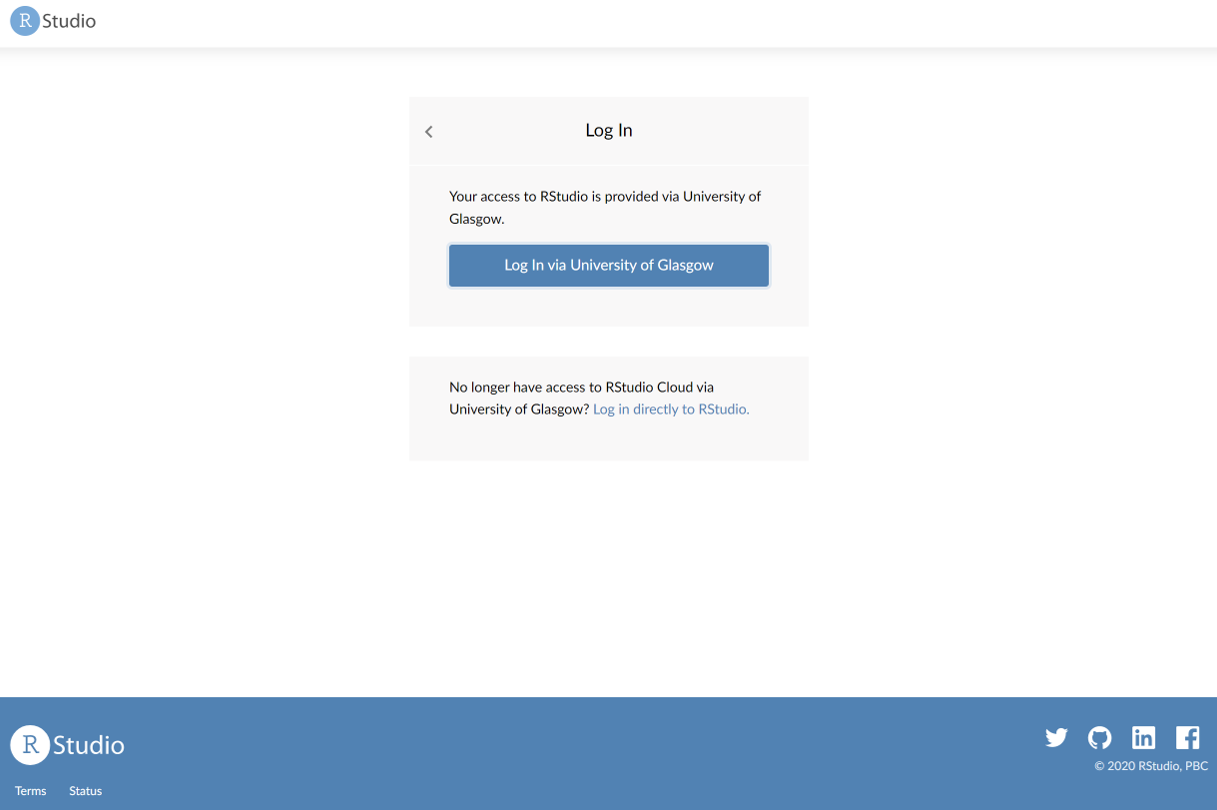
\includegraphics[width=1\linewidth]{./images/sso_login} \hfill{}

\caption{SSO Login}

\label{fig:unnamed-chunk-2}
\textbackslash end\{figure\}
4. Done! You will be taken you into your own Rstudio Cloud work space.

\textbf{Part 2} Join your lab group.

\begin{enumerate}
\def\labelenumi{\arabic{enumi}.}
\tightlist
\item
  You will receive a link from your tutor to join your lab group on RStudio Cloud (the link will be posted on Moodle too). N.b. you must use this specific link to join and access your lab group workspace, as each link is unique to your group. So only use your group's specific link. Copy and paste the link in your web browser. You should see the following window:
  \textbackslash begin\{figure\}
\end{enumerate}

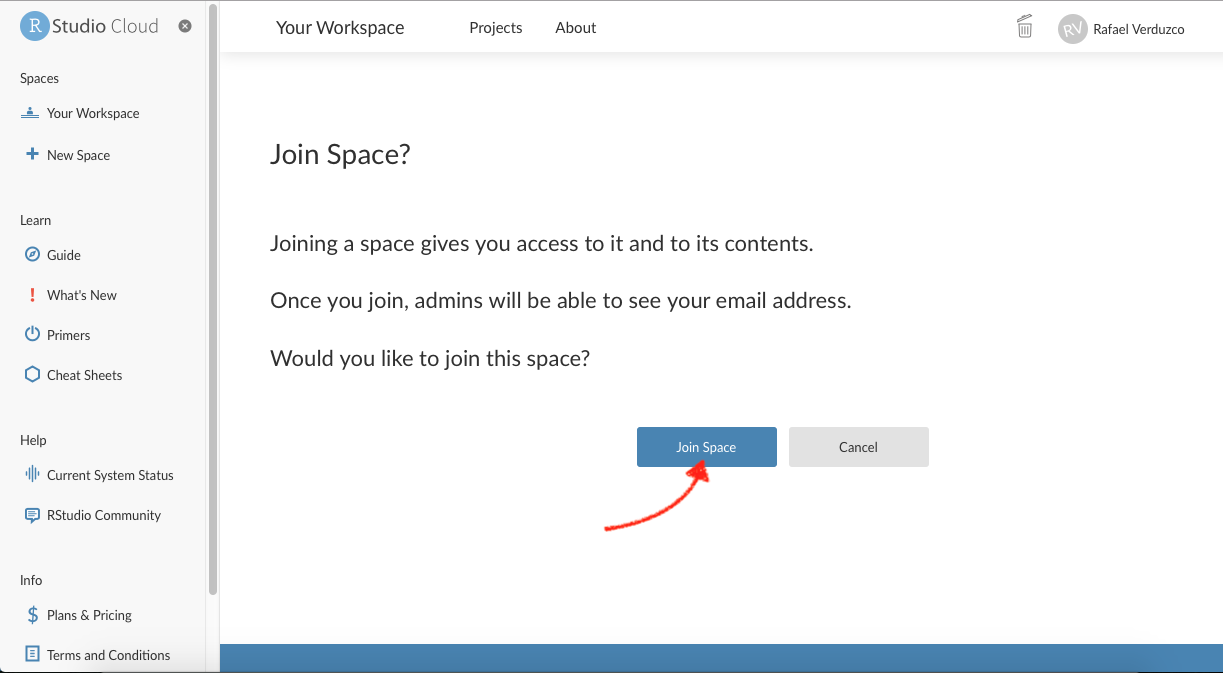
\includegraphics[width=1\linewidth]{./images/rstudio_cloud_joinspace} \hfill{}

\caption{Join Space.}

\label{fig:unnamed-chunk-3}
\textbackslash end\{figure\}
2. Join your lab by clicking on the `Join space' button shown above.
3. Open the shared space form the left-hand side pane called `Quants Lab Group..' and start the Lab 1 project by clicking on the `Start' button as shown below:

\begin{figure}

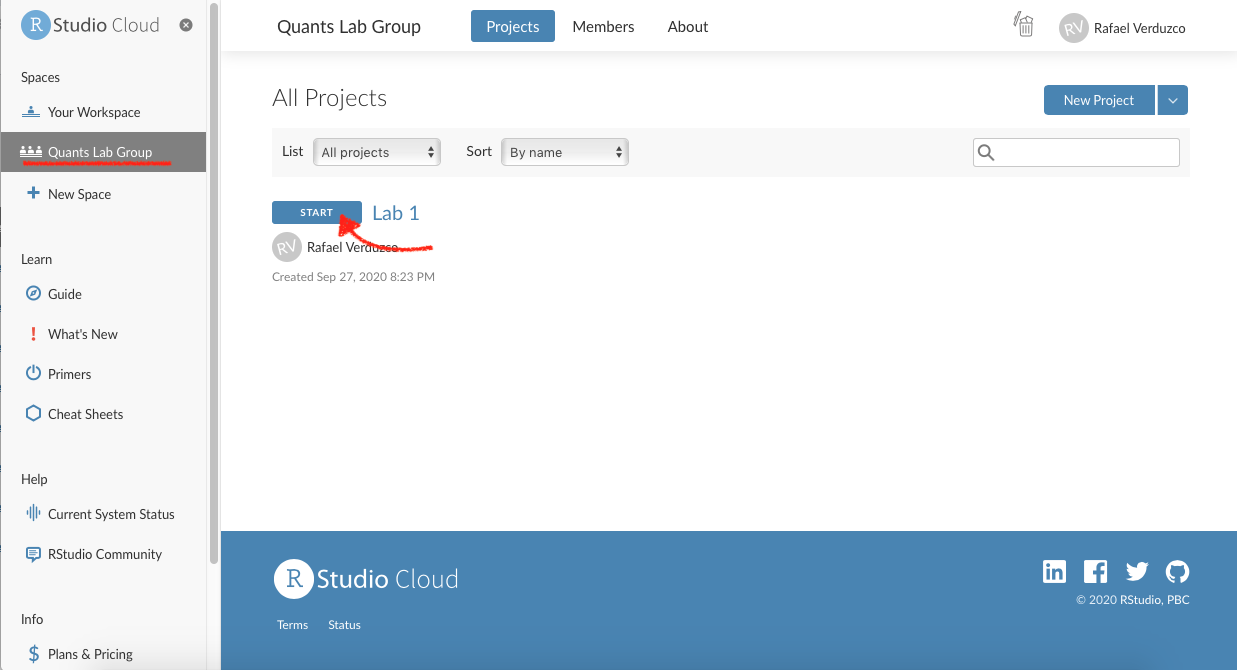
\includegraphics[width=1\linewidth]{./images/rstudio_cloud_startproject} \hfill{}

\caption{Start project.}\label{fig:unnamed-chunk-4}
\end{figure}

\hypertarget{rstudio-environment}{%
\subsection{RStudio environment}\label{rstudio-environment}}

\hypertarget{rstudio-screen}{%
\subsubsection{RStudio screen}\label{rstudio-screen}}

Once you have started `Lab 1' you will see the screen below.

\begin{figure}

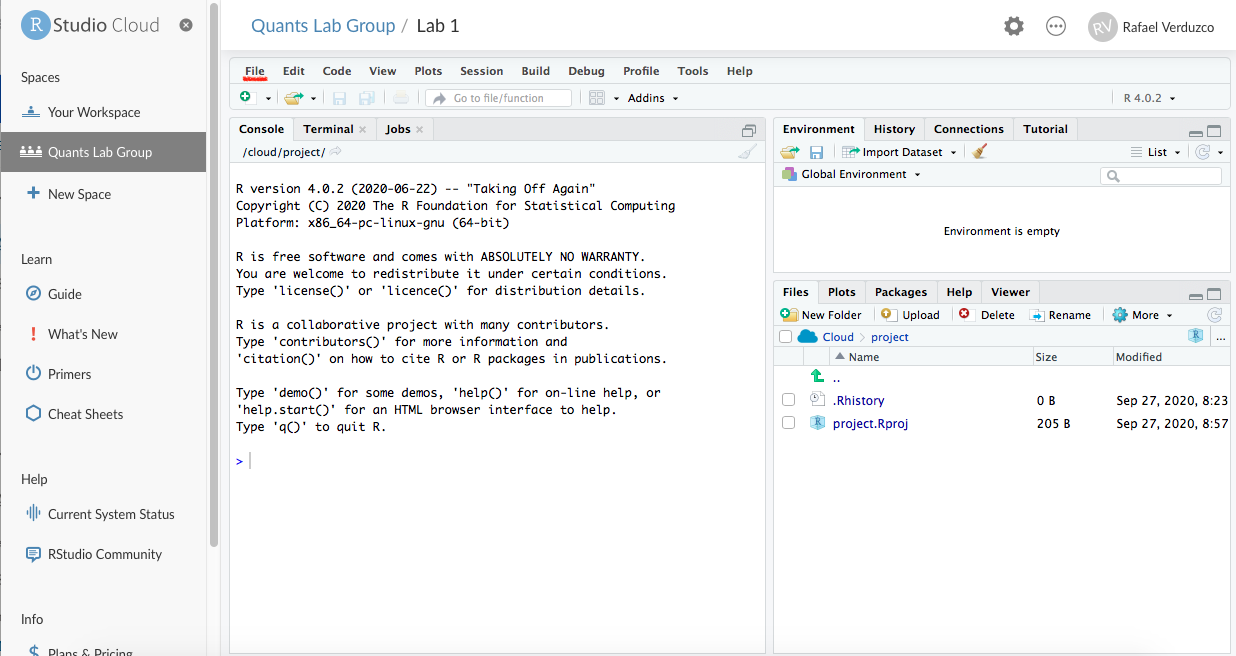
\includegraphics[width=1\linewidth]{./images/rstudio_cloud_lab1_empty} \hfill{}

\caption{Project name.}\label{fig:unnamed-chunk-5}
\end{figure}

Now, go to the ``File'' tab and create a R Script as follows \texttt{File\ \textgreater{}\ New\ file\ \textgreater{}\ R\ Script}

\begin{figure}

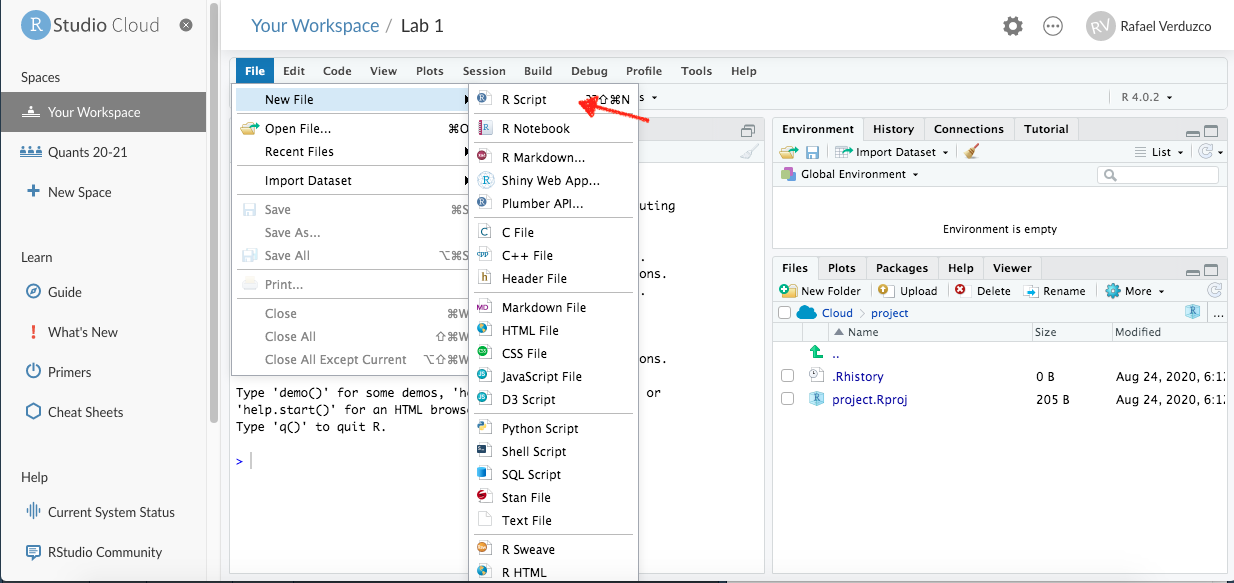
\includegraphics[width=1\linewidth]{./images/rstudio_cloud_new_script} \hfill{}

\caption{New R Script.}\label{fig:unnamed-chunk-6}
\end{figure}

Once you have created your first R Script, save it by clicking on File \textgreater{} Save as.. \textgreater{} \texttt{{[}write\ the\ name\ of\ your\ file{]}}.

After this, your RStudio screen will be split in four \textbf{important} windows or panes as shown below:

\begin{figure}

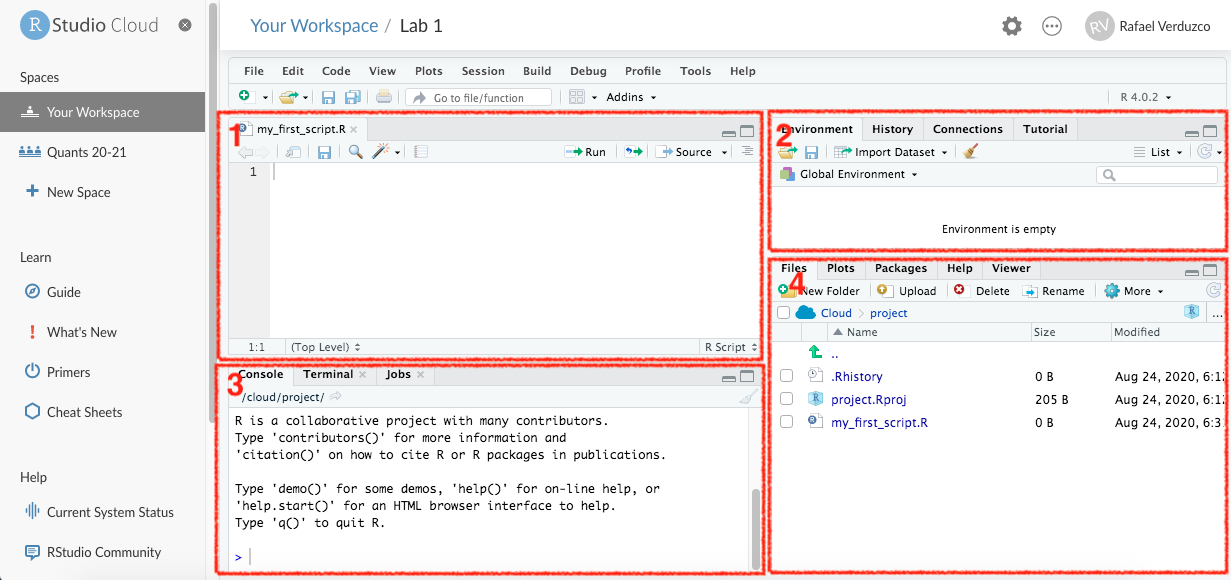
\includegraphics[width=1\linewidth]{./images/rstudio_cloud_panels} \hfill{}

\caption{R Studio panes.}\label{fig:unnamed-chunk-7}
\end{figure}

\begin{itemize}
\tightlist
\item
  In \textbf{Pane 1}, you have your newly created \texttt{R} script. This is the area where you will be working most of the time. From here, you will write functions. To run an \texttt{R} script line, you can click on the \texttt{Run} green arrow situated on the top of pane 1 or more commonly you can run a code line by typing \texttt{alt\ +\ enter}. The things you write in this section will be saved in your R script file.
  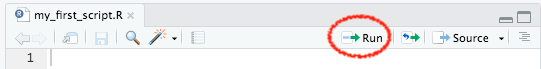
\includegraphics{./images/rstudio_cloud_run_button.png}
\item
  In \textbf{Pane 2}, you have the ``Global Environment'', this is one of the most useful tabs in this pane. It shows you the active `objects' that you have available/loaded in your current session (this will probably make more sense in the coming sections).
\item
  In \textbf{Pane 3}, you have the R Console, this is where you will see most of the results of the functions you run from your script (pane 1). You can also write and run functions from here, by typing the function and hitting enter. NOTE that what you do here will NOT be saved, this is usually used to quickly call functions that you do not want to save in your script.
  \textbackslash begin\{figure\}
\end{itemize}

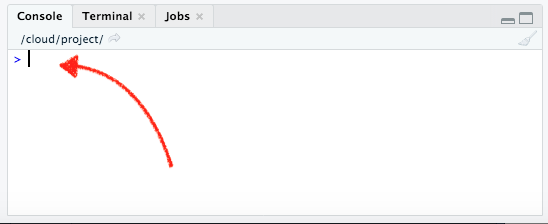
\includegraphics[width=1\linewidth]{./images/rstudio_cloud_console} \hfill{}

\caption{Console.}

\label{fig:unnamed-chunk-8}
\textbackslash end\{figure\}
* Finally, in \textbf{Pane 4} you have multiple useful tabs. In the \texttt{File} tab you can see the files and directories that you have in your R project. In the \texttt{Plot} tab you will see a preview of the static plots/charts you will be producing from your script. In \texttt{Packages}, you have a list of the extensions or plug-ins (called `packages' in R) that are installed in your working environment. The \texttt{Help} contains some resources that clarify or expand what each of the functions does. Again, probably this will make more sense once you get started. We will come back to this later. Finally, the \texttt{Viewer} displays interactive outputs.

\hypertarget{hands-on-r}{%
\section{Hands on R}\label{hands-on-r}}

Now you are ready! It is your turn to start exploring and getting familiar with R by completing the following activities.
5
\#\#\#\# R as calculator

Go to your \textbf{console} (pane 3, bottom-left pane), write some simple calculations and run them by typing `enter' after each of them, as shown below.

\begin{figure}

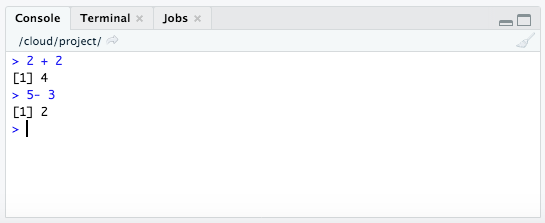
\includegraphics[width=1\linewidth]{./images/rstudio_cloud_r_as_calculator} \hfill{}

\caption{R Console as calculator.}\label{fig:unnamed-chunk-9}
\end{figure}

Try different operations such as \texttt{50\ /\ 20} or \texttt{3\ *\ 5}.

Fairly simple, right? And don't forget, it is entirely normal to copy/paste and tweak any existing codes. Unlike writing an essay or an exam, you don't actually need to know and write codes ``off the cuff'' or recite/memorise any syntax. You are only expected to know how to run the codes and tweak them as you go along, there is a huge amount of trial and error when you work in R. So don't worry if you feel like you are just making minor changes to the codes, that's how it's supposed to work, and the first few weeks is all about getting comfortable in using R, then the level of challenge will go up. Let's continue with the next activities!

\hypertarget{testing-logical-operators}{%
\subsubsection{Testing logical operators}\label{testing-logical-operators}}

Now, write and run the following lines in your \textbf{console} (pane 3) and take some time to observe the result in detail for each of them:

\begin{itemize}
\tightlist
\item
  \texttt{10\ ==\ 10}
\item
  \texttt{10\ !=\ 10}
\item
  \texttt{1\ ==\ 5}
\item
  \texttt{1\ \textgreater{}\ 5}
\item
  \texttt{\textquotesingle{}a\textquotesingle{}\ ==\ \textquotesingle{}a\textquotesingle{}}
\item
  \texttt{\textquotesingle{}a\textquotesingle{}\ ==\ \textquotesingle{}b\textquotesingle{}}
\end{itemize}

What do you see? \ldots{}

\ldots That's it! When you use the double equal sign \texttt{==} you are \emph{asking} R whether the value on the left hand-side of the operator is equal to the one on the right hand-side. Likewise, when you combine the exclamation mark \texttt{!} with other operator, you get the reversed result. In the past exercises you used \texttt{!=}, this was interpreted as ``is not equal to'', that is why \texttt{10\ !=\ 10} returns \texttt{FALSE}, but \texttt{10\ ==\ 10} returns \texttt{TRUE}.

\texttt{R} can process different classes of inputs. In this case we used letters and we \emph{asked} R whether `a' was equal to `a', and of course the result is \texttt{TRUE}. Note that when you want to input text (referred as \emph{character} values in R), you need quotation marks \texttt{\textquotesingle{}}. If you want to enter numeric values, you simply input the raw number. These are different `class' values.

Perhaps logical operators do not make much sense at this point, but you will find out later that they are useful to manipulate data. For example, these are essential to filter a data set based on specific \emph{rules} or patterns.

\hypertarget{assigning-values-to-objects}{%
\subsubsection{Assigning values to `objects'}\label{assigning-values-to-objects}}

In \texttt{R}, it is very common (and practical) to store values or data as `objects'. These are temporally stored in your current session. Let's try it!

Now, we will work in the \texttt{R} script file (\textbf{Pane 1}, top-left pane), write the following and run it by clicking the green arrow or using \texttt{alt\ +\ enter}:

\begin{Shaded}
\begin{Highlighting}[]
\NormalTok{a }\OtherTok{\textless{}{-}} \DecValTok{10}
\NormalTok{a }\SpecialCharTok{+} \DecValTok{5}
\end{Highlighting}
\end{Shaded}

What do you observe?\ldots{}

\ldots That's right! The operator \texttt{\textless{}-} assigned the numeric value \texttt{10} to the object \texttt{a} (on the left hand-side of the arrow). Later, you used the object (\texttt{a}) to compute a sum (i.e, \texttt{a\ +\ 5}).

Now, write and run the following in your \texttt{R} script (Pane 1)

\begin{Shaded}
\begin{Highlighting}[]
\NormalTok{c }\OtherTok{\textless{}{-}} \DecValTok{3}
\NormalTok{a  }\SpecialCharTok{*}\NormalTok{  c}
\end{Highlighting}
\end{Shaded}

As you can see, you stored the numeric value \texttt{3} in the variable \texttt{c}. Then, you called the previously created object \texttt{a} in a multiplication.

In the same way as you assigned these simple variables, you will store other types of objects later, e.g.~vectors, data frames or lists. This is useful because those objects will be ready in your session to do some computations.

There are a few things to note when assigning objects to variables. If you use a different value to the same variable, e.g.~by typing \texttt{a\ \textless{}-\ 5}, you will replace the old value with the new. So, instead of having \texttt{a} representing the value 10, you will have \texttt{5}. You can see the objects available in your session on the Global Environment (`Environment' tab in Pane 2) as shown below.

\begin{figure}

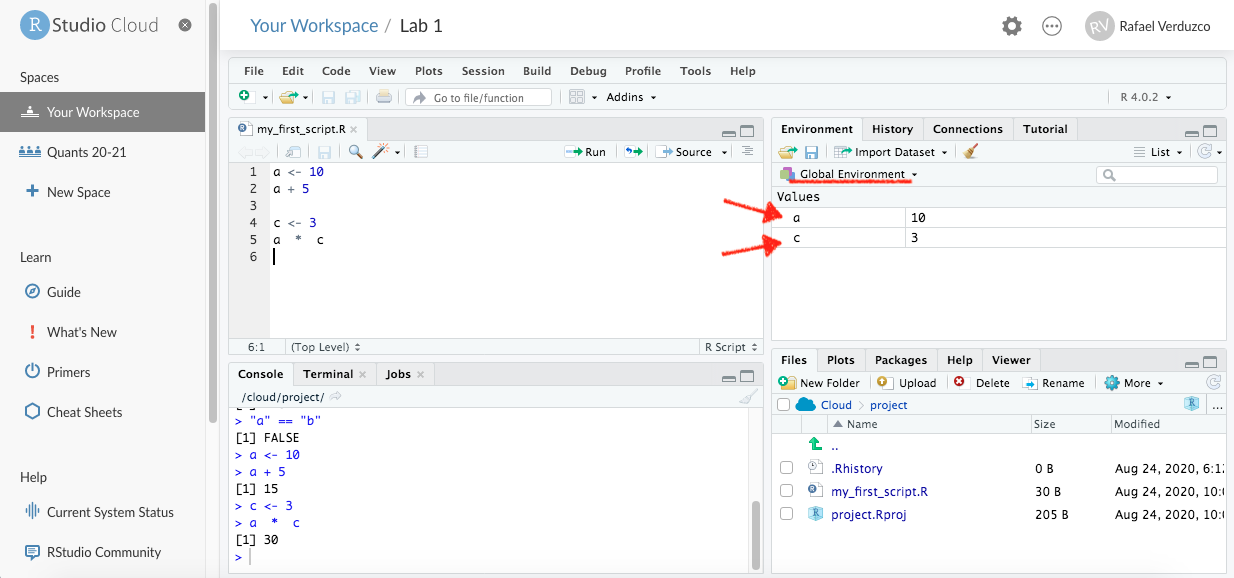
\includegraphics[width=1\linewidth]{./images/rstudio_cloud_environment} \hfill{}

\caption{'Environment' tab.}\label{fig:unnamed-chunk-12}
\end{figure}

This is a very good start, great job!

Note that the changes made in your script are saved automatically in RStudio Cloud. To verify this, have a look at the name of your script in the top-left of pane 1. If changes are due to be saved, the name will be written in red. If it is in red, save changes manually by clicking on the disk icon. After you have made sure your changes are saved, end your session simply by closing the RStudio Cloud tab in your browser.

\hypertarget{activity}{%
\section{Activity}\label{activity}}

Discuss the following questions with your neighbour or tutor:

\begin{enumerate}
\def\labelenumi{\arabic{enumi}.}
\tightlist
\item
  What are the main differences between working on a \texttt{R} script file (pane 1) and directly on the console (pane 3)?
\item
  Can you describe what happens when your run the following code? (tip: look at the environment tab in pane 2)
\end{enumerate}

\begin{Shaded}
\begin{Highlighting}[]
\NormalTok{object1 }\OtherTok{\textless{}{-}} \DecValTok{10}
\NormalTok{object1 }\OtherTok{\textless{}{-}} \DecValTok{30}
\end{Highlighting}
\end{Shaded}

\hypertarget{lab2}{%
\chapter{Data in R}\label{lab2}}

\hypertarget{welcome-back}{%
\section{Welcome back!}\label{welcome-back}}

In our previous lab, we set up an RStudio Cloud session and we got familiar with the RStudio environment and some of the purpose and contents of its panes. In this Lab we will learn about R packages, how to install them and load them. Also, we will use different types of data. You will have the chance to practice with additional \texttt{R} operators. Lastly, we will load a real-world data set and put in practice your new skills.

\hypertarget{learn-packages}{%
\section{R Packages}\label{learn-packages}}

As mentioned in our last lab, \texttt{R} \citep{R-base} is a collaborative project. This means that \texttt{R} users are developing, maintaining, and extending the functionalities constantly. When you set up \texttt{R} and RStudio for the first time, as we did it last week, it comes only with the `basic' functionalities by default. However, there are literally thousands of extensions that are developed by other users. In R, these non-default extensions are called \emph{\textbf{packages}}.

Most of the times, we use packages because they simplify our work in \texttt{R} or they allow us to extend the capabilites of base R.

\hypertarget{installing-packages}{%
\subsection{Installing packages}\label{installing-packages}}

Let's put hands-on to install and load some useful packages. We will start with \texttt{tidyverse} \citep{R-tidyverse}.\footnote{\url{https://www.tidyverse.org/}}

\hypertarget{activity-1}{%
\subsection{Activity:}\label{activity-1}}

\textbf{Part 1}. Access your lab group in R Studio Cloud

\begin{enumerate}
\def\labelenumi{\arabic{enumi}.}
\tightlist
\item
  Make sure you have a free, institutional-subscription \href{https://rstudio.cloud/}{RStudio Cloud} account (in case you have not created one yet, please follow the guidance provided in \protect\hyperlink{lab-intro}{Lab 1});
\item
  You will receive a link from your tutor to join your lab group in a shared space. Copy and paste it in your web browser (log in if necessary). If you already joined your lab group in RStudio Cloud, simply access the `Lab 2' project and omit steps 3 to 5. Otherwise, continue with steps 3, 4 and 5.
\item
  If you did not join your lab group yet, you should see the following window:
  \textbackslash begin\{figure\}
\end{enumerate}

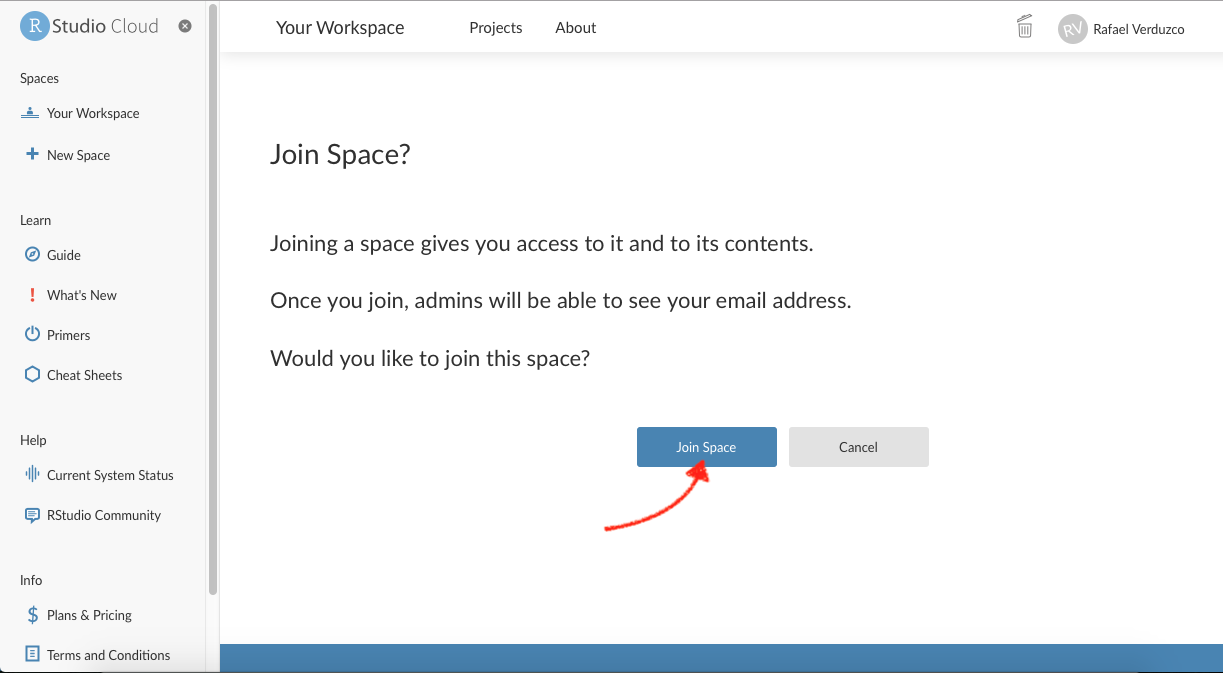
\includegraphics[width=1\linewidth]{./images/rstudio_cloud_joinspace} \hfill{}

\caption{Join Space}

\label{fig:unnamed-chunk-14}
\textbackslash end\{figure\}
4. Click on the `Join space' button shown above.
5. Open the shared space form the left-hand side pane called `Quants Lab Group..' and start the Lab 2 project by clicking on the `Start' button as shown below:

\begin{figure}

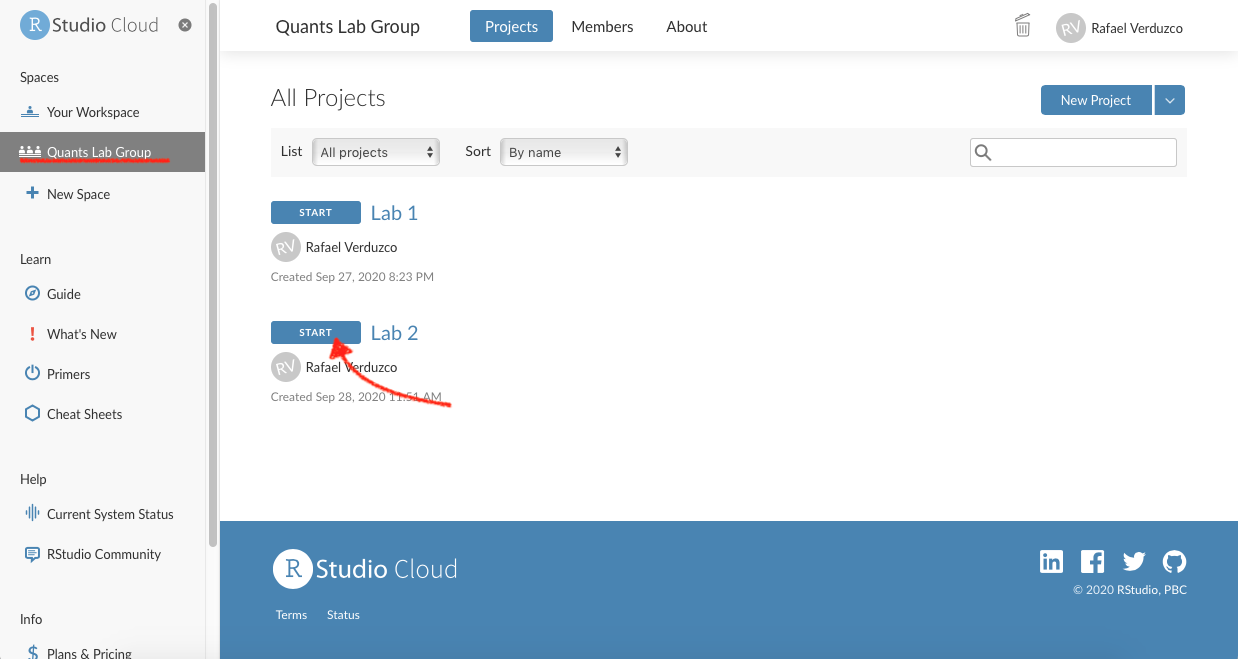
\includegraphics[width=1\linewidth]{./images/rstudio_cloud_startproject_lab2} \hfill{}

\caption{Start Lab 2.}\label{fig:unnamed-chunk-15}
\end{figure}

\textbf{Part 2}. Working on your script

\begin{enumerate}
\def\labelenumi{\arabic{enumi}.}
\tightlist
\item
  Once you have accessed the `Lab 2' project, write or copy the following line in your \textbf{script} (pane 1) and run it:
\end{enumerate}

\begin{Shaded}
\begin{Highlighting}[]
\FunctionTok{install.packages}\NormalTok{(}\StringTok{\textquotesingle{}tidyverse\textquotesingle{}}\NormalTok{)}
\end{Highlighting}
\end{Shaded}

\begin{enumerate}
\def\labelenumi{\arabic{enumi}.}
\setcounter{enumi}{1}
\tightlist
\item
  Wait until you get the message `The downloaded source packages are in\ldots{}'. The installing process can take up to a couple of minutes to finish.
\item
  Once the package is installed, you need to load it using the \texttt{library()} function. Please, copy and paste the following line, and run it:
\end{enumerate}

\begin{Shaded}
\begin{Highlighting}[]
\FunctionTok{library}\NormalTok{(tidyverse)}
\end{Highlighting}
\end{Shaded}

And that's it, \texttt{tidyverse} is ready to be used in your current session!

There are couple of things you should know. First, the packages need to be installed only per project in RStudio Cloud (and only once if you are working in RStudio Desktop version). However, packages must be loaded using the \texttt{library()} function every time you restart an R session.

Another thing to notice is that when you install a package you need to use quotation marks, whereas in \texttt{library()} you only need to write the plain package name within brackets. Usually, you will load the packages at the beginning of your script.

\hypertarget{types-of-variables}{%
\section{Types of variables}\label{types-of-variables}}

\texttt{R} can handle many classes of data. It is crucial that you can distinguish the main ones. Broadly speaking there are two types of variables,

\begin{enumerate}
\def\labelenumi{\arabic{enumi}.}
\tightlist
\item
  \textbf{categorical} and;
\item
  \textbf{numeric} (formally know as interval or ratio).
\end{enumerate}

Categorical variables are distinctive because they are limited in the number of categories it can take, e.g., country, name, political party, or gender. Ordinal data is a \emph{sub-type} of the categorical, and it is used when the categories can be ranked and their order is meaningful, e.g., education level or level of satisfaction. Numeric values can be continuous (these are usually measured and can take infinite values, e.g.~speed or time).\footnote{For more details, please refer to the DataCamp module \href{https://learn.datacamp.com/courses/introduction-to-data-in-r}{Introduction to Data in R}.}

In \texttt{R}, the basic types of data are known as `atomic vectors' and there are 6 of them (logical, integer, double, character, complex and raw). In the social sciences, we often use the following: \texttt{numeric}, \texttt{factor} and \texttt{character}. Numeric vectors are used to represent continuous numerical data.\footnote{Notice that \texttt{numeric} vectors can be represented as \texttt{integer}or \texttt{double} in \texttt{R}, their difference is of little relevance for now.} On the other hand, factor vectors are used to represent categorical and ordinal data.

In R, there are couple of functions that will help us to identify the type of data. First, we have \texttt{glimpse()}. This prints some of the main characteristics of a data set, namely its overall dimension, name of each variable (column), the first values for each variable, and the type of the variable. Second we have the function \texttt{class()}, that will help us to determine the overall class(type) of on \texttt{R} object.

\hypertarget{activity-2}{%
\subsection{Activity:}\label{activity-2}}

We are now going to use some datasets that are pre-loaded in the \texttt{R} session by default. Please go to your `Lab\_2' project in RStudio Cloud and do the following:

\begin{enumerate}
\def\labelenumi{\arabic{enumi}.}
\tightlist
\item
  We will start with a classic dataset example in R called \texttt{iris}. This contains measurements of various flowers species (for more info type \texttt{?iris} in your console). Please go to your \textbf{console} and type the line below.
\end{enumerate}

\begin{Shaded}
\begin{Highlighting}[]
\FunctionTok{glimpse}\NormalTok{(iris)}
\end{Highlighting}
\end{Shaded}

\begin{enumerate}
\def\labelenumi{\arabic{enumi}.}
\setcounter{enumi}{1}
\tightlist
\item
  What do you observe from the output?\ldots{} First, it tells you the number of rows and the columns on the top. Later, it lists the name of each variable. Additionally, it tells you the type of the variable between these symbols \texttt{\textless{}\ \textgreater{}}. The first five variables in this dataset are of type \texttt{\textless{}dbl\textgreater{}} which is a type of numeric variable. The last, \texttt{Species}, is a factor \texttt{\textless{}fct\textgreater{}}. In sum, there is information of the species and four types of continuous measures associated to each flower in this dataset.
\item
  Now you know that each flower belongs to a species, but what are the specific categories in this data set? To find out, type the following in your console.
\end{enumerate}

\begin{Shaded}
\begin{Highlighting}[]
\FunctionTok{levels}\NormalTok{(iris}\SpecialCharTok{$}\NormalTok{Species)}
\end{Highlighting}
\end{Shaded}

\begin{enumerate}
\def\labelenumi{\arabic{enumi}.}
\setcounter{enumi}{3}
\tightlist
\item
  As you can see, there are three categories, which are three types of flower species. In \texttt{R} the categories in factor vectors are are called \emph{levels}.
\end{enumerate}

Note the syntax above. Inside the function, we used the name of the dataset followed by the dollar sign (\$) which is is needed to access the specific column/variable \texttt{Species}.

Now, let's get serious and explore Star Wars. Yes, the famous film series!

The \texttt{starwars} data set from the \texttt{dplyr} package contains information about the characters, including height, hair colour, and sex (to get more information type \texttt{?starwars} in your console). At this time we will use a reduced version of the full data set. Please complete the following activities from your \texttt{R} script (pane 1).

\begin{enumerate}
\def\labelenumi{\arabic{enumi}.}
\tightlist
\item
  First, we will run the next couple of lines to reduce the data set, and then we will glimpse the Star Wars characters:
\end{enumerate}

\begin{Shaded}
\begin{Highlighting}[]
\NormalTok{starwars2 }\OtherTok{\textless{}{-}}\NormalTok{ starwars[ ,}\DecValTok{1}\SpecialCharTok{:}\DecValTok{11}\NormalTok{]}
\FunctionTok{glimpse}\NormalTok{(starwars2)}
\end{Highlighting}
\end{Shaded}

\begin{enumerate}
\def\labelenumi{\arabic{enumi}.}
\setcounter{enumi}{1}
\tightlist
\item
  What do you observe this time? \ldots{} It seems that the data type is not consistent with their content. For example, the variables \texttt{species}, \texttt{gender}, and \texttt{hair\_color} are of type \texttt{\textless{}chr\textgreater{}} (that is \texttt{character}), when according to what we just learnt they should be a factor. To transform them, we will use the function ´factor()´. This process is known as coercing a variable, that is when you change from one type to another.
\item
  Let's coerce the species variable from character to factor and assign the result to the same column in the dataset.
\end{enumerate}

\begin{Shaded}
\begin{Highlighting}[]
\NormalTok{starwars2}\SpecialCharTok{$}\NormalTok{species }\OtherTok{\textless{}{-}} \FunctionTok{factor}\NormalTok{(starwars2}\SpecialCharTok{$}\NormalTok{species)}
\end{Highlighting}
\end{Shaded}

\begin{enumerate}
\def\labelenumi{\arabic{enumi}.}
\setcounter{enumi}{6}
\tightlist
\item
  Let's check if the type of variable really changed by glimpsing the data and checking the levels of \texttt{species}.
\end{enumerate}

\begin{Shaded}
\begin{Highlighting}[]
\FunctionTok{glimpse}\NormalTok{(starwars2)}
\FunctionTok{levels}\NormalTok{(starwars2}\SpecialCharTok{$}\NormalTok{species)}
\end{Highlighting}
\end{Shaded}

The glimpse result now is telling us that \texttt{species} is a \texttt{\textless{}fct\textgreater{}}, as expected. Furthermore, the \texttt{levels()} function reveals that there are 37 types of species, including Human, Ewok, Droid, and more.

Hopefully, these examples will help you to identify the the main vector types and more importantly to coerce them in an appropriate type. Be aware that many data sets represent categories with numeric values, for example, using `0' for males and `1' for females. Usually, large data sets are accompanied by extra information in a \emph{code book} or \emph{documentation} file, which specifies the values of the numeric code and their respective meaning. It's important to read the code book/documentation of every dataset as the conventions and meanings can vary.

\hypertarget{more-operators-and-some-essential-symbols}{%
\section{More operators and some essential symbols}\label{more-operators-and-some-essential-symbols}}

A useful operator is the pipe \texttt{\%\textgreater{}\%}. This is part of the \texttt{tidyverse} package. So, it is ready for you to use. This operator passes the result of one operation to the next. Check the results of the following operations in your \textbf{console}:

\begin{Shaded}
\begin{Highlighting}[]
\DecValTok{1} \SpecialCharTok{\%\textgreater{}\%} \SpecialCharTok{+} \DecValTok{1}
\DecValTok{1} \SpecialCharTok{\%\textgreater{}\%} \SpecialCharTok{+} \DecValTok{1} \SpecialCharTok{\%\textgreater{}\%} \SpecialCharTok{+} \DecValTok{5}
\end{Highlighting}
\end{Shaded}

Observe what happened\ldots The result from the first line was 2. This is because this line can be read as: `take 1, THEN sum 1'. Therefore, the result is 2.

Similarly, the second line follows this process: `take 1, THEN sum 1, take the result of this (which is '2') and THEN sum 5'. Therefore, the result is 7. This can sound a bit abstract at this point, but we will practice with some data in the next section.

\hypertarget{black-lives-matter}{%
\section{Black lives matter!}\label{black-lives-matter}}

In this section we will work with data originally collected by The Guardian in 2015, for more information click \href{https://www.theguardian.com/us-news/ng-interactive/2015/jun/01/about-the-counted}{here}. The data set we will use today is an extended version which was openly shared in GitHub by the American news website \href{https://fivethirtyeight.com/}{FiveThirtyEight}. This data set contains information about the people that were killed by police or other law enforcement bodies in the US, such as age, gender, race/ethnicity, etc. Additionally, it includes information about the city or region where the event happened. For more information click \href{https://github.com/fivethirtyeight/data/tree/master/police-killings}{here}.

\hypertarget{downloading-and-reading-the-data}{%
\subsection{Downloading and reading the data}\label{downloading-and-reading-the-data}}

For the following excercices, please make sure that your are working in your \texttt{R} script.

First, we will create a new folder in our project directory to store the data. To do it from \texttt{R}, run this line in your script (Don't worry if you get a warning. This appears because you already have a folder with this name):

\begin{Shaded}
\begin{Highlighting}[]
\FunctionTok{dir.create}\NormalTok{(}\StringTok{"data"}\NormalTok{)}
\end{Highlighting}
\end{Shaded}

Note that in the `Files' tab of Pane 4, there is a new folder called \texttt{data}.

Now, download the data from the GitHub repository using the function \texttt{download.file()}. This function takes two arguments separated by a comma: (1) the URL and (2) the destination (including the directory, file name, and file extension), as shown below. Also, since the file we downloaded is wrapped in a \texttt{.zip} file, we will need to unzip it using \texttt{unzip()}. Copy, paste in your script, the following lines:

\begin{Shaded}
\begin{Highlighting}[]
\FunctionTok{download.file}\NormalTok{(}\StringTok{"https://projects.fivethirtyeight.com/data{-}webpage{-}data/datasets/police{-}killings.zip"}\NormalTok{,}
              \StringTok{"data/police{-}killings.zip"}\NormalTok{)}
\FunctionTok{unzip}\NormalTok{(}\StringTok{"data/police{-}killings.zip"}\NormalTok{, }\AttributeTok{exdir =} \StringTok{"data"}\NormalTok{)}
\end{Highlighting}
\end{Shaded}

After following the previous steps, we are ready to read the data. As you can see in the `File' tab, the data comes as a \texttt{.csv} file. Thus, we can use the \texttt{read\_csv()} function included in the \texttt{tidyverse} package (make sure you the package is loaded in your session as explained in a \protect\hyperlink{installing-packages}{previous section}). We will assign the data in an object called \texttt{police}.

\begin{Shaded}
\begin{Highlighting}[]
\NormalTok{police }\OtherTok{\textless{}{-}} \FunctionTok{read\_csv}\NormalTok{(}\StringTok{"data/police{-}killings/police\_killings.csv"}\NormalTok{)}
\end{Highlighting}
\end{Shaded}

\hypertarget{examining-the-data}{%
\subsection{Examining the data}\label{examining-the-data}}

If you look at your `Environment' tab in pane 2, you will see there is a new object called \texttt{police}, which has 467 observations and 34 variables (or columns). To start exploring the contents, we will glimpse the \texttt{police} data as following:

\begin{Shaded}
\begin{Highlighting}[]
\FunctionTok{glimpse}\NormalTok{(police)}
\end{Highlighting}
\end{Shaded}

As you can see, there are several variables included in the dataset, such as age, gender, law enforcement agency (\texttt{lawenforcementagency}), or whether the victim was armed (\texttt{armed}). You will see some of these variables are not in the appropriate type. For instance, some are categorical and should be type \texttt{\textless{}fct\textgreater{}} instead of \texttt{\textless{}chr\textgreater{}}.

\hypertarget{data-wrangling}{%
\subsection{Data wrangling}\label{data-wrangling}}

Before coercing these variables, we will create a smaller subset selecting only the variables that we are interested in. To do so, we can use the \texttt{select()} function. The \texttt{select} function takes the name of the data first and then the name of the variables we want to keep (no quotation marks needed). We will select a few variables and assign the result to a new object called \texttt{police\_2}.

\begin{Shaded}
\begin{Highlighting}[]
\NormalTok{police\_2 }\OtherTok{\textless{}{-}} \FunctionTok{select}\NormalTok{(police, age, gender, raceethnicity, lawenforcementagency, armed)}
\end{Highlighting}
\end{Shaded}

If you look again to the `Environment' tab, there is a second data set with the same number of observations but only 5 variables. You can glimpse this object to have a better idea of its contents.

\begin{Shaded}
\begin{Highlighting}[]
\FunctionTok{glimpse}\NormalTok{(police\_2)}
\end{Highlighting}
\end{Shaded}

Having a closer look at the reduced version, we can see that in fact all the variables are of type \texttt{\textless{}chr\textgreater{}}, including \texttt{age}.

Let's coerce the variables in to their correct type. We will start with age, from character to numeric:

\begin{Shaded}
\begin{Highlighting}[]
\NormalTok{police\_2 }\OtherTok{\textless{}{-}}\NormalTok{ police\_2 }\SpecialCharTok{\%\textgreater{}\%} \FunctionTok{mutate}\NormalTok{(}\AttributeTok{age =} \FunctionTok{as.numeric}\NormalTok{(age))}
\end{Highlighting}
\end{Shaded}

Age is not known for some cases. Thus, it is recorded as `Unknown' in the dataset. Since this is not recognized as a numeric value in the coercion process, \texttt{R} automatically sets it as a missing value, \texttt{NA}. This is why it will give you a warning message.

We can continue coercing \texttt{raceethnicity} and \texttt{gender} from character to a factor:

\begin{Shaded}
\begin{Highlighting}[]
\NormalTok{police\_2 }\OtherTok{\textless{}{-}}\NormalTok{ police\_2 }\SpecialCharTok{\%\textgreater{}\%} \FunctionTok{mutate}\NormalTok{(}\AttributeTok{raceethnicity =} \FunctionTok{factor}\NormalTok{(raceethnicity))}
\NormalTok{police\_2 }\OtherTok{\textless{}{-}}\NormalTok{ police\_2 }\SpecialCharTok{\%\textgreater{}\%} \FunctionTok{mutate}\NormalTok{(}\AttributeTok{gender =} \FunctionTok{factor}\NormalTok{(gender))}
\end{Highlighting}
\end{Shaded}

Let's run a summary of your data. This shows the number of observations in each category or a summary of a numeric variable:

\begin{Shaded}
\begin{Highlighting}[]
\FunctionTok{summary}\NormalTok{(police\_2)}
\end{Highlighting}
\end{Shaded}

There are some interesting figures coming out from the summary. For instance, in age you can see that the youngest is\ldots{} 16 years old(?!), and the oldest 87 years old. Also, the vast majority are male individuals (445 vs 22). In relation to race/ethnicity, roughly half of them is `White', whereas `Black' individuals represent an important share. One may question about the proportion of people killed in terms of race/ethnicity compared to the composition of the total population (considering Black is a minority group in the US).

Let's suppose that we only want observations in which race/ethnicity is not unknown. To `remove' \emph{undesired} observation we can use the \texttt{filter()} function. We will assign the result of \texttt{filter} in a variable called \texttt{police\_2}.

\begin{Shaded}
\begin{Highlighting}[]
\NormalTok{police\_2 }\OtherTok{\textless{}{-}}\NormalTok{ police\_2 }\SpecialCharTok{\%\textgreater{}\%} \FunctionTok{filter}\NormalTok{(raceethnicity }\SpecialCharTok{!=} \StringTok{\textquotesingle{}Unknown\textquotesingle{}}\NormalTok{)}
\end{Highlighting}
\end{Shaded}

So, what just happened in the code above? First, the pipe operator, \texttt{\%\textgreater{}\%}: What we are doing verbally is \emph{take the object \texttt{police\_2}, THEN filter raceethnicity based on a condition}. Later, what is happening inside \texttt{filter}? Lets have a look at what \texttt{R} does in the background for us (Artwork by @alison\_horst):

\begin{figure}

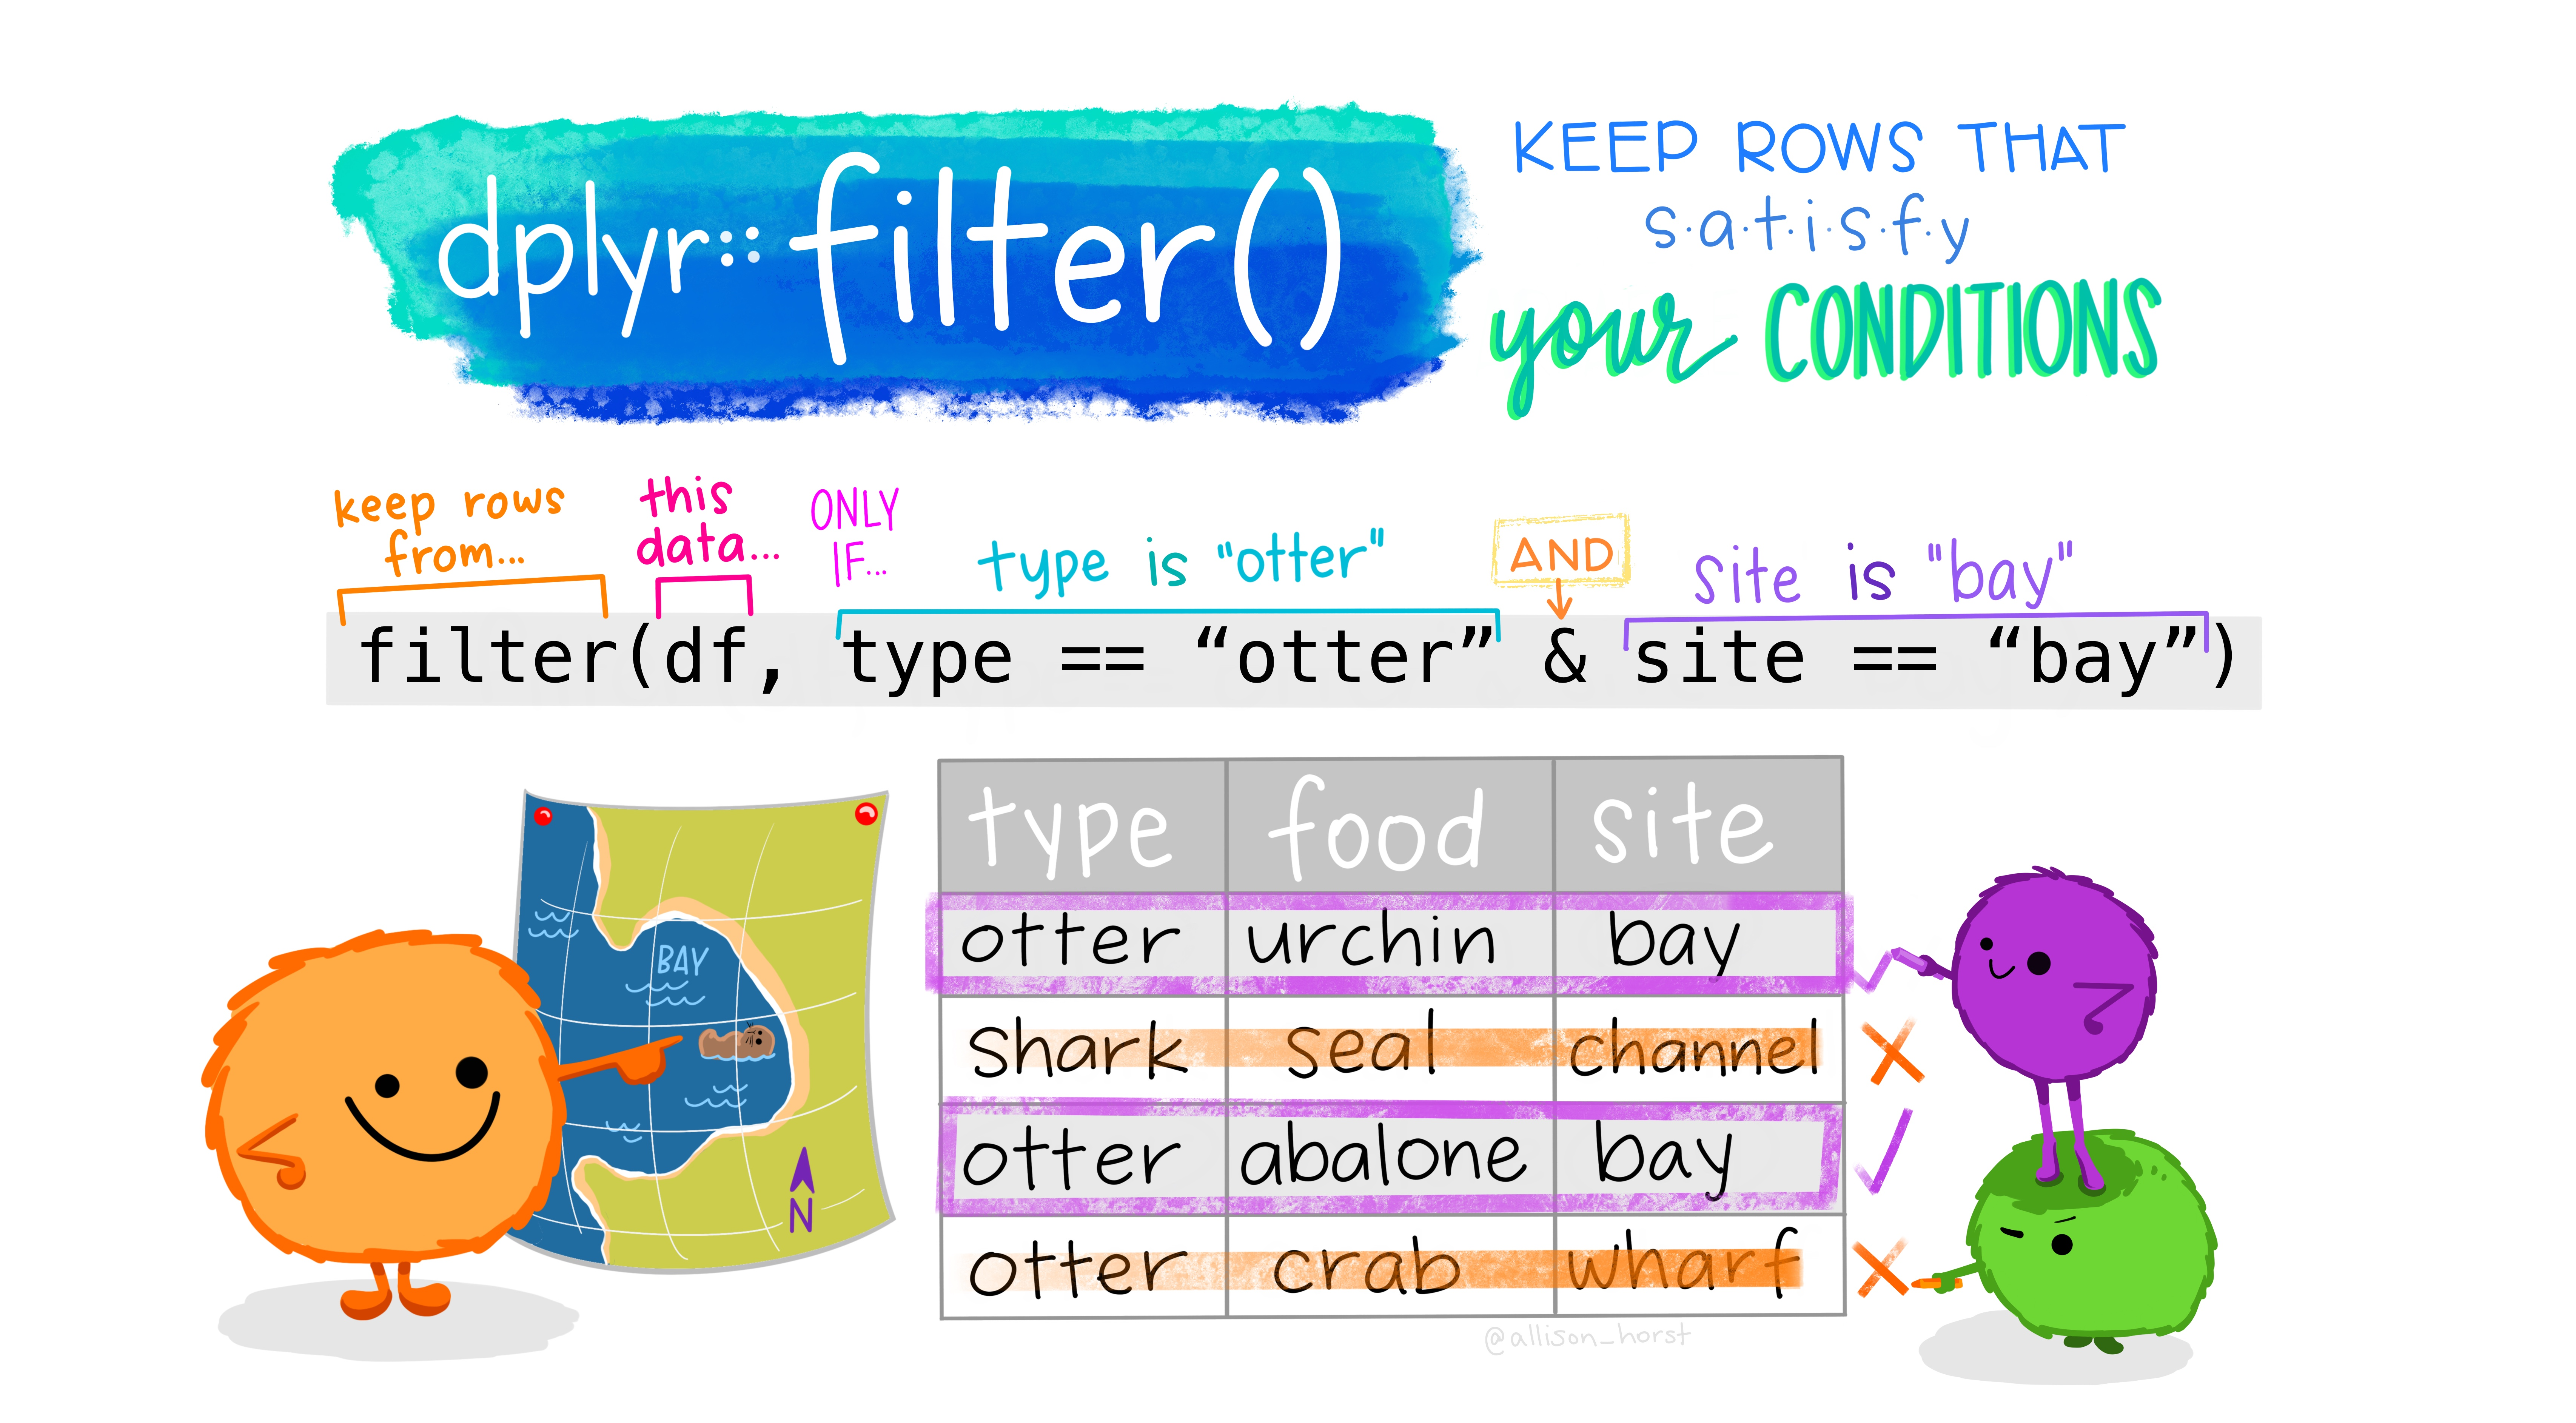
\includegraphics[width=1\linewidth]{./images/lab_2_filter} \hfill{}

\caption{Filter. Source: Artwork by @Horst.}\label{fig:unnamed-chunk-34}
\end{figure}

In the example above, we are keeping the observations in \texttt{raceethnicity} that are NOT EQUAL to `Unknown'. Finally, when we assigned the result to an object named as the same as our previous object, we replaced the \emph{old} dataset with the filtered version.

\hypertarget{activity-3}{%
\section{Activity}\label{activity-3}}

Discuss the following questions with your neighbour or tutor:

\begin{enumerate}
\def\labelenumi{\arabic{enumi}.}
\tightlist
\item
  What is the main purpose of the functions \texttt{select()} and \texttt{filter}?
\item
  What does \emph{coerce} mean in the context of \texttt{R}? and Why do we need to coerce some variables?
\item
  What is the \texttt{mutate()} function useful for?
\end{enumerate}

Using the police\_2 dataset:

\begin{enumerate}
\def\labelenumi{\arabic{enumi}.}
\tightlist
\item
  Filter how many observations are `White' in \texttt{raceethnicity}? How may rows/observations are left?
\item
  How many `Latino/Hispanic' are there in the dataset?
\item
  Using the example of Figure 2.3, could you filter how many were killed that were (a) `Black' and (b) killed by firearm (`firearm')?
\item
  What about `White' and `firearm'?
\end{enumerate}

This is the end of Lab 2. Again, the changes in your script should be saved automatically in R Studio Cloud. However, make sure this is the case as you were taught in Lab 1. After this, you can close the tab in your web browser. Hope you had fun!

\hypertarget{data-wrangling-1}{%
\chapter{Data wrangling}\label{data-wrangling-1}}

Welcome to Lab 3!

In our previous session we learned about \texttt{R} packages, including how to install and load them. We talked about the main types of data used in social science research and how to represent them in \texttt{R}. Also, we played around with some datasets using some key functions, such as: \texttt{filter()}, \texttt{select()}, and \texttt{mutate()}. In this session we will learn how to import data in \texttt{R}, clean and format the data using a real-world dataset. These is a common and important phase in quantitative research.

\hypertarget{importing-and-data-wrangling}{%
\section{Importing and data wrangling}\label{importing-and-data-wrangling}}

Today, we will be working with data generated by the \href{https://www.ark.ac.uk/ARK/}{Access Research Knowledge (ARK)} hub. ARK conducts a series of surveys about society and life in Northern Ireland. For this lab, we will be working with the results of the \href{https://www.ark.ac.uk/nilt/}{Northern Ireland Life and Times Survey (NILT)} in the year 2012. In particular, we will be using a teaching dataset that focuses on community relations and political attitudes. This includes background information of the participants and their household. Please take 5-10 minutes to read the documentation of this dataset (\href{https://www.ark.ac.uk/teaching/NILT2012TeachingResources.pdf}{click here to access the documentation}). p.s. You will have to regularly consult this document to understand and use the data in NILT. So, I recommend you to save the PDF file in your local drive if you can. This NILT teaching dataset is also what you will be using for the research report assignment in this course (smart, isn't it?) - so it's worth investing the time to learn how to work with this data through the next few labs, as part of the preparation and practice for your assignemnt.

\hypertarget{downloading-and-reading-the-data-1}{%
\subsection{Downloading and reading the data}\label{downloading-and-reading-the-data-1}}

We will continue using R Studio Cloud, as we did in our previous labs. Please follow the next steps:

\begin{enumerate}
\def\labelenumi{\arabic{enumi}.}
\tightlist
\item
  Go to your `Quants lab group' in \href{https://rstudio.cloud/}{RStudio Cloud} (if you have not joined a shared space, follow the instructions in \protect\hyperlink{learn-packages}{Section 2.2} of \protect\hyperlink{lab2}{Lab 2}).
\item
  Start the project called `NILT' located in your lab group.
\item
  Once you have initialized the project, generate a new \texttt{R} scrip file, and save it as `Exploratory analysis'.
\item
  Load the \texttt{tidyverse} and \texttt{haven} packages. This last package is useful to import data from SPSS (the \texttt{tidyverse} package was pre-installed in your session). You can copy, paste, and run the following functions from your script:
\end{enumerate}

\begin{Shaded}
\begin{Highlighting}[]
\FunctionTok{library}\NormalTok{(tidyverse)}
\FunctionTok{library}\NormalTok{(haven)}
\end{Highlighting}
\end{Shaded}

Next, we will create a folder to store the data. Then, download and read the NILT data set, following the next steps:

\begin{enumerate}
\def\labelenumi{\arabic{enumi}.}
\tightlist
\item
  From your script, create a new folder called `data':
\end{enumerate}

\begin{Shaded}
\begin{Highlighting}[]
\FunctionTok{dir.create}\NormalTok{(}\StringTok{\textquotesingle{}data\textquotesingle{}}\NormalTok{)}
\end{Highlighting}
\end{Shaded}

\begin{enumerate}
\def\labelenumi{\arabic{enumi}.}
\setcounter{enumi}{1}
\tightlist
\item
  Download the data using the \texttt{download.file()} function. Remember that you have to specify the URL first, and the destination of the file second (including the folder).
\end{enumerate}

\begin{Shaded}
\begin{Highlighting}[]
\FunctionTok{download.file}\NormalTok{(}\StringTok{\textquotesingle{}https://www.ark.ac.uk/teaching/NILT2012GR.sav\textquotesingle{}}\NormalTok{, }
              \StringTok{\textquotesingle{}data/nilt2012.sav\textquotesingle{}}\NormalTok{)}
\end{Highlighting}
\end{Shaded}

\begin{enumerate}
\def\labelenumi{\arabic{enumi}.}
\setcounter{enumi}{2}
\tightlist
\item
  Take a look to the `Files' tab in pane 3, you will see a folder called `data', click on it, and you will see the \texttt{nilt2012.sav} file.
  \textbackslash begin\{figure\}
\end{enumerate}

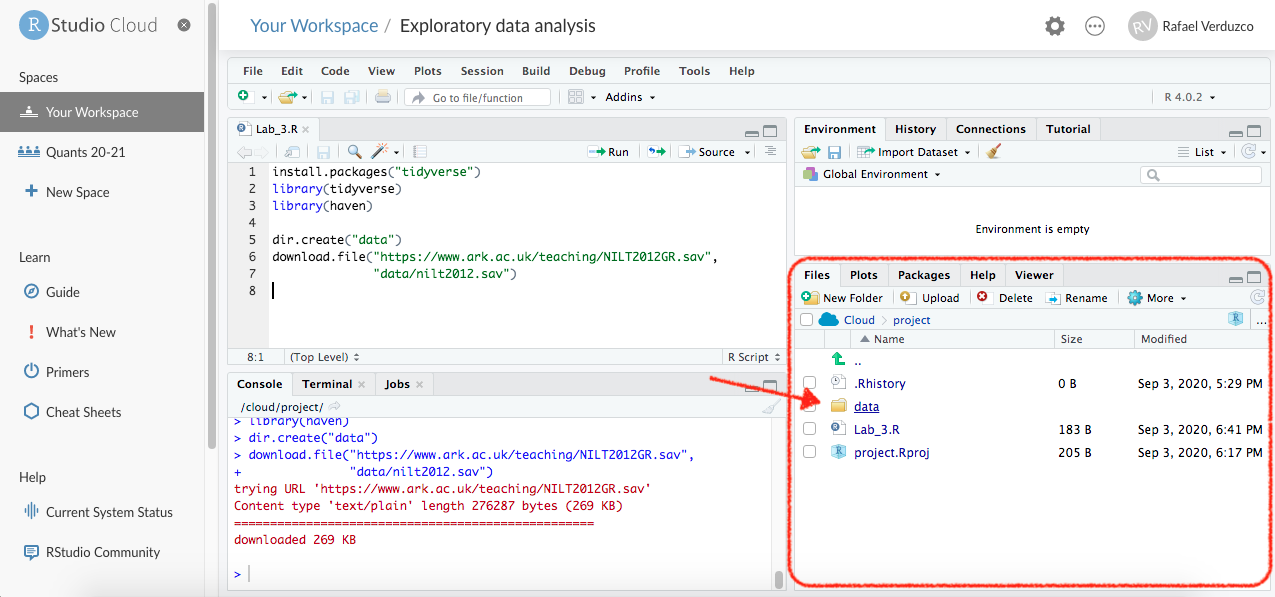
\includegraphics[width=1\linewidth]{./images/rstudio_cloud_files} \hfill{}

\caption{Cloud files.}

\label{fig:unnamed-chunk-38}
\textbackslash end\{figure\}
4. To read this type of file use the \texttt{read\_sav()} function. Read the \texttt{.sav} file and assign it to an object called \texttt{nilt}.

\begin{Shaded}
\begin{Highlighting}[]
\NormalTok{nilt }\OtherTok{\textless{}{-}} \FunctionTok{read\_sav}\NormalTok{(}\StringTok{"data/nilt2012.sav"}\NormalTok{)}
\end{Highlighting}
\end{Shaded}

And that's it! You should see a new data object in your `Environment' tab (Pane 2) ready to be used. You can also see that this contains 1204 observations (rows) and 133 variables (columns). Lets glimpse our newly imported data and see the type of variables included.

\begin{Shaded}
\begin{Highlighting}[]
\FunctionTok{glimpse}\NormalTok{(nilt)}
\end{Highlighting}
\end{Shaded}

\hypertarget{data-wrangling-2}{%
\section{Data wrangling}\label{data-wrangling-2}}

As you can see from the result of glimpse, the class for practically all the variables is \texttt{\textless{}dbl+lbl\textgreater{}}. What does this mean? This happened because usually datasets use numbers to represent each of the categories/levels in categorical variables. These numbers are \emph{labelled} with their respective meaning. This is why we have a combination of value types (\texttt{\textless{}dbl+lbl\textgreater{}}). Take the example of the variable called \texttt{rsex}, as you can see from the values displayed using \texttt{glimpse()}, this includes numbers only, e.g.~\texttt{1,1,2,2...}. This is because `1' represents `Male' respondents and `2' represents `Female' respondents in the NILT dataset (n.b.~the authors of this lab workbook recognise that sex and gender are different concepts, and we acknowledge this tension and that it will be problematic to imply or define gender identities as binary, as with any dataset. More recent surveys normally approach this in a more inclusive way by offering self-describe options). You can check the pre-defined parameters of the variable in NILT in the \href{https://www.ark.ac.uk/teaching/NILT2012TeachingResources.pdf}{documentation} or running \texttt{print\_labels(nilt\$rsex)} in your console, which returns the numeric value and its respective label. As with \texttt{rsex}, this is the case for many other variables in this data set.

You should be aware that this type of `mix' variable is a special case since we imported a file from a \emph{foreign} file that saves metadata for each variable (containing the names of the categories). As you learned in the last lab, in \texttt{R} we treat categorical variables as \texttt{factor}. Therefore, we will coerce some variables as \texttt{factor}. This time we will use the function \texttt{as\_factor()} instead of the simple \texttt{factor()} that we used before. This is because \texttt{as\_factor()} allows us to keep the names of each category in the variables. The syntax is exactly the same as before. Copy and run the following from your script:

\begin{Shaded}
\begin{Highlighting}[]
\CommentTok{\# Gender of the respondent}
\NormalTok{nilt }\OtherTok{\textless{}{-}}\NormalTok{ nilt }\SpecialCharTok{\%\textgreater{}\%} \FunctionTok{mutate}\NormalTok{(}\AttributeTok{rsex =} \FunctionTok{as\_factor}\NormalTok{(rsex))}
\CommentTok{\# Highest Educational qualification}
\NormalTok{nilt }\OtherTok{\textless{}{-}}\NormalTok{ nilt }\SpecialCharTok{\%\textgreater{}\%} \FunctionTok{mutate}\NormalTok{(}\AttributeTok{highqual =} \FunctionTok{as\_factor}\NormalTok{(highqual))}
\CommentTok{\# Religion}
\NormalTok{nilt }\OtherTok{\textless{}{-}}\NormalTok{ nilt }\SpecialCharTok{\%\textgreater{}\%} \FunctionTok{mutate}\NormalTok{(}\AttributeTok{religcat =} \FunctionTok{as\_factor}\NormalTok{(religcat))}
\CommentTok{\# Politic identification}
\NormalTok{nilt }\OtherTok{\textless{}{-}}\NormalTok{ nilt }\SpecialCharTok{\%\textgreater{}\%} \FunctionTok{mutate}\NormalTok{(}\AttributeTok{uninatid =} \FunctionTok{as\_factor}\NormalTok{(uninatid))}
\CommentTok{\# Happiness}
\NormalTok{nilt }\OtherTok{\textless{}{-}}\NormalTok{ nilt }\SpecialCharTok{\%\textgreater{}\%} \FunctionTok{mutate}\NormalTok{(}\AttributeTok{ruhappy =} \FunctionTok{as\_factor}\NormalTok{(ruhappy))}
\end{Highlighting}
\end{Shaded}

Notice from the code above that we are replacing the `old' dataset with the result of the mutated variables that are of type \texttt{factor}. This is why we assigned the result with the \emph{assigning operator} \texttt{\textless{}-}.

What about the numeric variables? In the documentation file there is a table in which you will see a type of measure `scale'. This usually refers to continuous numeric variables (e.g.~age or income).\footnote{Be careful, in some cases these actually correspond to \emph{discrete} numeric values in this dataset (things that can be counted, e.g.~number of\ldots).} Let's coerce some variables to the appropriate type.

In the previous operation we coerced the variables as factor one by one, but we can transform several variables at once within the \texttt{mutate} function. As we did before, copy and run the following code in your script:

\begin{Shaded}
\begin{Highlighting}[]
\CommentTok{\# Coerce several variables as numeric}
\NormalTok{nilt }\OtherTok{\textless{}{-}}\NormalTok{ nilt }\SpecialCharTok{\%\textgreater{}\%} 
  \FunctionTok{mutate}\NormalTok{(}
    \AttributeTok{rage =} \FunctionTok{as.numeric}\NormalTok{(rage),}
    \AttributeTok{rhourswk =} \FunctionTok{as.numeric}\NormalTok{(rhourswk),}
    \AttributeTok{persinc2 =} \FunctionTok{as.numeric}\NormalTok{(persinc2),}
\NormalTok{  )}
\end{Highlighting}
\end{Shaded}

Before doing some analyses, we will drop unused levels (or categories) in our dataset using the function \texttt{droplevels()}, as following:

\begin{Shaded}
\begin{Highlighting}[]
\CommentTok{\# drop unused levels}
\NormalTok{nilt }\OtherTok{\textless{}{-}} \FunctionTok{droplevels}\NormalTok{(nilt)}
\end{Highlighting}
\end{Shaded}

The previous function is useful to remove some categories that are not being used in the dataset (e.g.~categories including 0 observations).

Finally, save the NILT survey in an \texttt{.rds} file (this is the R format). We will not use this file now, but this will save us time formatting the dataset in next labs (So, we do not have to repeat the steps above every time).

\begin{Shaded}
\begin{Highlighting}[]
\FunctionTok{saveRDS}\NormalTok{(nilt, }\StringTok{"data/nilt\_r\_object.rds"}\NormalTok{)}
\end{Highlighting}
\end{Shaded}

\hypertarget{read-the-clean-dataset}{%
\section{Read the clean dataset}\label{read-the-clean-dataset}}

Phew! Good job. You have completed the basics for wrangling the data and producing a workable dataset.

As a final step, just double check that things went as expected. For this purpose, we will re-read the clean dataset.

\hypertarget{activity-4}{%
\subsection{Activity}\label{activity-4}}

\begin{itemize}
\tightlist
\item
  Using the \texttt{readRDS()} function, read the \texttt{.rds} file that you just created in the last step and assign it to an object called \texttt{cleanesed\_data}. Remember to include the full directory of the file using quotation marks inside the function.
\item
  Run the \texttt{glimpse} function on the \texttt{cleanesed\_data} object.
\item
  Run the \texttt{glimpse} function on the \texttt{nilt} object.
\item
  Do they look the same? If yes, it means that you successfully saved your work.
\end{itemize}

\hypertarget{exploratory-data-analysis}{%
\chapter{Exploratory data analysis}\label{exploratory-data-analysis}}

In our previous session we learned about wrangling data in \texttt{R} by implementing useful function such as \texttt{filter()}, \texttt{select()}, and \texttt{mutate()}. In this session we will focus on descriptive statistics. This includes the exploration and description of quantitative data.

\hypertarget{getting-started-1}{%
\section{Getting started}\label{getting-started-1}}

We will continue working on the same project and dataset that you created in the last lab on R Studio Cloud. Please follow the next steps:

\begin{enumerate}
\def\labelenumi{\arabic{enumi}.}
\tightlist
\item
  Go to your `Quants lab group' in \href{https://rstudio.cloud/}{RStudio Cloud}.
\item
  Open the project called `NILT' located in your lab group'.
\item
  Continue working at the bottom of the `Exploratory analysis' script that you created in the last lab.
\item
  Load \texttt{nilt} dataset that you created in the last session using the following code:
\end{enumerate}

\begin{Shaded}
\begin{Highlighting}[]
\CommentTok{\# Load the data from the .rds file we created in the last lab}
\NormalTok{nilt }\OtherTok{\textless{}{-}} \FunctionTok{readRDS}\NormalTok{(}\StringTok{"data/nilt\_r\_object.rds"}\NormalTok{)}
\end{Highlighting}
\end{Shaded}

\begin{enumerate}
\def\labelenumi{\arabic{enumi}.}
\setcounter{enumi}{4}
\tightlist
\item
  Create a subset of the \texttt{nilt} data keeping only few variables using the \texttt{select()} function as shown below:
\end{enumerate}

\begin{Shaded}
\begin{Highlighting}[]
\CommentTok{\#Subset}
\NormalTok{nilt\_subset }\OtherTok{\textless{}{-}} \FunctionTok{select}\NormalTok{(nilt, rsex, rage, highqual, religcat, uninatid,  ruhappy, rhourswk, persinc2)}
\end{Highlighting}
\end{Shaded}

\hypertarget{exploratory-analysis}{%
\section{Exploratory analysis}\label{exploratory-analysis}}

\hypertarget{data-overview}{%
\subsection{Data overview}\label{data-overview}}

Are your summary statistics hiding something interesting?

\begin{figure}

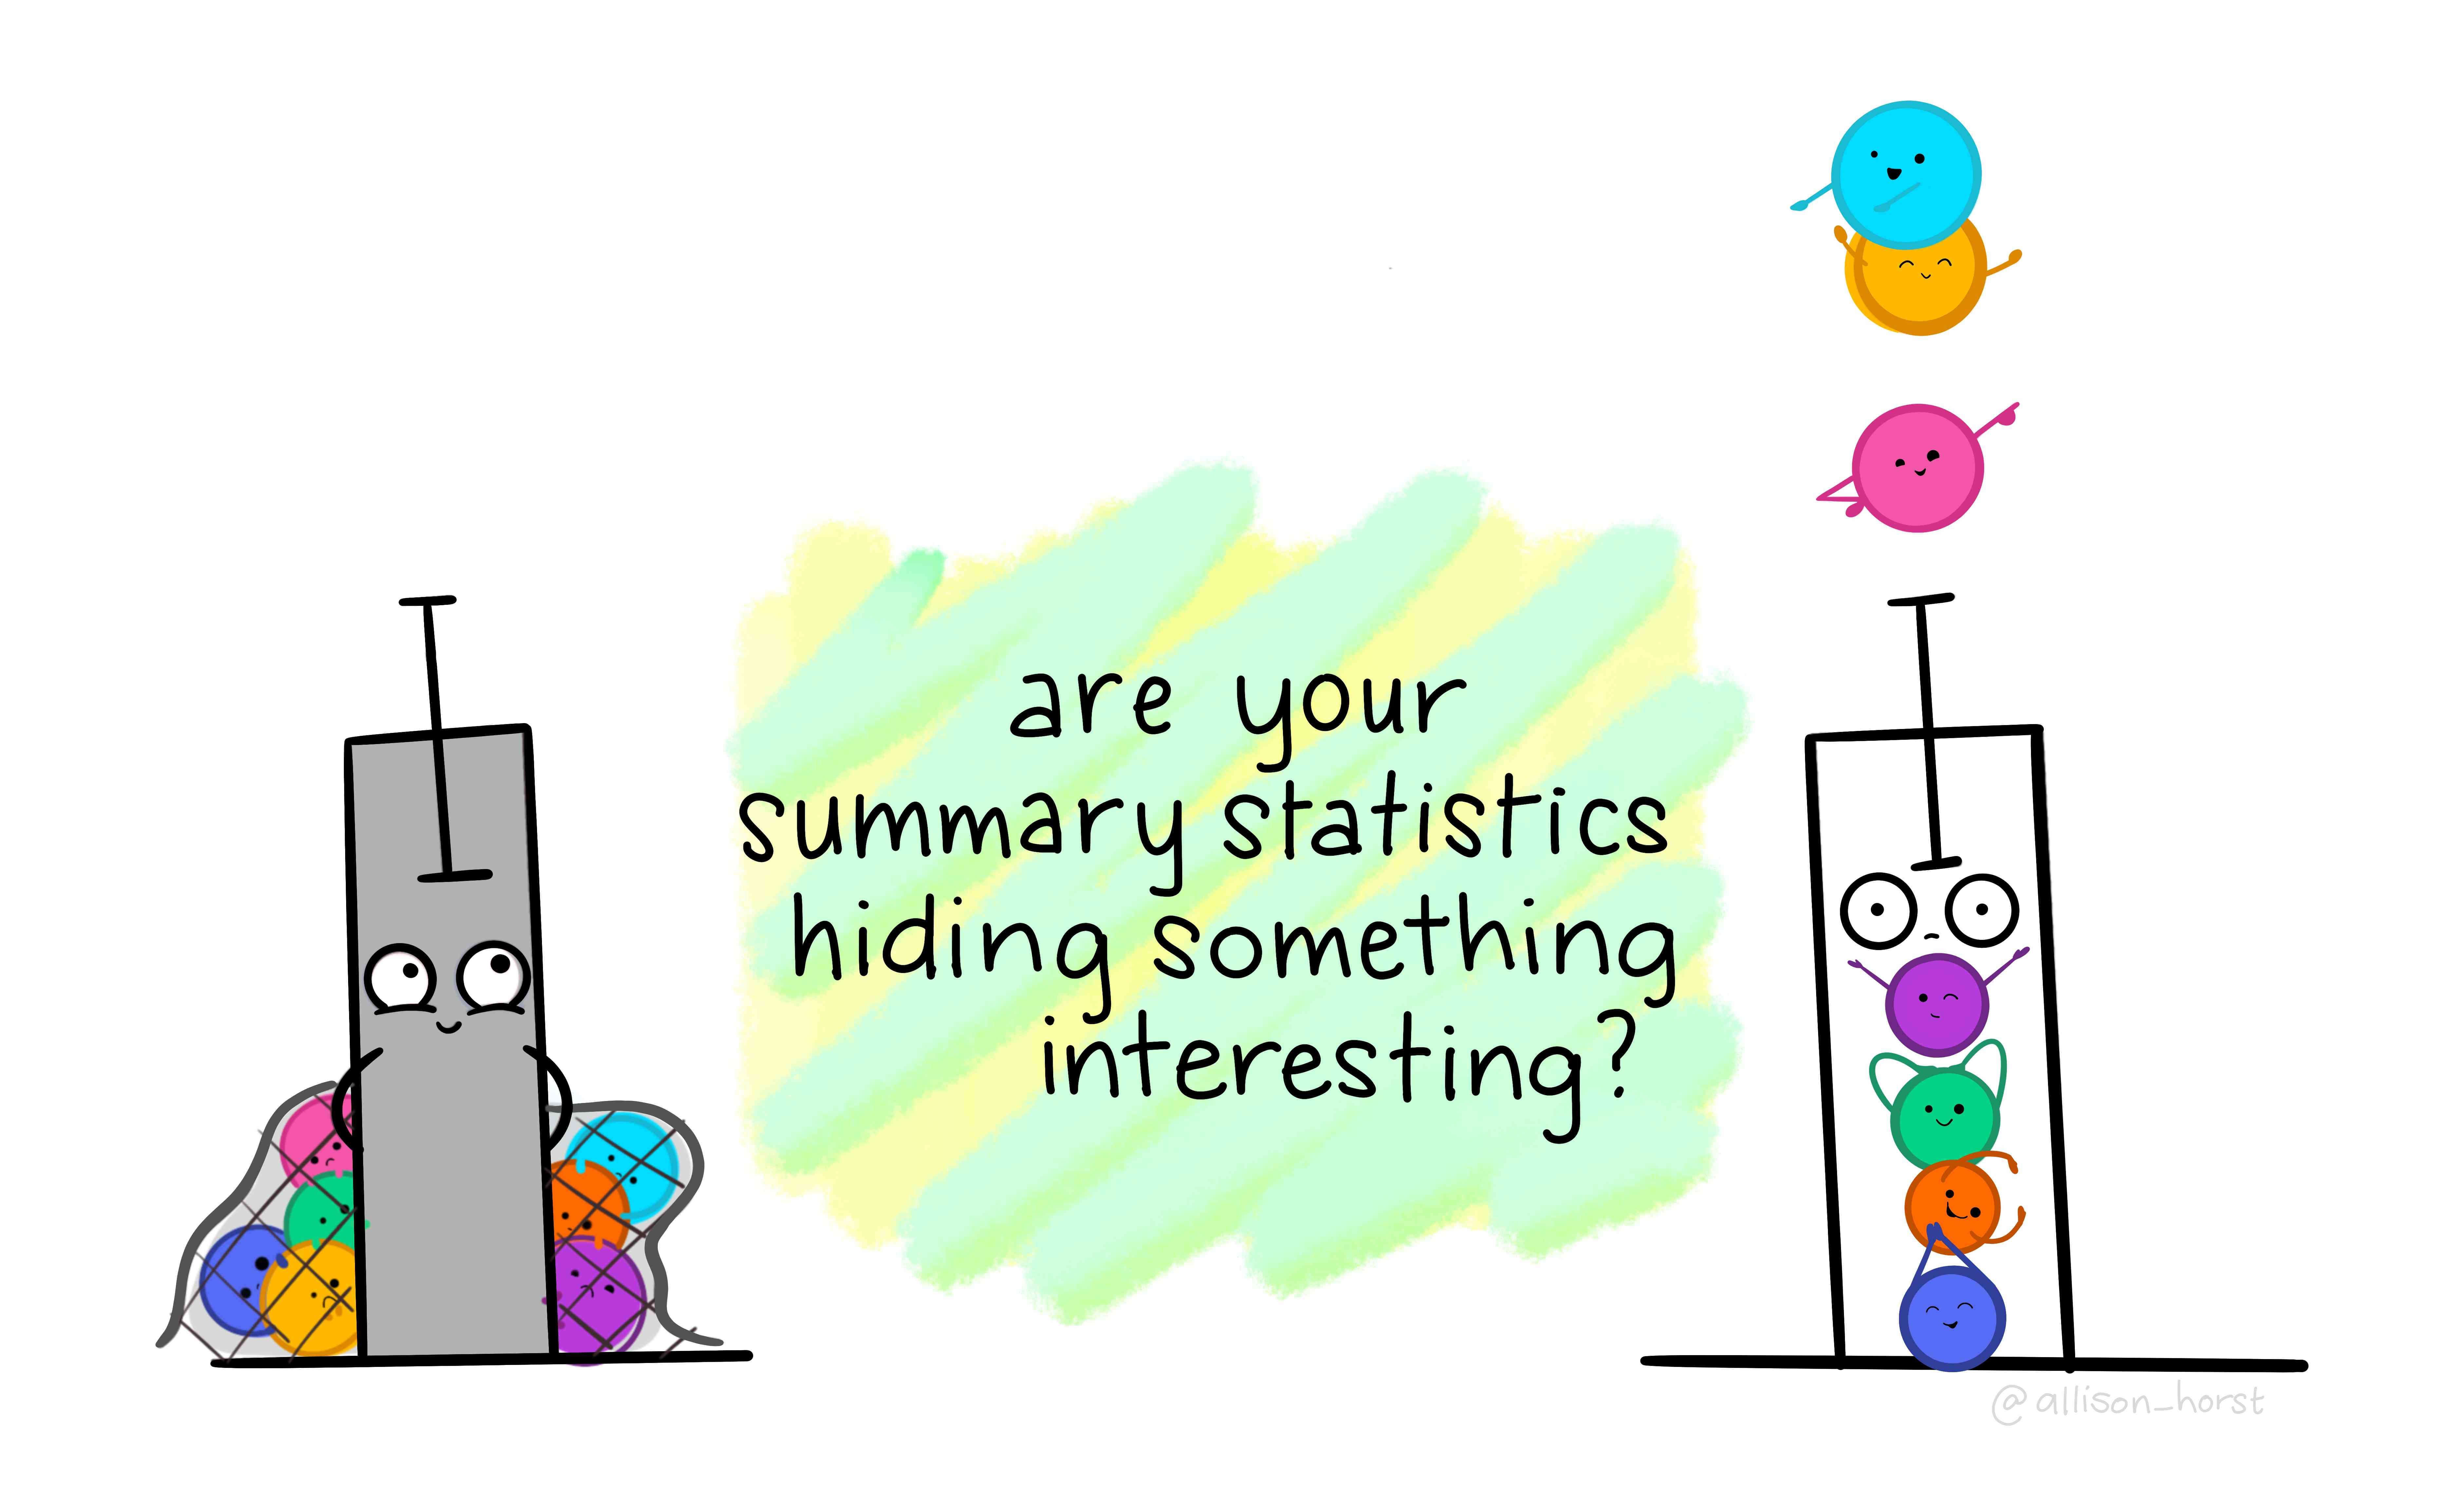
\includegraphics[width=1\linewidth]{./images/lab_3_summary_stats} \hfill{}

\caption{Exploratory analysis.}\label{fig:unnamed-chunk-47}
\end{figure}

To start exploring our data it essential to distinguish the adequate tools and measures available for the type of data in question. As you know now, there are two broad types: (1) categorical and (2) numeric.

There are several ways in which we can summarise our data. Today, we will use a useful package called \texttt{vtable}. Install it in your session running the following line from your console:

\begin{Shaded}
\begin{Highlighting}[]
\FunctionTok{install.packages}\NormalTok{(}\StringTok{\textquotesingle{}vtable\textquotesingle{}}\NormalTok{)}
\end{Highlighting}
\end{Shaded}

Once it is installed, make sure to load it with the next line. This time copy and paste it in your \texttt{R} script, so you can run it every time you restart your session.

\begin{Shaded}
\begin{Highlighting}[]
\FunctionTok{library}\NormalTok{(vtable)}
\end{Highlighting}
\end{Shaded}

\hypertarget{categorical-data}{%
\subsection{Categorical data}\label{categorical-data}}

A usual way to explore the categorical data is using contingency and proportion tables. The contingency tables include the count for each category while the proportion tables contain the count divided by the total number of observations.

Try to focus on the interpretation of the outputs in the following section. At this time, it is just optional to run the code shown.

Let's say we are interested in the data's break down by respondents' sex (called \texttt{rsex} in the dataset). We will use function \texttt{sumtable()} of the \texttt{vtable} package to produce a contingency table for a single variable (known as One-Way contingency table).

\begin{Shaded}
\begin{Highlighting}[]
\FunctionTok{sumtable}\NormalTok{(nilt\_subset, }\AttributeTok{vars =} \FunctionTok{c}\NormalTok{(}\StringTok{\textquotesingle{}rsex\textquotesingle{}}\NormalTok{))}
\end{Highlighting}
\end{Shaded}

\begin{table}

\caption{\label{tab:unnamed-chunk-50}Summary Statistics}
\centering
\begin{tabular}[t]{lll}
\toprule
Variable & N & Percent\\
\midrule
rsex & 1204 & \\
... Male & 537 & 45\%\\
... Female & 667 & 55\%\\
\bottomrule
\end{tabular}
\end{table}

From the result, we see that there are more female respondents than males.

Specifically, we see that males respondents represent 44.6\% of the total sample, whereas females 55.4\%.

We can do this with any type of categorical variable. Let's see how the sample is split by religion (\texttt{religcat}). So, we will add it to in the \texttt{vars} argument.

\begin{Shaded}
\begin{Highlighting}[]
\FunctionTok{sumtable}\NormalTok{(nilt\_subset, }\AttributeTok{vars =} \FunctionTok{c}\NormalTok{(}\StringTok{\textquotesingle{}rsex\textquotesingle{}}\NormalTok{, }\StringTok{\textquotesingle{}religcat\textquotesingle{}}\NormalTok{))}
\end{Highlighting}
\end{Shaded}

\begin{table}

\caption{\label{tab:unnamed-chunk-51}Summary Statistics}
\centering
\begin{tabular}[t]{lll}
\toprule
Variable & N & Percent\\
\midrule
rsex & 1204 & \\
... Male & 537 & 45\%\\
... Female & 667 & 55\%\\
religcat & 1168 & \\
... Catholic & 491 & 42\%\\
\addlinespace
... Protestant & 497 & 43\%\\
... No religion & 180 & 15\%\\
\bottomrule
\end{tabular}
\end{table}

As you can see, about the same number of people are identified as being catholic or protestant, and a relatively small number with no religion.

What if we want to know the religious affiliation break-down by males and females. This is where Two-Way contingency tables are useful and very common in quantitative research. To produce it, we have to specify the group argument in the \texttt{sumtable} function as following:

\begin{Shaded}
\begin{Highlighting}[]
\FunctionTok{sumtable}\NormalTok{(nilt\_subset, }\AttributeTok{vars =} \FunctionTok{c}\NormalTok{(}\StringTok{\textquotesingle{}religcat\textquotesingle{}}\NormalTok{), }\AttributeTok{group =} \StringTok{\textquotesingle{}rsex\textquotesingle{}}\NormalTok{)}
\end{Highlighting}
\end{Shaded}

\begin{table}

\caption{\label{tab:unnamed-chunk-52}Summary Statistics}
\centering
\begin{tabular}[t]{lllll}
\toprule
\multicolumn{1}{c}{rsex} & \multicolumn{2}{c}{Male} & \multicolumn{2}{c}{Female} \\
\cmidrule(l{3pt}r{3pt}){1-1} \cmidrule(l{3pt}r{3pt}){2-3} \cmidrule(l{3pt}r{3pt}){4-5}
Variable & N & Percent & N & Percent\\
\midrule
religcat & 520 &  & 648 & \\
... Catholic & 209 & 40\% & 282 & 44\%\\
... Protestant & 211 & 41\% & 286 & 44\%\\
... No religion & 100 & 19\% & 80 & 12\%\\
\bottomrule
\end{tabular}
\end{table}

There are some interesting results from this table. You can see that there are proportionally more female respondents who are either Catholic or Protestant than males, namely 43.5\% vs 40.2\% and 44.1\% vs 40.6\%, respectively. We also see that there are almost 20\% of male respondents who do not self-identify with a religion which contrast to the 12\% of female participants.

\hypertarget{activity-1-1}{%
\subsection{Activity 1}\label{activity-1-1}}

From your R Studio Cloud script, do the following activities using the data in the \texttt{nilt\_subset} object (feel free to copy and adapt the code shown above):

\begin{itemize}
\tightlist
\item
  Create a One-Way contingency table for \texttt{uninatid} in the \texttt{nilt\_subset} dataset using the \texttt{sumtable()} function;
\item
  Using the variables \texttt{religcat} and \texttt{uninatid}, generate a Two-Way contingency table;
\item
  Are your summary statistics hiding something interesting? Discuss your results with your neighbour or your tutor.
\end{itemize}

\hypertarget{continuous-numeric-data}{%
\subsection{Continuous (numeric) data}\label{continuous-numeric-data}}

In the previous section we've learnt how to summarise categorical data. But very often we want to work with continuous numeric variables or a combination of both. To summarise and understand numeric data there are two main types: \emph{measures of centrality} and \emph{measures of spread}.

As before, try to focus on the interpretation of the outputs in the following section. At this time, it is just optional to run the code shown.

\hypertarget{measures-of-centrality}{%
\subsubsection{Measures of centrality}\label{measures-of-centrality}}

In quantitative research, we usually have access to many observations in a sample which contains different attributes for each of them. It would be difficult (and probably not very useful) to talk about each of the NILT respondents one by one. Instead, to describe this sample we need measures that roughly represent all participants.

This is actually an important step in quantitative research, since it allows us to characterise the people that we are studying. For example, in the previous section we only talked about the respondents' sex and political affiliation, but who are the people we are talking about? Probably a place to start digging deeper is to know their age. The first tool that we will use to understand numeric values is a histogram. Let's see how the age of NILT respondents is distributed.

\begin{Shaded}
\begin{Highlighting}[]
\FunctionTok{hist}\NormalTok{(nilt\_subset}\SpecialCharTok{$}\NormalTok{rage)}
\end{Highlighting}
\end{Shaded}

\begin{flushleft}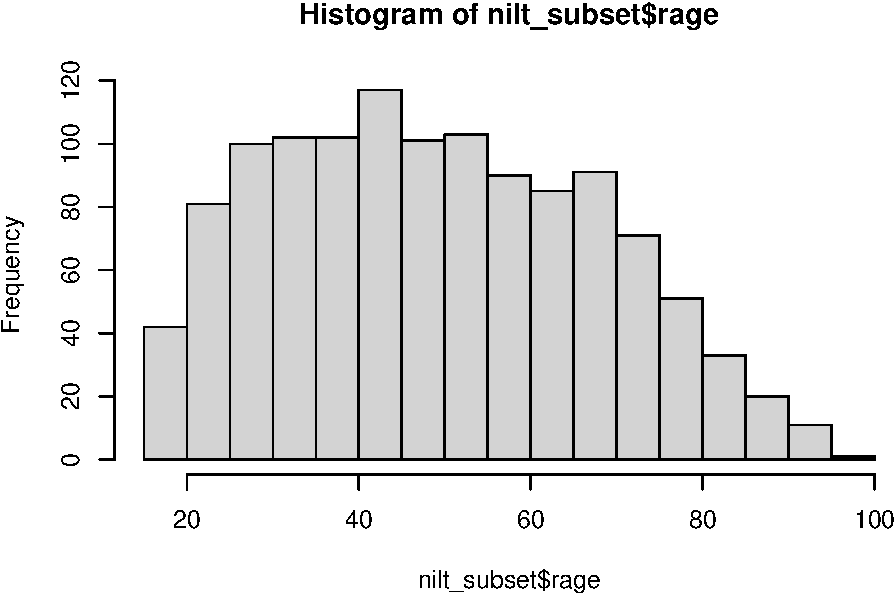
\includegraphics[width=1\linewidth]{lab-workbook_files/figure-latex/unnamed-chunk-53-1} \end{flushleft}

This plot show us on the X axis (horizontal) the age and the frequency on the Y axis. We can see that the youngest age in the sample is somewhere close to 20, and the oldest is almost 100. We also observe that the total number of observations (represented by the frequency on the vertical axis) for extreme values (close to 20 on the left-hand side and 100 on the right-hand side), tends to be lower than the values in the centre of the plot (somewhere between 30 and 45). For instance, we can see that there are approximately 120 respondents who are around 40 years old, that seems to be the most \emph{popular}/frequent age in our sample. Now, we can represent these central values with actual measures, typically \emph{mean} or \emph{median}.

The \emph{median} is the mid-point value in a numeric series. If you sort the values and split it by half, the value right in the middle is the median. Luckily there is a function ready to be used called\ldots{} You guessed it - \texttt{median()}.

\begin{Shaded}
\begin{Highlighting}[]
\FunctionTok{median}\NormalTok{(nilt\_subset}\SpecialCharTok{$}\NormalTok{rage, }\AttributeTok{na.rm =} \ConstantTok{TRUE}\NormalTok{)}
\end{Highlighting}
\end{Shaded}

\begin{verbatim}
## [1] 48
\end{verbatim}

The median age is 48, that means that 50\% (or half) of the respondents are equal or younger than this, and the other 50\% is equal or older.\footnote{Note that the argument \texttt{na.rm} equal \texttt{TRUE} is used in the function. The `na' bit refers to missing values, and the `rm' refers to remove. So we are telling R to remove the missing values when computing the median. This is because we do not know the age of 3 of the respondents in the sample.}

To compute the \emph{mean} manually, we need to sum all our values and divide it by the total number of the observations as follows:
\[ mean =\frac{  x_1 + x_2 + x_3 ...+x_n } {n} \]
The formula above is for you to know that this measure considers the magnitude of all values included in the numeric series. Therefore, the average is sensitive to extreme numbers (e.g.~a very very old person). To compute the mean you need the \texttt{mean()} function.

\begin{Shaded}
\begin{Highlighting}[]
\FunctionTok{mean}\NormalTok{(nilt\_subset}\SpecialCharTok{$}\NormalTok{rage, }\AttributeTok{na.rm =}\NormalTok{ T)}
\end{Highlighting}
\end{Shaded}

\begin{verbatim}
## [1] 49.61532
\end{verbatim}

As you can see, the above measures try to approximate values that fall somewhere in the centre of the histogram plot, and represent all observations in the sample. They tell different things and are sometimes more (or less) suitable in a specific situation.

\hypertarget{measures-of-spread}{%
\subsubsection{Measures of spread}\label{measures-of-spread}}

By contrast, there are measures that helps us to describe how far away a series of numeric values are from the centre. The common measures of spread are \emph{quartiles}, \emph{variance} and \emph{standard deviation}.

The quartiles are very useful to quickly see how numeric data is distributed. Imagine that we sort all ages in the sample and split it in four equal parts. The first quartile includes the lowest 25\% values, the second the other 25\%, the third other other 25\%, and the fourth the highest 25\%. To compute quartiles we can use the \texttt{quantile} function.

\begin{Shaded}
\begin{Highlighting}[]
\FunctionTok{quantile}\NormalTok{(nilt\_subset}\SpecialCharTok{$}\NormalTok{rage, }\AttributeTok{na.rm =}\NormalTok{ T)}
\end{Highlighting}
\end{Shaded}

\begin{verbatim}
##   0%  25%  50%  75% 100% 
##   18   35   48   64   97
\end{verbatim}

In our sample, the youngest quarter of the respondents is between 18 and 35 years old. The second quarter is between 35 and 48 years old. The next quartile is between 48 and 64. The oldest 25\% of the respondents is between 64 and 97.

The \emph{variance} is useful to obtain a singe measure of spread (instead of four values, as the above) taking the mean as a reference. This is given by the following formula:

\[ var = \frac{ \sum(x - \bar{x})^2 }{n-1 } \]

To decipher the formula above, the \(\bar{x}\) represents the mean, the \(x\) represents each of the values in the numeric series. The formula takes each of the \(x\) values and subtract it from the \emph{mean} \(\bar{x}\). Later, it squares the result of the subtraction (that is multiply it by itself). This is done to obtain a positive value, since some numbers in the series will be lower than the mean (resulting in negative values). Then, we sum all of them and divide the sum by the size/length of the numeric sequence \(n\) minus 1. To estimate the variance in R we only need the \texttt{var()} function.

\begin{Shaded}
\begin{Highlighting}[]
\FunctionTok{var}\NormalTok{(nilt\_subset}\SpecialCharTok{$}\NormalTok{rage, }\AttributeTok{na.rm =}\NormalTok{ T)}
\end{Highlighting}
\end{Shaded}

\begin{verbatim}
## [1] 343.3486
\end{verbatim}

As you can see, the result is not very intuitive. That is because we squared the subtraction. Luckily, there is a measure that put it in \emph{readable} scale. This is the \emph{standard deviation}. In essence this takes the square root of the variance (the reversed operation of squaring it):
\[sd=\sqrt{var}\]

To compute it in \texttt{R}, use the \texttt{sd()} function.

\begin{Shaded}
\begin{Highlighting}[]
\FunctionTok{sd}\NormalTok{(nilt\_subset}\SpecialCharTok{$}\NormalTok{rage, }\AttributeTok{na.rm =}\NormalTok{ T)}
\end{Highlighting}
\end{Shaded}

\begin{verbatim}
## [1] 18.52967
\end{verbatim}

This measure is more \emph{human readable} than the variance. Don't worry too much about the formula. An important thing to remember is what the measure represents. An informal definition of the standard deviation is \emph{the average distance from the mean}. In essence, it tell us how far the values in our data are from the mean.

\hypertarget{putting-it-all-together}{%
\subsection{Putting it all together}\label{putting-it-all-together}}

Phew, that was a lot!\ldots{}

\ldots{} Luckily we can use the \texttt{sumtable} function to compute all these measures at the same time!

It is very simple. You can compute a quick summary for age as following:

\begin{Shaded}
\begin{Highlighting}[]
\FunctionTok{sumtable}\NormalTok{(nilt\_subset, }\AttributeTok{vars =} \FunctionTok{c}\NormalTok{(}\StringTok{\textquotesingle{}rage\textquotesingle{}}\NormalTok{))}
\end{Highlighting}
\end{Shaded}

\begin{table}

\caption{\label{tab:unnamed-chunk-59}Summary Statistics}
\centering
\begin{tabular}[t]{llllllll}
\toprule
Variable & N & Mean & Std. Dev. & Min & Pctl. 25 & Pctl. 75 & Max\\
\midrule
rage & 1201 & 50 & 19 & 18 & 35 & 64 & 97\\
\bottomrule
\end{tabular}
\end{table}

The result displays the number of observations used (N), the mean, the standard deviation, minimum, the 1st (same as `Pctl. 25') and 3rd quartile (same as `Pctl. 75'), as well as the maximum (i.e., eldest respondent).

\hypertarget{categorical-and-numeric-data}{%
\subsubsection{Categorical and numeric data}\label{categorical-and-numeric-data}}

Lastly, there will be times in which you will need to compute a summary combining categorical and numeric data, to compare groups for example. The good news is that we can use exactly the same function and syntax to do this. Let's take the following example to compute the summary of the respondent's age (\texttt{rage}) by gender:

\begin{Shaded}
\begin{Highlighting}[]
\FunctionTok{sumtable}\NormalTok{(nilt\_subset, }\AttributeTok{vars =} \FunctionTok{c}\NormalTok{(}\StringTok{\textquotesingle{}rage\textquotesingle{}}\NormalTok{), }\AttributeTok{group =} \StringTok{\textquotesingle{}rsex\textquotesingle{}}\NormalTok{)}
\end{Highlighting}
\end{Shaded}

\begin{table}

\caption{\label{tab:unnamed-chunk-60}Summary Statistics}
\centering
\begin{tabular}[t]{lllllll}
\toprule
\multicolumn{1}{c}{rsex} & \multicolumn{3}{c}{Male} & \multicolumn{3}{c}{Female} \\
\cmidrule(l{3pt}r{3pt}){1-1} \cmidrule(l{3pt}r{3pt}){2-4} \cmidrule(l{3pt}r{3pt}){5-7}
Variable & N & Mean & SD & N & Mean & SD\\
\midrule
rage & 535 & 51 & 18 & 666 & 49 & 19\\
\bottomrule
\end{tabular}
\end{table}

In the code above, we are simple specifying the variable \texttt{rage} and grouping the summary by \texttt{rsex}. This produces a small summary included the number of observations in each category an the main measure of centrality and spread, namely the mean and the std. dev.

\hypertarget{activity-2-1}{%
\subsection{Activity 2}\label{activity-2-1}}

Can money buy happiness?

Using the data in the \texttt{nilt\_subset} dataset, complete the following activities. This will be a good practice run for doing the research report when you run your own analysis on the NILT teaching dataset. Handy!

\begin{itemize}
\tightlist
\item
  Using the \texttt{hist()} function plot a histogram of personal income \texttt{persinc2}. From the NILT documentation this variable refers to annual personal income in £ before taxes and other deductions (use the \texttt{\$} symbol after the name of the dataset and then the name of the variable inside the function);
\item
  Create a summary of the personal income \texttt{persinc2} variable, using the \texttt{sumtable()} function;
\item
  Finally, compute the mean and standard deviation of the personal income \texttt{persinc2}, grouped by happiness \texttt{ruhappy}. What do you observe?
\item
  Discuss the results with your neighbour or your tutor.
\end{itemize}

\hypertarget{reporting-in-r-markdown}{%
\chapter{Reporting in R Markdown}\label{reporting-in-r-markdown}}

\hypertarget{introduction}{%
\section{Introduction}\label{introduction}}

In the previous labs you were exploring the 2012 \href{https://www.ark.ac.uk/nilt/}{Northern Ireland Life and Times Survey (NILT)}. You've learnt how to download, read and format the data. Also, you've learnt how to explore categorical and numeric data and a mix of them. In this lab, you will learn about how to efficiently report quantitative results directly from R, using R Markdown, which is used by many academics and professionals in a workplace setting to communicate quantitative findings to a wider audience. R Markdown is also what you will use to write your research report assignment for this course. So, Let's dive in and learn more!

\hypertarget{r-markdown}{%
\section{R Markdown}\label{r-markdown}}

R Markdown (Rmd) is a \textbf{different} type of file included in R Studio (and it is actually a different programming language). This allows you to generate reports in common file types, such as \texttt{.html} (the same one used for this lab workbook you're reading right now), \texttt{.pdf} or word (\texttt{.doc}). The interesting thing is that the Rmd file allows you to integrate text, code, and plots directly into your report (so you do not have to copy and paste tables or graphs into a Word document, for example, which is often very messy and time-consuming). You have already seen how well this works in the lab workbooks so far, which are written entirely in R Markdown.

The basic components of an Rmd file are: the \textbf{\emph{code}}, \textbf{\emph{text}} and \textbf{\emph{metadata}}. The code is integrated by blocks called `chunks', and the metadata contains information to format the report. We believe the best way to learn is by doing it. So, let's create your first Rmd document!

\hypertarget{first-r-markdown-document}{%
\subsection{First R Markdown document}\label{first-r-markdown-document}}

We will continue working in the same project called \emph{NILT} in \href{https://rstudio.cloud/}{RStudio Cloud}.

\begin{enumerate}
\def\labelenumi{\arabic{enumi}.}
\tightlist
\item
  Please go to your `Quants lab group' in \href{https://rstudio.cloud/}{RStudio Cloud} (log in if necessary);
\item
  Open your own copy of the `NILT' project from the `Quants lab group';
\item
  Create a new Rmd file, this is similar as creating and \texttt{R\ Script}, from the `File' tab on the top-left: \texttt{File\textgreater{}New\ File\textgreater{}R\ Markdown...} (Rstudio may ask to install some packages, click `Yes');
\item
  Type `Test1' in `Tile' section and your name in the `Author' box. Leave the `Default Output Format' as \texttt{HTML}. Then, click `OK'.
\item
  Save the Rmd file clicking on \texttt{File\textgreater{}Save\ as...}, type \texttt{Test1} in the `File name' box, and click on the Save button.
\end{enumerate}

After completing the previous steps, your screen should look like this (You can minimize the console to expand pane 1):

\begin{figure}

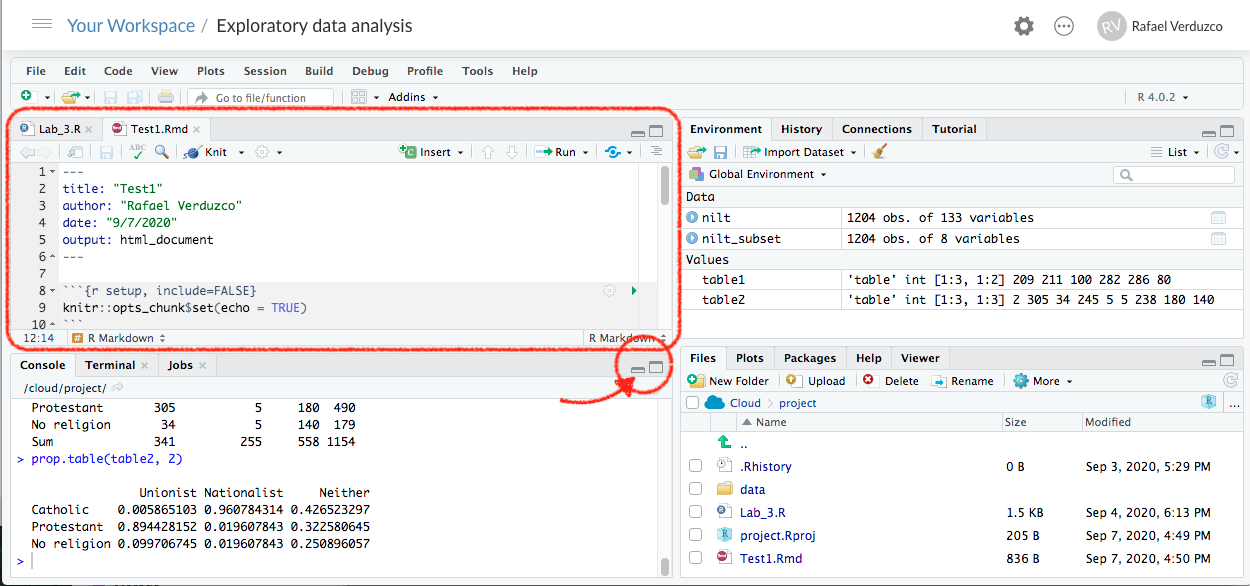
\includegraphics[width=1\linewidth]{./images/lab4_rmd_view} \hfill{}

\caption{Rmd file.}\label{fig:rmd-file}
\end{figure}

Note that now you have two files open in Pane 1, one tab includes the \texttt{R} script that we created in the last lab (called \texttt{Lab\_3.R}), and the other is the \texttt{Rmd} document that you just created.

The Rmd document \texttt{Test1} contains an example by default. The first bit on the top enclosed by the dashes \texttt{-\/-\/-}, contains the general metadata to format the output, as shown in the Figure \ref{fig:yaml-chunk}. This bit is called YAML. In the default example, it contains the title, name of the author, data and the type of output (html). You can adjust this information directly by typing the relevant info (e.g.~date or name).

\begin{figure}

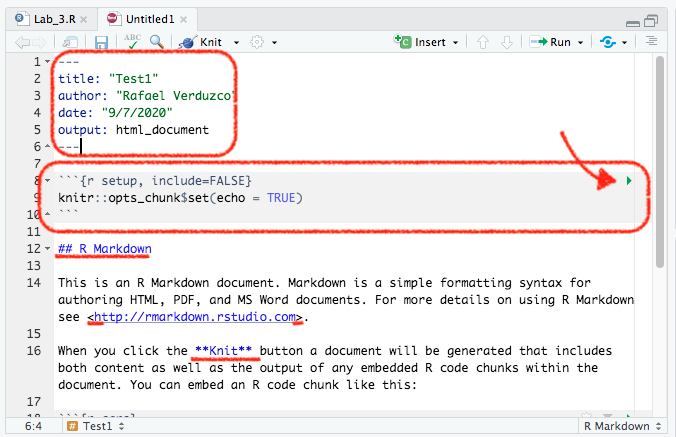
\includegraphics[width=1\linewidth]{./images/lab4_rmd_view_2} \hfill{}

\caption{YAML and code chunk.}\label{fig:yaml-chunk}
\end{figure}

Below the YAML shown in Figure \ref{fig:yaml-chunk}, there is another box. This is an \texttt{R} code `chunk'. To run a chunk of code individually (that is to visualize a partial result of an \texttt{Rmd} document), you can click on the green arrow pointed on the top-left of the first chunk.

In line 12, you have a second-level header, which contains the name of a section in the document. As you can see this is preceded by double hash tag \texttt{\#\#}. If you want a first-level header section, you would require only one hash tag like this \texttt{\#}, and three for a third-level header. Finally the `Knit' word is enclosed by double asterisk \texttt{**}. This is to format the characters enclosed in bold.

In line 26, you will see a chunk including a basic plot. Let's check the results that this example in `Test1' produce.

To render the document from Rmd to HTML, we need to \emph{Knit} it by clicking on the icon shown below. Try it!

\begin{figure}
\centering
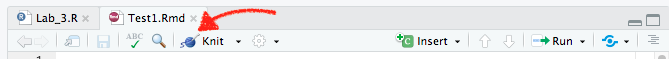
\includegraphics{./images/lab4_rmd_knit.png}
\caption{Knit button}
\end{figure}

RStudio may ask you if you want to update some packages, click `Yes'.

After you knit the document, a window with the output will pop-up automatically. As you can see, this document contains the main title, followed by your name and date, as specified in the YAML. After, there is a second-level header which includes the first section of this example document. Also the the word `Knit' is shown in bold, as it was wrapped by double asterisk \texttt{**}.

An interesting thing is that we can integrate the result of our code in the output as we did with the second chunk (which starts in line 18). Here, we can use a summary of the data set \texttt{cars} (which is an in-built data set in \texttt{R} that contains only two variables).

Similarly, you can create a \texttt{.pdf} file. To do this, instead of clicking on on the \emph{Knit} icon directly, click on the black arrow next to it. Then click `Knit to PDF'. Try it and see the result.

When you knitted the document, R Studio actually created a new \texttt{.html} or \texttt{.pdf} file named as same as your Rmd document. You can confirm this in the `File' tab in Pane 4. You can to download this file from the cloud to your local drive by clicking on the box of the output file. Then, click \texttt{More\textgreater{}Export...} in the same pane (or clicking on the gear icon in pane 4).

\textbf{IMPORTANT}: Rmd files are different from simple R scripts. While everything you write in an R script is interpreted as code, only the bits within the code chunks will be interpreted as code in Rmd files. Everything else not within chunks in an Rmd file is interpreted as text.

\hypertarget{activity-5}{%
\section{Activity}\label{activity-5}}

In the \texttt{Test1.Rmd} file that you just created, do the following:

\begin{itemize}
\tightlist
\item
  Change the title of the document in the YAML to `My first R Markdown document'.
\item
  In the code chunk in line 21, replace the existing line (\texttt{summary(car)}) with the following: \texttt{glimpse(iris)}.
\item
  In the code chunk called `pressure', change \texttt{echo=FALSE} to \texttt{echo=TRUE}.
\item
  At the very bottom of the script, create a new paragraph and write one or two lines briefly describing how you think quantitative methods are improving your discipline (e.g.~politics, sociology, social and public policy, or central and eastern European studies).
\item
  Knit the document in \texttt{html} format.
\item
  Download the newly edited version of the \texttt{Test1.html} document to your machine.
\item
  Discuss how each of the edits suggested above modify the output with your neighbour or your tutor.
\end{itemize}

Make sure you've got the basics of R Markdown, since this is the tool which you will use to write your final assignment (i.e.~research report). If there is something not very clear, or you are curious about, feel free to ask your tutor. They will be happy to answer your questions.

\hypertarget{visual-exploratory-analysis}{%
\chapter{Visual exploratory analysis}\label{visual-exploratory-analysis}}

\hypertarget{introduction-1}{%
\section{Introduction}\label{introduction-1}}

In this lab, we will extend your skills to explore data by visualizing it\ldots and \texttt{R} is great for this! It is actually a highly-demanded skill in the job market.

Visualizing data is an important process in at least two stages in quantitative research: First, for your as a researcher to get familiar with the data; and second, to communicate your findings. \texttt{R} includes two important tools to achieve this: First, the \texttt{ggplot2} package (included in \texttt{tidyverse}), a powerful tool to explore and plot data. Second, \href{https://rmarkdown.rstudio.com/}{R Markdown} which allows you to create integrated quantitative reports. Combining and mastering the two can create very effective results.

\hypertarget{data-visualization}{%
\section{Data visualization}\label{data-visualization}}

Visual data exploration with \texttt{ggplot2} (Artwork by @alison\_horst).

\begin{figure}

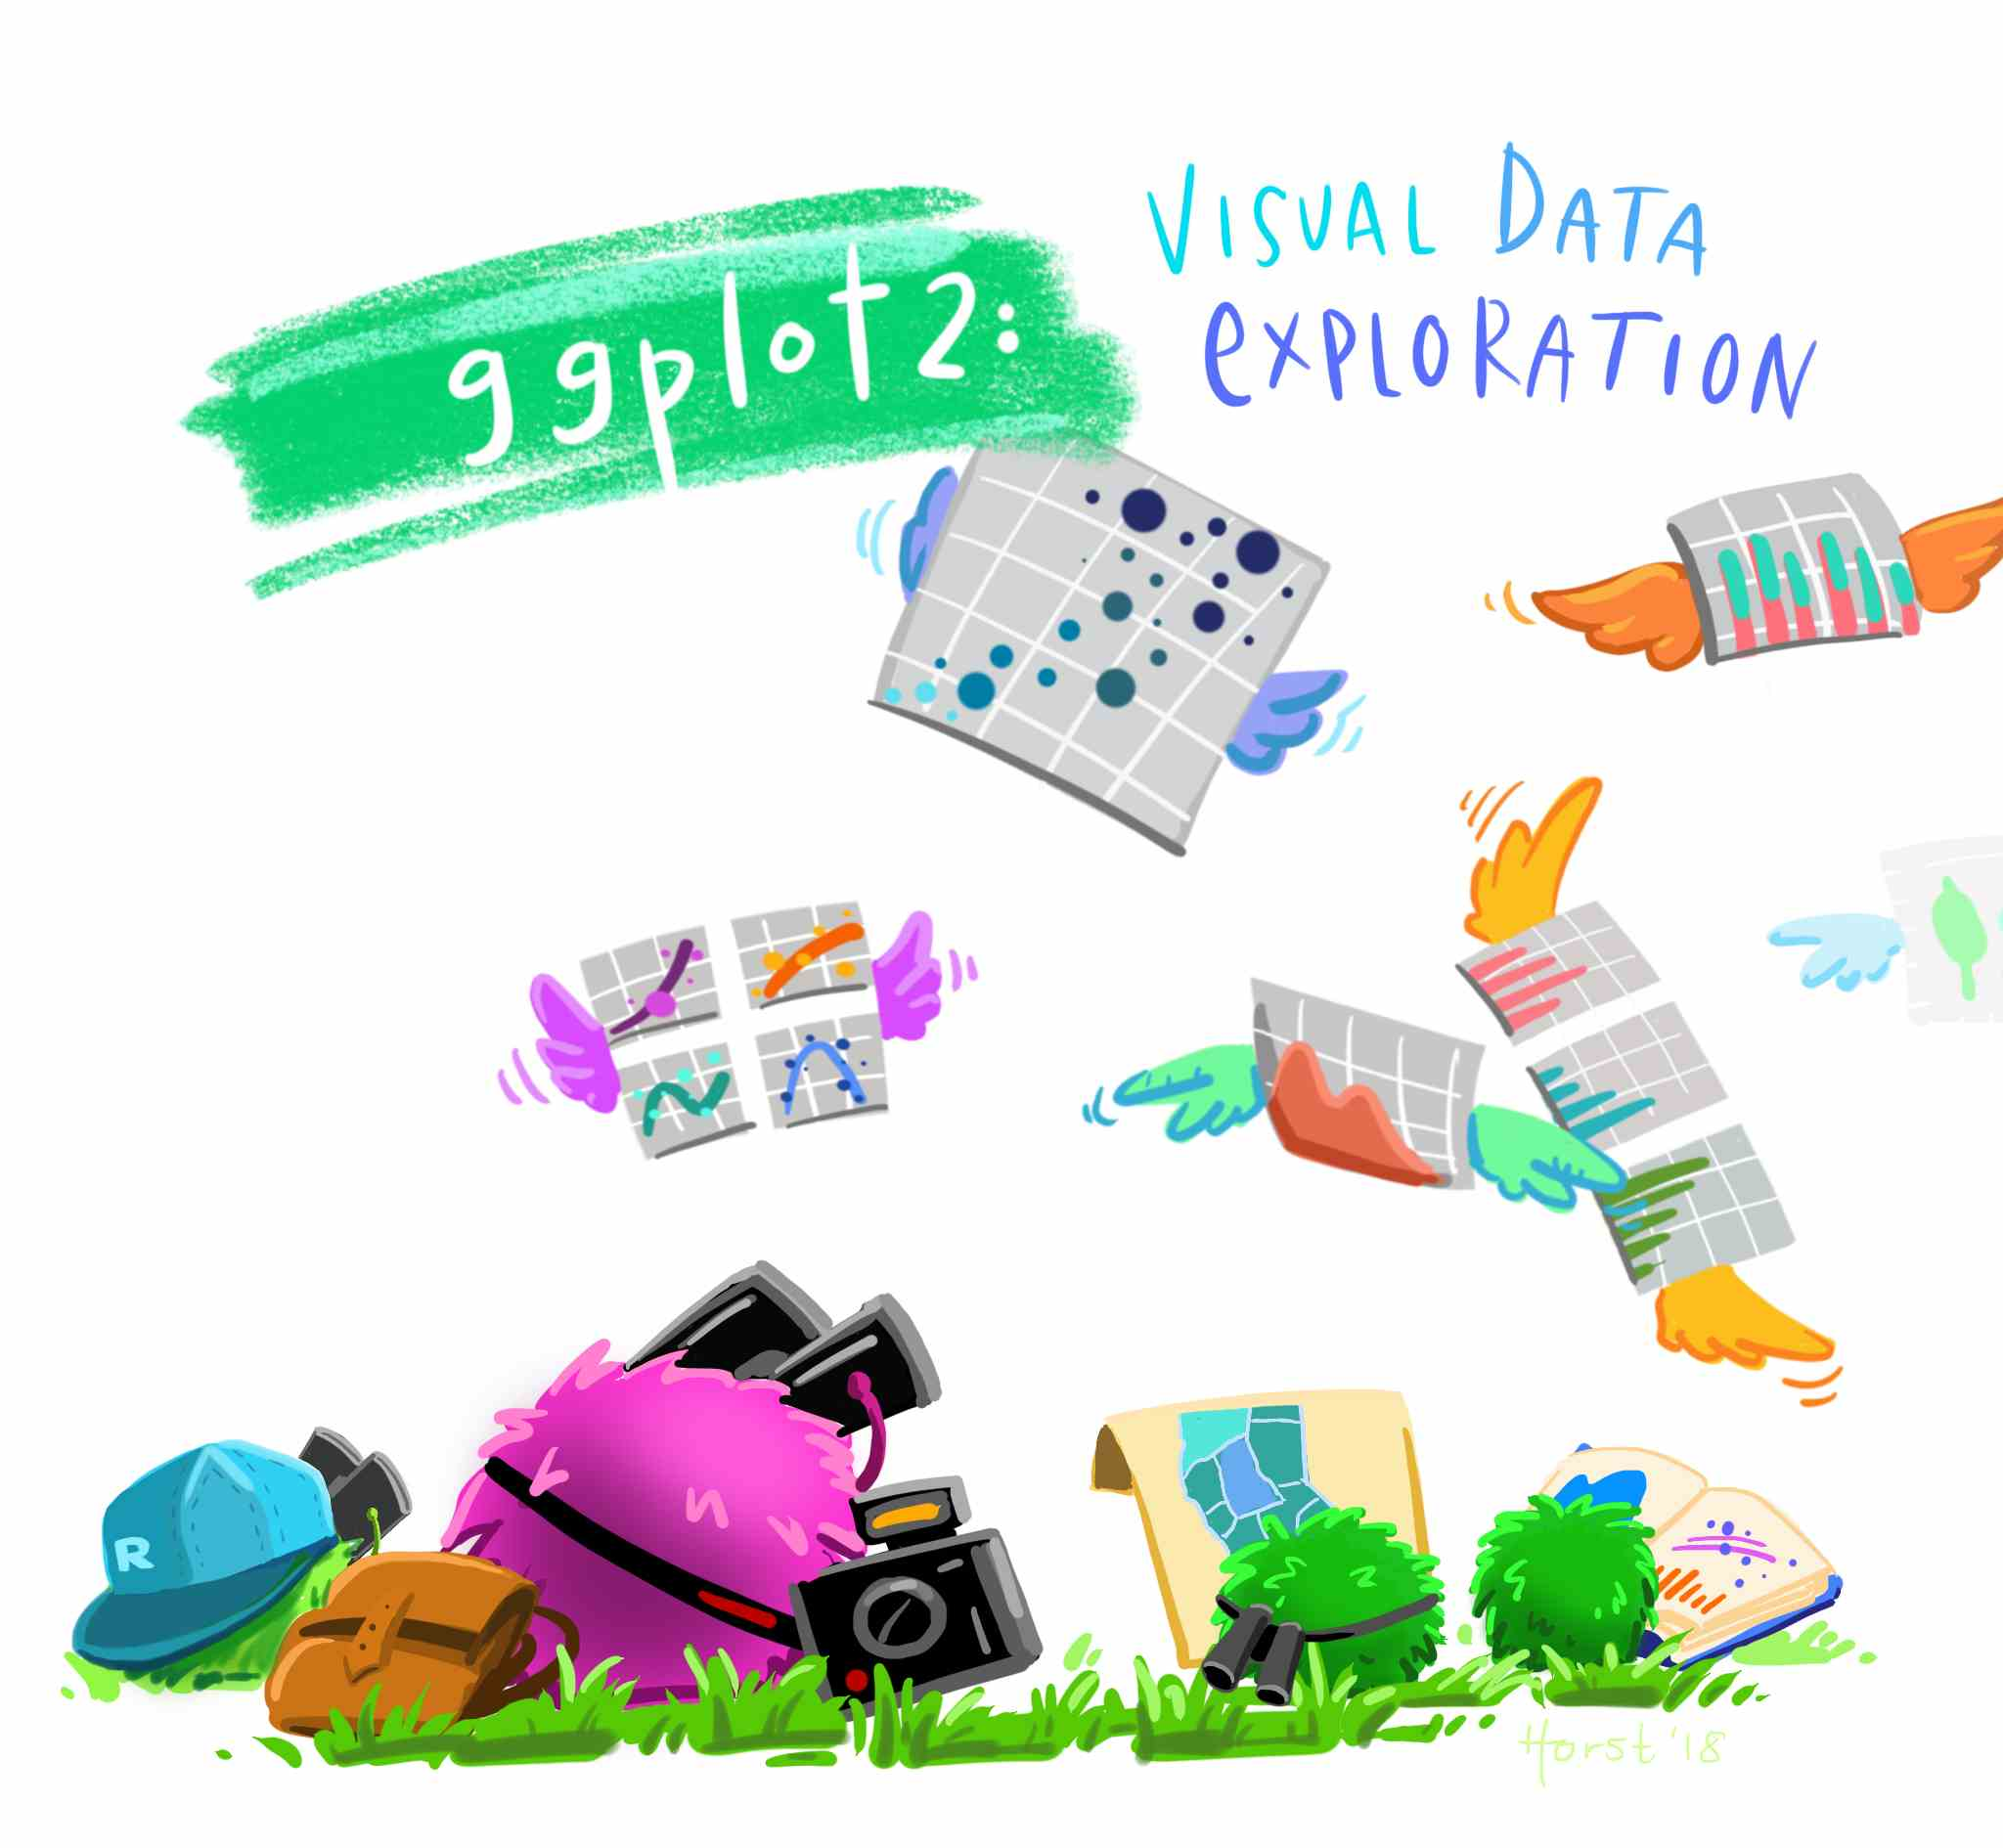
\includegraphics[width=1\linewidth]{./images/lab4_ggplot2_exploratory} \hfill{}

\caption{Visual data exploration. Source: @Horst}\label{fig:unnamed-chunk-61}
\end{figure}

Different plot types serve different types of data. In the last lab, we introduced some functions to summarise your data and to generate summaries for specific types of variable. This will help you to decide what the most suitable plot is for your data or variable. The table below presents a minimal guide to choose the type of plot as a function of the type of data you intend to visualize. In addition, it splits the type of plot by the number of variables included in the visualization, one for \emph{univariate}, or two for \emph{bivariate}. Bivariate plots are useful to explore the relationship between variables.

\begin{longtable}[]{@{}lll@{}}
\toprule\noalign{}
& \textbf{Univariate} & \textbf{Bivariate} \\
\midrule\noalign{}
\endhead
\bottomrule\noalign{}
\endlastfoot
\textbf{Categorical} & Bar plot / Pie chart & Bar plot \\
\textbf{Numeric} & Histogram / boxplot & Scatter plot \\
\textbf{Categorical} + \textbf{Numeric} & - & Box plot \\
\end{longtable}

\hypertarget{prepare-the-rmd-document-and-data}{%
\subsection{Prepare the Rmd document and data}\label{prepare-the-rmd-document-and-data}}

As we did in the last session, let's learn by doing. We will continue working in the same project called \emph{NILT} in \href{https://rstudio.cloud/}{RStudio Cloud}. Set up your session as follow:

\begin{enumerate}
\def\labelenumi{\arabic{enumi}.}
\tightlist
\item
  Go to your `Quants lab group' in \href{https://rstudio.cloud/}{RStudio Cloud} (log in if necessary);
\item
  Open your own copy of the `NILT' project from the `Quants lab group';
\end{enumerate}

Next, create a new Rmd document following the next steps.

\begin{enumerate}
\def\labelenumi{\arabic{enumi}.}
\tightlist
\item
  Create a new Rmd file titled `Lab 6. Data visualization', and write your name in the `Author' space.
\item
  Save the Rmd file clicking on \texttt{File\textgreater{}Save\ as...}, using \texttt{Lab\_6} in the `File name' box, and click on the `Save' button.
\item
  Delete all the contents in the default example with the exception of the first bit which contains the YAML and the first code chunk (that is keeping from line 1 to 10 and deleting everything from line 11).
\item
  In the setup chunk (line 8), change \texttt{echo} from \texttt{TRUE} to \texttt{FALSE} (this will hide the code for all chunks in the output).
\end{enumerate}

Once your Rmd document is ready, insert a new \texttt{R} code chunk. To do this, click on the `Insert' button on pane 1, and then click on `R'. This will insert an R code chunk as the ones we explored in `Test1'.

\begin{figure}

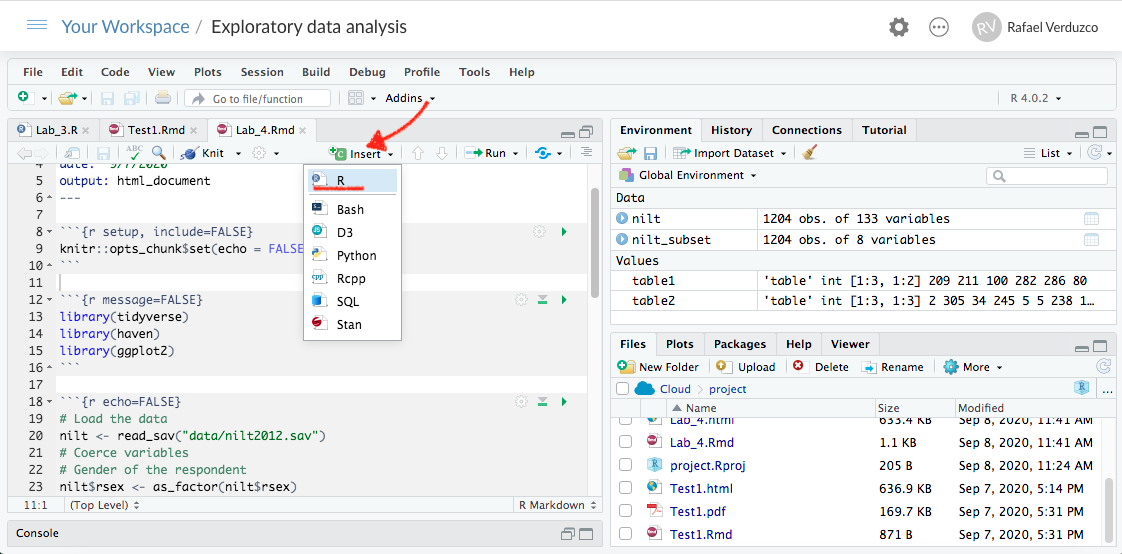
\includegraphics[width=1\linewidth]{./images/Lab4_chunk} \hfill{}

\caption{Insert a code chunk.}\label{fig:unnamed-chunk-62}
\end{figure}

In the body of the first chunk, load the packages that you will need. For now, it will be only \texttt{tidyverse}.

\begin{Shaded}
\begin{Highlighting}[]
\FunctionTok{library}\NormalTok{(tidyverse)}
\end{Highlighting}
\end{Shaded}

After the previous, insert a second chunk. In the body of the code copy and paste the lines below. This is to load the data we downloaded and formatted in the last lab in R format using the \texttt{readRDS()} function (note that we are reading the \texttt{.rds} file and not the original \texttt{.sav} file). Also, we will create a subset called \texttt{nilt\_subset} selecting only the variables that we are interested in for now, as we did in the previous lab.

\begin{Shaded}
\begin{Highlighting}[]
\CommentTok{\# Load the data from the .rds file we created in the last lab}
\NormalTok{nilt }\OtherTok{\textless{}{-}} \FunctionTok{readRDS}\NormalTok{(}\StringTok{"data/nilt\_r\_object.rds"}\NormalTok{)}
\CommentTok{\#Create subset}
\NormalTok{nilt\_subset }\OtherTok{\textless{}{-}} \FunctionTok{select}\NormalTok{(nilt, rsex, rage, highqual, religcat, uninatid,  ruhappy, rhourswk, persinc2)}
\end{Highlighting}
\end{Shaded}

Run both of the previous chunks individually by clicking on the green arrow located on the top-right of the chunk, as described earlier.

Now that we read the data in, we are ready to start creating our own own plots using the 2012 NILT survey.

You do not need to reproduce each of the examples in the following section, but we suggest you to carefully read the description and try to understand the code syntax.

\hypertarget{cateogrical-variables}{%
\section{Cateogrical variables}\label{cateogrical-variables}}

Let's start using the same variables we summarised in our last lab. We started by computing the total number of respondents by gender in a One-Way contingency table. We can easily visualize this using a bar plot with \texttt{ggplot}. This package always takes at least three layers, namely \emph{\textbf{data}}, \emph{\textbf{aesthetics}} and \emph{\textbf{geometry}}. Here, we define the \emph{data} as the first argument of the \texttt{ggplot()}function with the \texttt{nilt\_subset}. The second argument, \emph{aesthetics}, is separated by a comma and is introduced using the function \texttt{aes()}. In this case we define the X axis \texttt{x\ =} of the plot by the categories included in the variable \texttt{rsex}. The geometry is specified with the function \texttt{geom\_bar()} without arguments for now. Note that we added the geometry using the plus sign \texttt{+} at the end of the previous line code. As an extra, I included the main title and the name of the x axis using the \texttt{labs()} function (you don't need to copy or run the following code chunks in your .Rmd. This is only for demonstration purposes).

\begin{Shaded}
\begin{Highlighting}[]
\FunctionTok{ggplot}\NormalTok{(nilt\_subset, }\FunctionTok{aes}\NormalTok{(}\AttributeTok{x =}\NormalTok{ rsex)) }\SpecialCharTok{+}
  \FunctionTok{geom\_bar}\NormalTok{() }\SpecialCharTok{+}
  \FunctionTok{labs}\NormalTok{(}\AttributeTok{title =} \StringTok{\textquotesingle{}Gender\textquotesingle{}}\NormalTok{, }\AttributeTok{x =} \StringTok{\textquotesingle{}Gender of respondent\textquotesingle{}}\NormalTok{)}
\end{Highlighting}
\end{Shaded}

\begin{flushleft}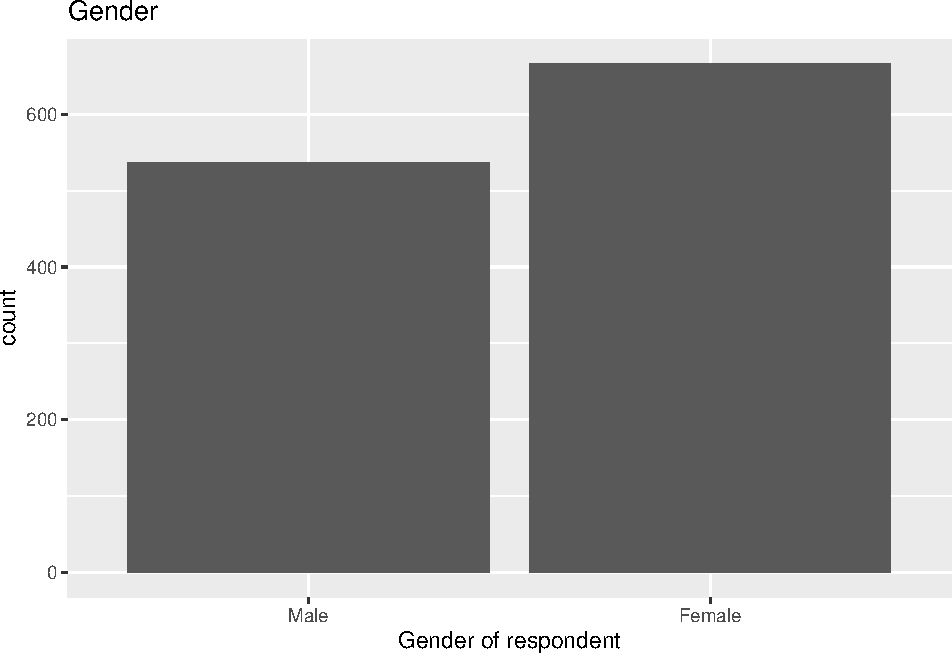
\includegraphics[width=1\linewidth]{lab-workbook_files/figure-latex/unnamed-chunk-65-1} \end{flushleft}

From the plot above, we can graphically see what we found out previously: there are more female respondents than males in our sample. The advantage is that we can have a sense of the magnitude of the difference by visualising it.

\hypertarget{bivariate-categorical-vs-categorical}{%
\subsection{Bivariate categorical vs categorical}\label{bivariate-categorical-vs-categorical}}

In Lab 3, we computed a Two-Way contingency table, which included the count of two categorical variables. This summary can be visualized using a stacked bar plot. This is quite similar to the above, with the addition that the area of the vertical plot is coloured by the size of each group.

If we wanted to know how gender is split by religion, we can add the \texttt{fill} argument with a second variable in aesthetics, as shown below.

\begin{Shaded}
\begin{Highlighting}[]
\FunctionTok{ggplot}\NormalTok{(nilt\_subset, }\FunctionTok{aes}\NormalTok{(}\AttributeTok{x =}\NormalTok{ rsex, }\AttributeTok{fill =}\NormalTok{ religcat)) }\SpecialCharTok{+}
  \FunctionTok{geom\_bar}\NormalTok{() }\SpecialCharTok{+}
  \FunctionTok{labs}\NormalTok{(}\AttributeTok{title =} \StringTok{\textquotesingle{}Gender by religion\textquotesingle{}}\NormalTok{, }\AttributeTok{x =} \StringTok{\textquotesingle{}Gender of respondent\textquotesingle{}}\NormalTok{)}
\end{Highlighting}
\end{Shaded}

\begin{flushleft}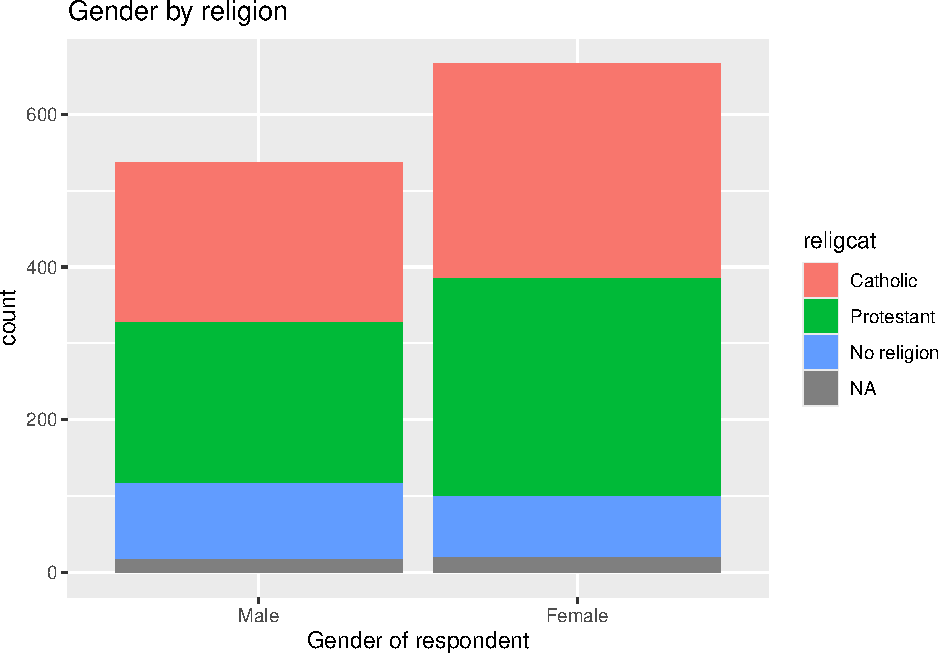
\includegraphics[width=1\linewidth]{lab-workbook_files/figure-latex/unnamed-chunk-66-1} \end{flushleft}

This plot is not very informative, since the total size of female and male respondents is different. The type of visualization will also depend on your specific research question or the topic you are interested in. For example, if I think it is worthwhile visualizing the religion by respondents' sex. A plot can show us the magnitudes and composition by respondents' sex for each religion. To do this, we need to change the aesthetics, specifying the religion by category variable \texttt{religcat} on the \texttt{x} axis and \texttt{fill} with gender \texttt{rsex}.

\begin{Shaded}
\begin{Highlighting}[]
\FunctionTok{ggplot}\NormalTok{(nilt\_subset, }\FunctionTok{aes}\NormalTok{(}\AttributeTok{x =}\NormalTok{ religcat, }\AttributeTok{fill =}\NormalTok{ rsex)) }\SpecialCharTok{+}
  \FunctionTok{geom\_bar}\NormalTok{() }\SpecialCharTok{+}
  \FunctionTok{labs}\NormalTok{(}\AttributeTok{title =} \StringTok{\textquotesingle{}Religion by gender\textquotesingle{}}\NormalTok{, }\AttributeTok{x =} \StringTok{\textquotesingle{}Religion\textquotesingle{}}\NormalTok{)}
\end{Highlighting}
\end{Shaded}

\begin{flushleft}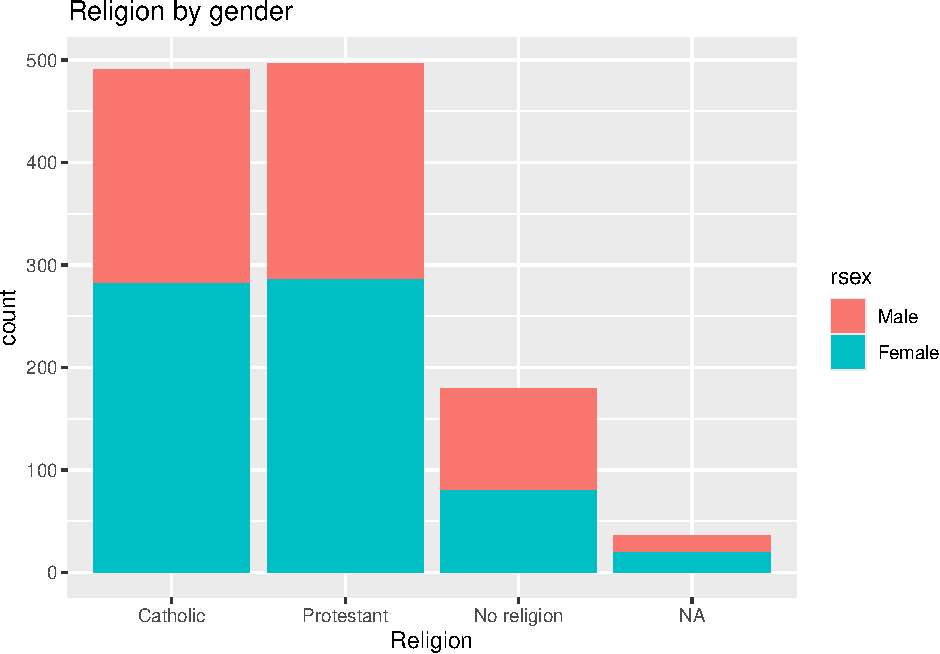
\includegraphics[width=1\linewidth]{lab-workbook_files/figure-latex/unnamed-chunk-67-1} \end{flushleft}

As we can see, catholic and protestant religion are equally popular among the respondents. Also, we can see that these are composed by similar proportions of males and females. One interesting thing is that there are more male respondents with no religion than female participants. Again, we found this out with the descriptive statistics computed in the last lab. However, we have the advantage that we can graphically reprsent and inspect the magnitude of these differences.

\hypertarget{numeric-variables}{%
\section{Numeric variables}\label{numeric-variables}}

\hypertarget{univariate-numeric}{%
\subsection{Univariate numeric}\label{univariate-numeric}}

Last time we talked about some measures of centrality and spread for numeric variables. The histogram plot is similar to the bar plot, the difference is that it splits the numeric range in fix ``bins'' and computes the frequency/count for each bin instead of counting the number of respondents for each numeric value. The syntax is practically the same as the simple bar plot. At this time, we set the the \texttt{x} aesthetic with the numeric variable age \texttt{rage}. Also, the geometry is defined as a histogram, using the \texttt{geom\_histogram()} function.

\begin{Shaded}
\begin{Highlighting}[]
\FunctionTok{ggplot}\NormalTok{(nilt\_subset, }\FunctionTok{aes}\NormalTok{(}\AttributeTok{x =}\NormalTok{ rage)) }\SpecialCharTok{+}
  \FunctionTok{geom\_histogram}\NormalTok{() }\SpecialCharTok{+}
  \FunctionTok{labs}\NormalTok{(}\AttributeTok{title =} \StringTok{\textquotesingle{}Age distribution\textquotesingle{}}\NormalTok{)}
\end{Highlighting}
\end{Shaded}

\begin{flushleft}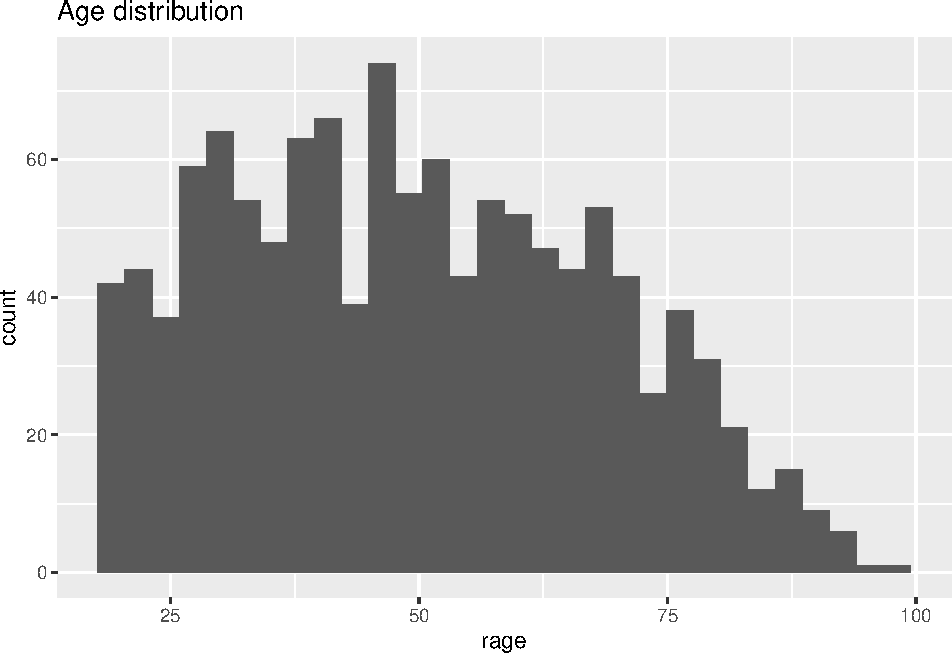
\includegraphics[width=1\linewidth]{lab-workbook_files/figure-latex/unnamed-chunk-68-1} \end{flushleft}

From the histogram, we have age (in bins) on the X axis, and the frequency/count on the y axis. This plot is useful to visualize how respondent's age is distributed in our sample. For instance, we can quickly see the minimum and maximum value, or the most popular age, or a general trend indicating the largest age group.

A second option to visualize numeric variables is the box plot. Essentially this draws the quartiles of a numeric vector. For this time, \texttt{rage} is defined in the \texttt{y} axis. This is just a personal preference. The geometry is set by the \texttt{geom\_boxplot()} function.

\begin{Shaded}
\begin{Highlighting}[]
\FunctionTok{ggplot}\NormalTok{(nilt\_subset, }\FunctionTok{aes}\NormalTok{(}\AttributeTok{y =}\NormalTok{ rage)) }\SpecialCharTok{+}
  \FunctionTok{geom\_boxplot}\NormalTok{() }\SpecialCharTok{+}
  \FunctionTok{labs}\NormalTok{(}\AttributeTok{title =} \StringTok{\textquotesingle{}Age boxplot\textquotesingle{}}\NormalTok{)}
\end{Highlighting}
\end{Shaded}

\begin{flushleft}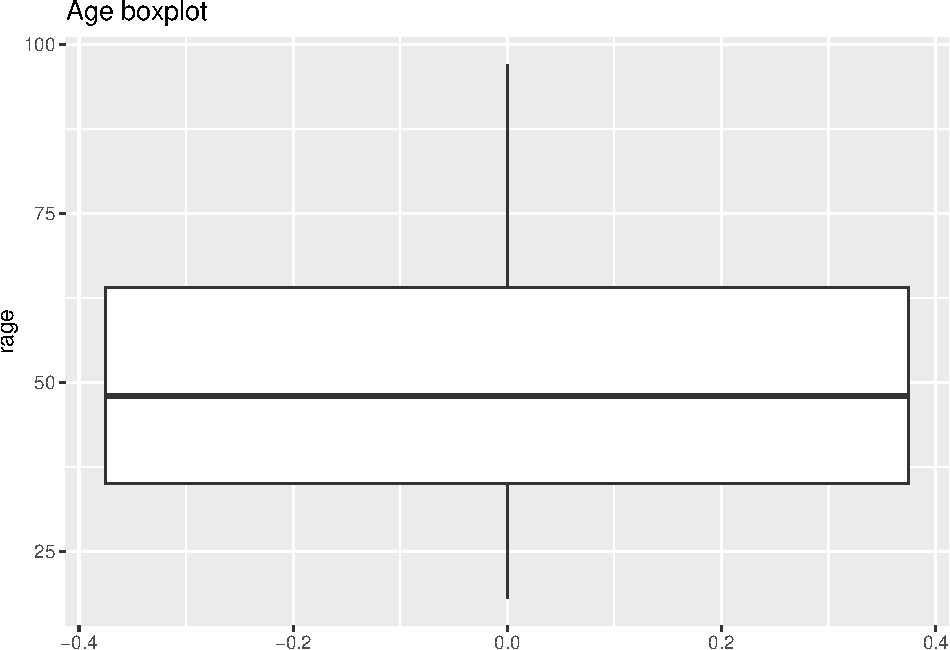
\includegraphics[width=1\linewidth]{lab-workbook_files/figure-latex/unnamed-chunk-69-1} \end{flushleft}

What we see from this plot is the first, second and third quartile. The second quartile (or median) is represented by the black line in the middle of the box. As you can see this is close to 50 years old, as we computed using the \texttt{quantile()} function. The lower edge of the box represents the 2nd quartile, which is somewhere around 35 years old. Similarly the 3rd quartile is represented by the upper edge of the box. We can confirm this by computing the quantiles for this variable.

\begin{Shaded}
\begin{Highlighting}[]
\FunctionTok{quantile}\NormalTok{(nilt\_subset}\SpecialCharTok{$}\NormalTok{rage, }\AttributeTok{na.rm =}\NormalTok{ T)}
\end{Highlighting}
\end{Shaded}

\begin{verbatim}
##   0%  25%  50%  75% 100% 
##   18   35   48   64   97
\end{verbatim}

\hypertarget{bivariate-numeric}{%
\subsection{Bivariate numeric}\label{bivariate-numeric}}

A useful plot to explore the relationship between two numeric variables is the scatter plot. This plot locates a dot for each observation according to to their respective numeric values. In the example below, we use age \texttt{rage} on the X axis (horizontal), and personal income \texttt{persinc2} on the Y axis (vertical). This type of plot is useful to explore a relationship between variables.

To generate a scatter plot, we need to define \texttt{x} and \texttt{y} in aesthetics \texttt{aes()}. The geometry is a point, expressed by \texttt{geom\_point()}. Note that we are specifying some further optional arguments. First, in \texttt{aes()} \texttt{alpha} regulates the opacity of the dots. This goes from 0.0 (completely translucent) to 1.0 (completely solid fill). Second, in \texttt{geom\_point()} we defined \texttt{position} as \texttt{jitter}. This arguments slightly moves the point away from their exact location. These two arguments are desired in this plot because the personal income bands are overlapped. Adding some transparency and \emph{noise} to their position, can allow to visualize possible patterns easily.

\begin{Shaded}
\begin{Highlighting}[]
\FunctionTok{ggplot}\NormalTok{(nilt\_subset, }\FunctionTok{aes}\NormalTok{(}\AttributeTok{x =}\NormalTok{ rage, }\AttributeTok{y =}\NormalTok{ persinc2, }\AttributeTok{alpha =} \FloatTok{0.8}\NormalTok{)) }\SpecialCharTok{+}
  \FunctionTok{geom\_point}\NormalTok{(}\AttributeTok{position =} \StringTok{"jitter"}\NormalTok{) }\SpecialCharTok{+}
  \FunctionTok{labs}\NormalTok{(}\AttributeTok{title =} \StringTok{\textquotesingle{}Personal income vs age\textquotesingle{}}\NormalTok{, }\AttributeTok{x =} \StringTok{\textquotesingle{}Age\textquotesingle{}}\NormalTok{, }\AttributeTok{y =} \StringTok{\textquotesingle{}Personal income (£)\textquotesingle{}}\NormalTok{)}
\end{Highlighting}
\end{Shaded}

\begin{flushleft}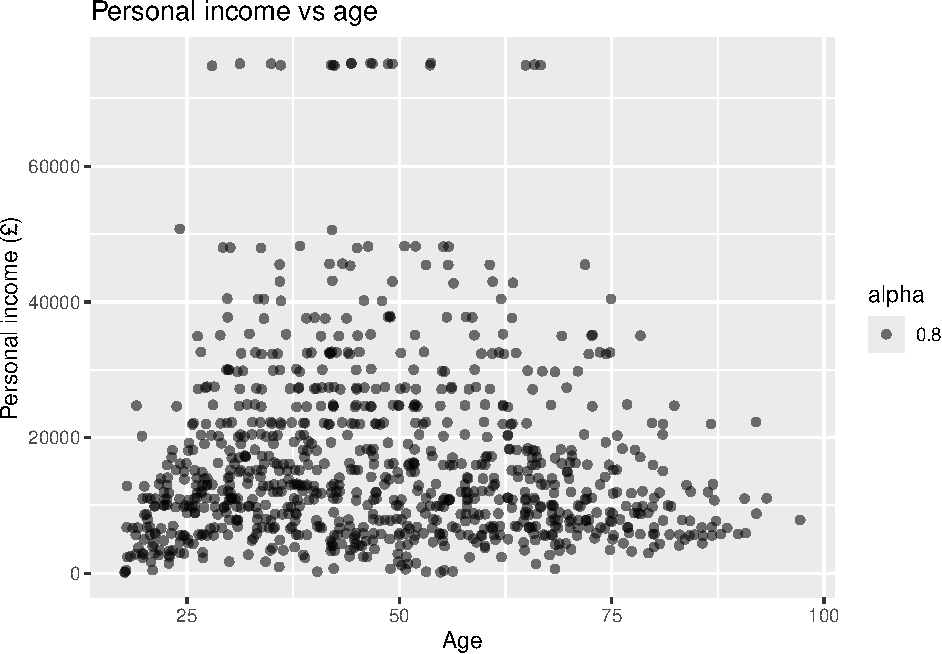
\includegraphics[width=1\linewidth]{lab-workbook_files/figure-latex/unnamed-chunk-71-1} \end{flushleft}

There is not a clear pattern in our previous plot. However, it is interesting to note that most of the people younger than 25 years old earn less than £20K a year. Similarly, most of the people older than 75 earn less than £20K. And only very few earn over £60k a year (looking at the top of the plot).

\hypertarget{mixed-data}{%
\section{Mixed data}\label{mixed-data}}

Very often we want to summarise central or spread measure by categories or groups. For example, let's go back to the example of age and respondents' sex. We can visualize these two variables (which include one numeric and one categorical) using a box plot. To create this, we need to specify the \texttt{x} and \texttt{y} value in \texttt{aes()} and include the \texttt{geom\_boxplot()} geometry.

\begin{Shaded}
\begin{Highlighting}[]
\FunctionTok{ggplot}\NormalTok{(nilt\_subset, }\FunctionTok{aes}\NormalTok{(}\AttributeTok{y =}\NormalTok{ rage, }\AttributeTok{x=}\NormalTok{ rsex)) }\SpecialCharTok{+}
  \FunctionTok{geom\_boxplot}\NormalTok{() }\SpecialCharTok{+}
  \FunctionTok{ggtitle}\NormalTok{(}\StringTok{\textquotesingle{}Age by sex\textquotesingle{}}\NormalTok{)}
\end{Highlighting}
\end{Shaded}

\begin{flushleft}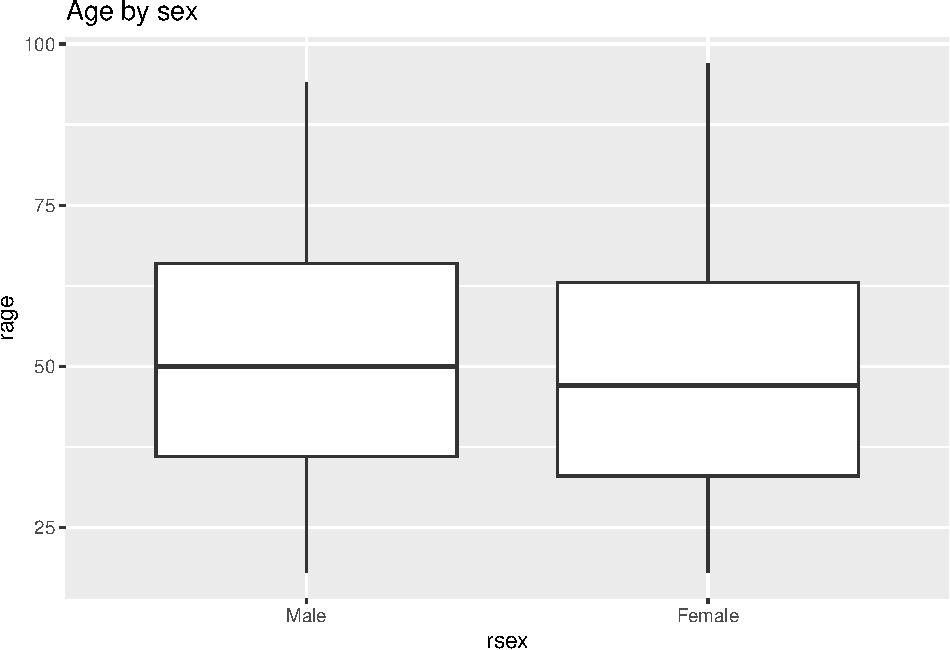
\includegraphics[width=1\linewidth]{lab-workbook_files/figure-latex/unnamed-chunk-72-1} \end{flushleft}

From this, we can visualize that female participants are slightly younger than their male counterparts in the sample.

\hypertarget{activity-6}{%
\section{Activity}\label{activity-6}}

Using the \texttt{nilt\_subset} object, complete the tasks below in the Rmd file \texttt{Lab\_6}, which you created earlier. Insert a new code chunk for each of these activities and include brief comments as text (outside the chunk) in the Rmd document to introduce or describe the plots. Feel free to copy and adapt the code to create the plots in the examples above.

\begin{itemize}
\tightlist
\item
  Create a first-level header to start a section called ``Categorical analysis'';
\item
  Create simple bar plot using the \texttt{geom\_bar()} geometry to visualize the political affiliation reported by the respondents using the variable \texttt{uninatid};
\item
  Based on the plot above, create a `stacked bar plot' to visualize the political affiliation by religion, using the \texttt{uninatid} and \texttt{religcat} variables;
\item
  Create a new first-level header to start a section called ``Numeric analysis'';
\item
  Create a scatter plot about the relationship between personal income \texttt{persinc2} on the Y axis and number of hours worked a week \texttt{rhourswk} on the X axis;
\item
  Finally, create a box plot to visualize personal income \texttt{persinc2} on the Y axis and self-reported level of happiness \texttt{ruhappy} on the x axis\ldots{} Interesting result, Isn't it? Talk to your lab group-mates and tutors about your results on Zoom (live) or your Lab Group on Teams (online anytime);
\item
  Add your own (brief) comments to each of the plots as text in your Rmd file;
\item
  Knit the .Rmd document as HTML or PDF. The knitted file will be saved automatically in your project. You can come back to the Rmd file to make changes if needed and knit it again as many times as you wish.
\end{itemize}

\hypertarget{r-cheatsheets}{%
\subsection{R Cheatsheets}\label{r-cheatsheets}}

There are a number of features that you can customize in your plots, including the background, text size, colours, adding more variables. But you don't have to memorise or remember all this, one thing that is very commonly used by R data scientists are R cheat sheets! They are extremely handy when you try to create a visualisation from scratch, check out the \href{https://rstudio.com/wp-content/uploads/2015/03/ggplot2-cheatsheet.pdf}{Data Visualization with ggplot2 Cheat Sheet}. An extra tip is that you can change the overall look of the plot by adding pre-defined themes. You can read more about it \href{https://ggplot2.tidyverse.org/reference/ggtheme.html}{here}. Another interesting site is the \href{https://www.r-graph-gallery.com/}{The R Graph Gallery}, which includes a comprehensive showcase of plot types and their respective code.

\hypertarget{correlation}{%
\chapter{Correlation}\label{correlation}}

\hypertarget{what-is-correlation}{%
\section{What is correlation?}\label{what-is-correlation}}

When conducting empirical research, we are often interested in associations between two variables, for example, personal income and attitudes towards migrants. In this lab we will focus on visualizing relationship between variables and how to measure it. In quantitative research, the main variable of interest in an analysis is called the \emph{dependent} or \emph{response variable}, and the second is known as the \emph{independent} or \emph{explanatory}. In the example above, we can think of personal income as the independent variable and attitudes as the dependent.

The relationship between variables can be positive, negative or non-existent. The figure below shows these type of relationships to different extents. The association is positive when one of the variables increases and the second variable tends to go in the same direction (that is increasing as well). The first plot on the left-hand side shows a strong positive relationship. As you can see, the points are closely clustered around the straight line. The next plot also shows a positive relationship. This time the relationship is moderate. Therefore, the points are more dispersed in relation to the line compared to the previous one.

\begin{figure}

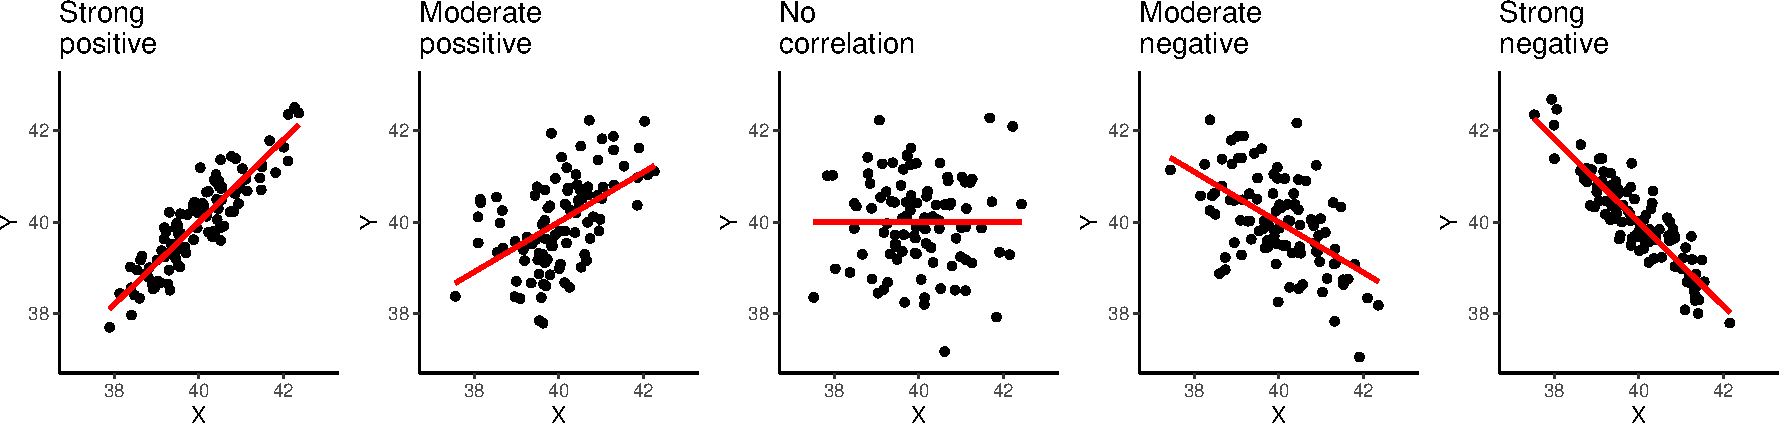
\includegraphics[width=1\linewidth]{lab-workbook_files/figure-latex/unnamed-chunk-73-1} \hfill{}

\caption{\label{fig:figs} Types of correlation.}\label{fig:unnamed-chunk-73}
\end{figure}

The plot in the middle, shows two variables that are not correlated. The location of the points is not following any pattern and the line is flat. By contrast, the last two plots on the right hand-side show a negative relationship. When the values on the X axis increase, the values on the Y axis tend to decrease.

\hypertarget{data-and-r-environment}{%
\subsection{Data and R environment}\label{data-and-r-environment}}

We will continue working on the same R Studio Cloud project as in the previous session and using the 2012 \href{https://www.ark.ac.uk/nilt/}{Northern Ireland Life and Times Survey (NILT)} data. To set the \texttt{R} environment please follow the next steps:

\begin{enumerate}
\def\labelenumi{\arabic{enumi}.}
\tightlist
\item
  Please go to your `Quants lab group' in \href{https://rstudio.cloud/}{RStudio Cloud} (log in if necessary);
\item
  Open your own copy of the `NILT' project from the `Quants lab group';
\item
  Create a new Rmd file, type `Correlation analysis' in `Tile' section and your name in the `Author' box. Leave the `Default Output Format' as \texttt{HTML}.
\item
  Save the Rmd document under the name `Lab7\_correlation'.
\item
  Delete all the contents in the Rmd default example with the exception of the first bit which contains the YAML and the first chunk, which contains the default chunk options (that is all from line 12 and on).
\item
  In the setup chunk, change \texttt{echo} from \texttt{TRUE} to \texttt{FALSE} in line 9 (this will hide the code for all chunks in your final document).
\item
  Within the first chunk, copy and paste the following code below line 9 \texttt{knitr::opts\_chunk\$set(message\ =\ FALSE,\ warning\ =\ FALSE)}. This will hide the warnings and messages when you load the packages.
\end{enumerate}

In the Rmd document insert a new a chunk, copy and paste the following code. Then, run the individual chunk by clicking on the green arrow on the top-right of the chunk.

\begin{Shaded}
\begin{Highlighting}[]
\DocumentationTok{\#\# Load the packages}
\FunctionTok{library}\NormalTok{(tidyverse)}
\CommentTok{\# Load the data from the .rds file we created in lab 3}
\NormalTok{nilt }\OtherTok{\textless{}{-}} \FunctionTok{readRDS}\NormalTok{(}\StringTok{"data/nilt\_r\_object.rds"}\NormalTok{)}
\end{Highlighting}
\end{Shaded}

This time we will use new variables from the survey. Therefore, we need to coerce them into their appropriate type first. Insert a second chunk, copy and paste the code below. Then, run the individual chunk.

\begin{Shaded}
\begin{Highlighting}[]
\CommentTok{\# Age of respondent’s spouse/partner}
\NormalTok{nilt}\SpecialCharTok{$}\NormalTok{spage }\OtherTok{\textless{}{-}} \FunctionTok{as.numeric}\NormalTok{(nilt}\SpecialCharTok{$}\NormalTok{spage)}
\CommentTok{\# Migration}
\NormalTok{nilt }\OtherTok{\textless{}{-}} \FunctionTok{mutate\_at}\NormalTok{(nilt, }\FunctionTok{vars}\NormalTok{(mil10yrs, miecono, micultur), as.numeric)}
\end{Highlighting}
\end{Shaded}

Also, we will create a new variable called \texttt{mig\_per} by summing the respondent's opinion in relation to migration using the following variables: \texttt{mil10yrs}, \texttt{miecono} and \texttt{micultur} (see the documentation p.~14 \href{https://www.ark.ac.uk/teaching/NILT2012TeachingResources.pdf}{here} to know more about these variables). Again, insert a new chunk, copy and paste the code below, and run the individual chunk.

\begin{Shaded}
\begin{Highlighting}[]
\CommentTok{\# overall perception towards migrants}
\NormalTok{nilt }\OtherTok{\textless{}{-}} \FunctionTok{rowwise}\NormalTok{(nilt) }\SpecialCharTok{\%\textgreater{}\%} 
  \CommentTok{\# sum values}
  \FunctionTok{mutate}\NormalTok{(}\AttributeTok{mig\_per =} \FunctionTok{sum}\NormalTok{(mil10yrs, miecono, micultur, }\AttributeTok{na.rm =}\NormalTok{ T )) }\SpecialCharTok{\%\textgreater{}\%} 
  \FunctionTok{ungroup}\NormalTok{() }\SpecialCharTok{\%\textgreater{}\%} 
  \CommentTok{\# assign NA to values that sum 0}
  \FunctionTok{mutate}\NormalTok{(}\AttributeTok{mig\_per =}  \FunctionTok{na\_if}\NormalTok{(mig\_per, }\DecValTok{0}\NormalTok{))}
\end{Highlighting}
\end{Shaded}

\hypertarget{visualizing-correlation}{%
\subsection{Visualizing correlation}\label{visualizing-correlation}}

Visualizing two or more variables can help to uncover or understand the relationship between these variables. As briefly introduced in the previous session, different types of plots are appropriate for different types of variables. Therefore, we split the following sections according to the type of data to be analysed.

You do not need to run or reproduce the examples shown in the following sections in your R session with the exception of exercises that are under the \emph{activity} headers.

\hypertarget{numeric-vs-numeric}{%
\subsubsection{Numeric vs numeric}\label{numeric-vs-numeric}}

To illustrate this type of correlation, let's start with a relatively obvious but useful example. Suppose we are interested in how people choose their spouse or partner. The first characteristic that we might look at is age. We might suspect that there is a correlation between the the \texttt{nilt} respondents' won age and their partner's age. Since both ages are numeric variables, a scatter plot is appropriate to visualize the correlation. To do this, let's use the functions \texttt{ggplot()} and \texttt{geom\_point()}. In aesthetics \texttt{aes()} let's define the respondent's age \texttt{rage} in the X axis and the respondent's spouse/partner age \texttt{spage} in the Y axis. As a general convention in quantitative research, the response/dependent variable is visualized on the Y axis and the independent on the X axis (you do not need to copy and reproduce the example below).

\begin{Shaded}
\begin{Highlighting}[]
\FunctionTok{ggplot}\NormalTok{(nilt, }\FunctionTok{aes}\NormalTok{(}\AttributeTok{x =}\NormalTok{ rage, }\AttributeTok{y =}\NormalTok{ spage)) }\SpecialCharTok{+} 
  \FunctionTok{geom\_point}\NormalTok{() }\SpecialCharTok{+}
  \FunctionTok{geom\_smooth}\NormalTok{(}\AttributeTok{method =} \StringTok{"lm"}\NormalTok{, }\AttributeTok{se =} \ConstantTok{FALSE}\NormalTok{) }\SpecialCharTok{+}
  \FunctionTok{labs}\NormalTok{(}\AttributeTok{title =} \StringTok{"Respondent\textquotesingle{}s age vs respondent’s spouse/partner age"}\NormalTok{, }
       \AttributeTok{x =} \StringTok{"Respondent\textquotesingle{}s age"}\NormalTok{, }\AttributeTok{y =} \StringTok{"Respondent’s spouse/partner age"}\NormalTok{ )}
\end{Highlighting}
\end{Shaded}

\begin{flushleft}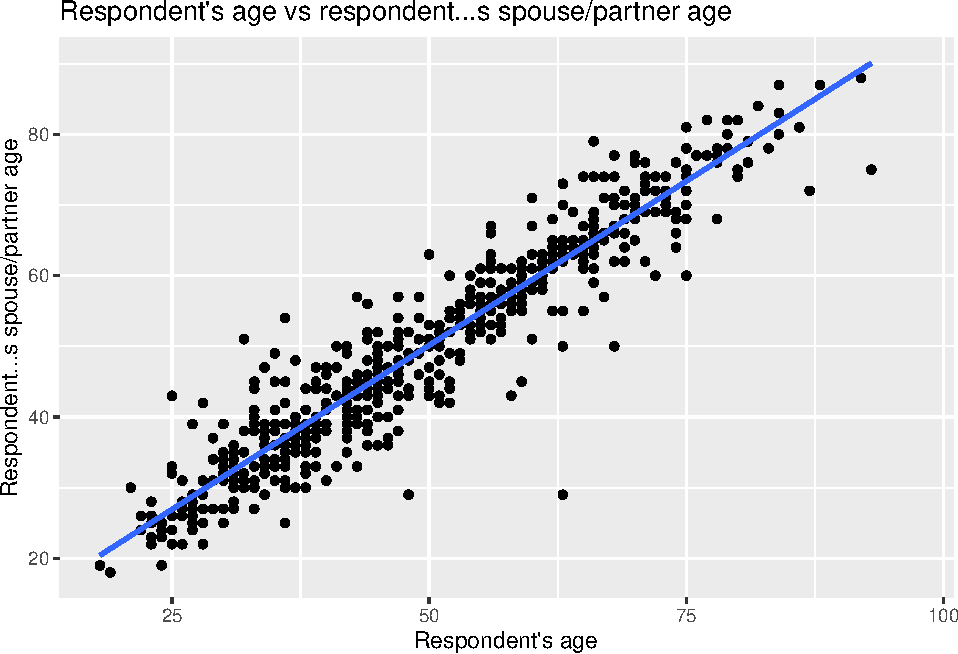
\includegraphics[width=1\linewidth]{lab-workbook_files/figure-latex/unnamed-chunk-77-1} \end{flushleft}

Note that in this plot the function \texttt{geom\_smooth()} was used. This is to plot a straight line which describes the best all the points in the graph.

From the plot above, we see that there is a strong positive correlation between the respondent's age and their partner's age. We see that for some individuals their partner's age is older, whereas others is younger. Also, there are some dots that are far away from the straight line. For example, in one case the respondent is around 60 years old and the age of their partner is around 30 years old (can you find that dot on the plot?). These extreme values are known as \emph{outliers}.

We may also suspect that the respondents' sex is playing a role in this relationship. We can include this as a third variable in the plot by colouring the dots by the respondents' sex. To do this, let's specify the \texttt{colour} argument in aesthetics \texttt{aes()} with a categorical variable \texttt{rsex}.

\begin{Shaded}
\begin{Highlighting}[]
\FunctionTok{ggplot}\NormalTok{(nilt, }\FunctionTok{aes}\NormalTok{(}\AttributeTok{x =}\NormalTok{ rage, }\AttributeTok{y =}\NormalTok{ spage, }\AttributeTok{colour =}\NormalTok{ rsex)) }\SpecialCharTok{+} 
  \FunctionTok{geom\_point}\NormalTok{() }\SpecialCharTok{+}
  \FunctionTok{geom\_abline}\NormalTok{(}\AttributeTok{slope =} \DecValTok{1}\NormalTok{, }\AttributeTok{intercept =} \DecValTok{0}\NormalTok{, }\AttributeTok{colour =} \StringTok{"gray20"}\NormalTok{) }\SpecialCharTok{+}
  \FunctionTok{labs}\NormalTok{(}\AttributeTok{title =} \StringTok{"Respondent\textquotesingle{}s age vs respondent’s spouse/partner age"}\NormalTok{, }
       \AttributeTok{x =} \StringTok{"Respondent\textquotesingle{}s age"}\NormalTok{, }\AttributeTok{y =} \StringTok{"Respondent’s spouse/partner age"}\NormalTok{ )}
\end{Highlighting}
\end{Shaded}

\begin{flushleft}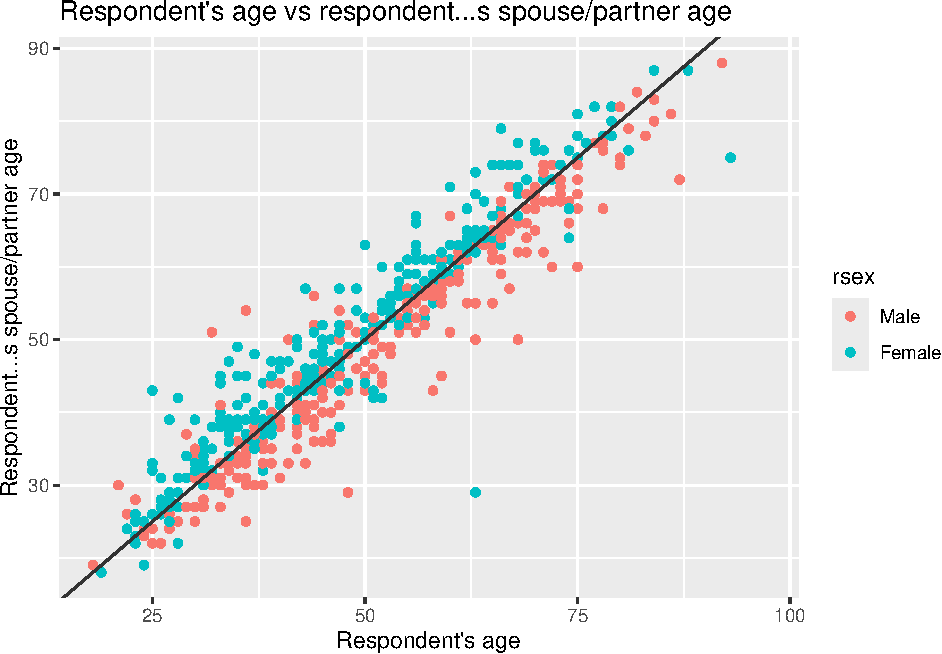
\includegraphics[width=1\linewidth]{lab-workbook_files/figure-latex/unnamed-chunk-78-1} \end{flushleft}

In the previous plot, we included a line which describes what it would look like if the partner's age were exactly the same as the respondent's age. We observe a clear pattern in which female participants are on one side of the line and males on the other. As we can see, most female respondents tend to choose/have partners who are older, whereas males younger ones.

\hypertarget{activity-1-2}{%
\subsection{Activity 1}\label{activity-1-2}}

In the \texttt{Lab7\_correlation} file, use the \texttt{nilt} data object to visualize the relationship of the following variables by creating a new chunk. Run the chunk individually and comment on what you observe from the result as text (outside the code chunks).

\begin{itemize}
\tightlist
\item
  Create a scatter plot to visualize the correlation between the respondent's overall opinion in relation to migration \texttt{mig\_per} and the respondent's age \texttt{rage}. Remember that we just created the \texttt{mig\_per} variable by summing three variables which were in a 0-10 scale (the higher the value, the better the person's perception is). In \texttt{aes()}, specify \texttt{rage} on the X axis and \texttt{mig\_per} on the Y axis. Use \texttt{ggplot()} function and \texttt{geom\_point()}. Also, include a straight line describing the points using the \texttt{geom\_smooth()} function. Within this function set the \texttt{method} argument to \texttt{\textquotesingle{}lm\textquotesingle{}}.
\item
  What type of relationship do you observe? Comment as text in the Rmd the overall result of the plot and whether this is in line with your previous expectation.
\end{itemize}

\hypertarget{numeric-vs-categorical}{%
\subsubsection{Numeric vs categorical}\label{numeric-vs-categorical}}

As briefly introduced in the last lab, correlations often occur between categorical and numeric data. A good way to observe the relationship between these type of variables is using a box plot. Which essentially shows the distribution of the numeric values by category/group.

Let's say we are interested in the relationship between education level and perception of migration. The variable \texttt{highqual} contains the respondent's highest education qualification. Using \texttt{ggplot()}, we can situate \texttt{mig\_per} on the X axis and \texttt{highqual} on the Y axis, and plot it with the \texttt{gem\_boxplot()} function. Note that before passing the dataset to \texttt{ggplot}, we can filter out two categories of the variable \texttt{highqual} where education level is unknown (i.e.~``Other, level unknown'' or ``Unclassified'').

\begin{Shaded}
\begin{Highlighting}[]
\NormalTok{nilt }\SpecialCharTok{\%\textgreater{}\%} 
  \FunctionTok{filter}\NormalTok{(highqual }\SpecialCharTok{!=} \StringTok{"Other, level unknown"} \SpecialCharTok{\&}\NormalTok{ highqual }\SpecialCharTok{!=} \StringTok{"Unclassified"}\NormalTok{) }\SpecialCharTok{\%\textgreater{}\%} 
  \FunctionTok{ggplot}\NormalTok{(}\FunctionTok{aes}\NormalTok{(}\AttributeTok{x =}\NormalTok{ mig\_per, }\AttributeTok{y =}\NormalTok{ highqual )) }\SpecialCharTok{+}
  \FunctionTok{geom\_boxplot}\NormalTok{()}
\end{Highlighting}
\end{Shaded}

\begin{flushleft}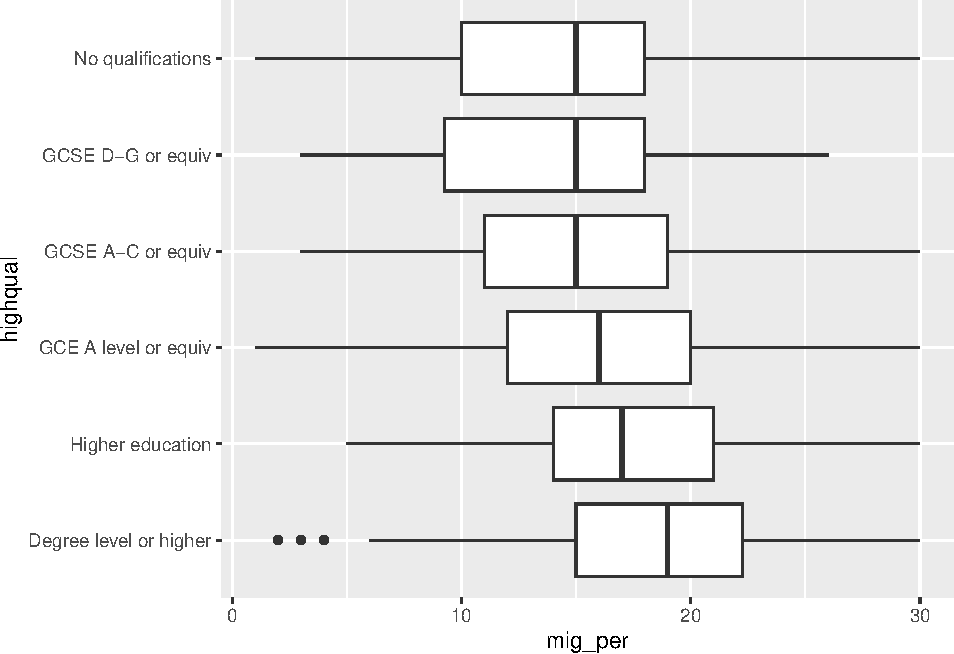
\includegraphics[width=1\linewidth]{lab-workbook_files/figure-latex/unnamed-chunk-79-1} \end{flushleft}

From the plot above, we see that respondents with higher education level (on the bottom) appear to have more positive opinion on migration when compared to respondents with lower education level or no qualifications (on the top). Overall, the data shows a pattern that the lower one's education level is, the worse their opinion towards migration is likely to be. Since education level is an ordinal variable, we can say this is a positive relationship.

\hypertarget{activity-2-2}{%
\subsection{Activity 2}\label{activity-2-2}}

Using the \texttt{nilt} data object, visualize the relationship of the following variables by creating a new chunk. Run the chunk individually and comment on what you can observe from the results as text in the Rmd file to introduce the plot.

\begin{itemize}
\tightlist
\item
  Create a boxplot to visualize the correlation between the respondent's overall opinion in relation to migration \texttt{mig\_per} and the political party which the respondent identify with \texttt{uninatid}. Use \texttt{ggplot()} in combination with \texttt{geom\_boxplot()}. Make sure to specify \texttt{mig\_per} on the Y axis and \texttt{uninatid} on the X axis in \texttt{aes()}.
\item
  Do you think the opinion towards migration differs among the groups in the plot? Comment on the overall results in the Rmd document.
\end{itemize}

\hypertarget{measuring-correlation}{%
\section{Measuring correlation}\label{measuring-correlation}}

So far we have examined correlation by visualizing variables only. A useful practice in quantitative research is to actually measure the magnitude of the relationship between these variables. One common measure is the \emph{Pearson} correlation coefficient. This measure results in a number that goes from -1 to 1. A coefficient below 0 implies a negative correlation whereas a coefficient over 0 a positive one. When the coefficient is close to positive one (1) or negative one (-1), it implies that the relationship is strong. By contrast, coefficients close to 0 indicate a weak relationship. This technique is appropriate to measure linear numeric relationships, which is when we have numeric variables with a normal distribution, e.g.~age in our dataset.

Let's start measuring the relationship between the respondent's age and their partner's age. To do this in R, we should use the \texttt{cor()} function. In the R syntax, first we specify the variables separated by a comma. We need to be explicit by specifying the object name, the dollar sign, and the name of the variable, as shown below. Also, I set the \texttt{use} argument as \texttt{\textquotesingle{}pairwise.complete.obs\textquotesingle{}}. This is because one or both of the variables contain more than one missing value. Therefore, we are telling R to use complete observations only.

\begin{Shaded}
\begin{Highlighting}[]
\FunctionTok{cor}\NormalTok{(nilt}\SpecialCharTok{$}\NormalTok{rage, nilt}\SpecialCharTok{$}\NormalTok{spage, }\AttributeTok{use =} \StringTok{\textquotesingle{}pairwise.complete.obs\textquotesingle{}}\NormalTok{)}
\end{Highlighting}
\end{Shaded}

\begin{verbatim}
## [1] 0.9481297
\end{verbatim}

The correlation coefficient between this variables is 0.95. This is close to positive 1. Therefore, it is a strong positive correlation. The result is completely in line with the plot above, since we saw how the dots were close to the straight line.

What about the relationship between \texttt{age} and \texttt{mig\_per} that you plotted earlier?

\begin{Shaded}
\begin{Highlighting}[]
\FunctionTok{cor}\NormalTok{(nilt}\SpecialCharTok{$}\NormalTok{rage, nilt}\SpecialCharTok{$}\NormalTok{mig\_per, }\AttributeTok{use =} \StringTok{\textquotesingle{}pairwise.complete.obs\textquotesingle{}}\NormalTok{)}
\end{Highlighting}
\end{Shaded}

\begin{verbatim}
## [1] -0.05680918
\end{verbatim}

The coefficient is very close to 0, which means that the correlation is practically non-existent. The absence of correlation is also interesting in research. For instance, one might expect that younger people would be more open to migration. However, it seems that age does not play a role on people's opinion about migration in NI according to this data.

Let's say that we are interested in the correlation between \texttt{mig\_per} and all other numeric variables in the dataset. Instead of continuing computing the correlation one by one, we can run a correlation matrix. The code syntax can be read as follows: from the \texttt{nilt} data select these variables, then compute the correlation coefficient using complete cases, and then round the result to 3 decimals.

\begin{Shaded}
\begin{Highlighting}[]
\NormalTok{nilt }\SpecialCharTok{\%\textgreater{}\%} 
  \FunctionTok{select}\NormalTok{(mig\_per, rage, spage, rhourswk, persinc2) }\SpecialCharTok{\%\textgreater{}\%} 
  \FunctionTok{cor}\NormalTok{(}\AttributeTok{use =} \StringTok{\textquotesingle{}pairwise.complete.obs\textquotesingle{}}\NormalTok{) }\SpecialCharTok{\%\textgreater{}\%} 
  \FunctionTok{round}\NormalTok{(}\DecValTok{3}\NormalTok{)}
\end{Highlighting}
\end{Shaded}

\begin{verbatim}
##          mig_per   rage  spage rhourswk persinc2
## mig_per    1.000 -0.057 -0.132    0.082    0.228
## rage      -0.057  1.000  0.948   -0.013   -0.036
## spage     -0.132  0.948  1.000   -0.182   -0.090
## rhourswk   0.082 -0.013 -0.182    1.000    0.383
## persinc2   0.228 -0.036 -0.090    0.383    1.000
\end{verbatim}

From the result above, we have a correlation matrix that computes the \emph{Person} correlation coefficient for the selected variables. In the first row we have migration perception. You will notice that the first value is 1.00, this is because it is measuring the correlation against the same variable (i.e.~itself). The next value in the first row is age, which is nearly 0. The next variables also result in low coefficients, with the exception of the personal income, where we see a moderate/low positive correlation. This can be interpreted that respondents with high income are associated with more positive opinion towards migration compared to low-income respondents.

\hypertarget{activity-3-1}{%
\subsection{Activity 3}\label{activity-3-1}}

\begin{itemize}
\tightlist
\item
  Insert a new chunk in your Rmd file;
\item
  Using the \texttt{nilt} data object, compute a correlation matrix using the following variables: \texttt{rage}, \texttt{persinc2}, \texttt{mil10yrs}, \texttt{miecono} and \texttt{micultur}, setting the \texttt{use} argument to \texttt{\textquotesingle{}pairwise.complete.obs\textquotesingle{}} and rounding the result to 3 decimals;
\item
  Run the chunk individually and comment whether personal income or age is correlated with the perception of migrants in relation to the specific aspects asked in the variables measured (consult the documentation in p.~14 to get a description of these variables);
\item
  Knit the \texttt{Lab7\_correlation} Rmd document to \texttt{.html} or \texttt{.pdf}. The output document will automatically be saved in your project.
\item
  Discuss your previous results with your neighbour or tutor.
\end{itemize}

\hypertarget{simple-lm}{%
\chapter{Linear model: Simple linear regression}\label{simple-lm}}

\hypertarget{welcome}{%
\section{Welcome}\label{welcome}}

In the previous lab we learned about correlation. We visualised the relationship of different types of variables. Also, we computed one correlation measure for two numeric variables, \emph{Pearson} correlation. This measure is useful to compute the strength and the direction of the association. However, it presents some limitations, e.g.~it can only be used for numeric variables, it allows only one variable at a time, and it is appropriate to describe a linear relationship.

Linear regression can overcome some of these limitations and it can be extended to achieve further purposes (e.g.~use multiple variables or estimate scenarios). This technique is in fact very common and one of the most popular in quantitative research in social sciences. Therefore, getting familiar with it will be important for you not only to perform your own analyses, but also to interpret and critically read literature.

\hypertarget{introduction-to-simple-linear-regression}{%
\section{Introduction to simple linear regression}\label{introduction-to-simple-linear-regression}}

IMPORTANT: Linear regression is appropriate only when the dependent variable is \textbf{numeric} (interval/ratio).

However, the independent variables can be categorical, ordinal, or numeric. Also, you can include more than one independent variable to evaluate how these relate to the dependent variable. In this lab we will start using only one explanatory variable. This is know as simple linear regression.

\hypertarget{the-idea-behind}{%
\subsection{The idea behind}\label{the-idea-behind}}

For this lab, we will continue using the 2012 NILT survey to introduce linear models. To do so, please set your RStudio environment as follows:

\begin{enumerate}
\def\labelenumi{\arabic{enumi}.}
\tightlist
\item
  Go to your `Quants lab group' in \href{https://rstudio.cloud/}{RStudio Cloud};
\item
  Create a copy of the project called `NILT2' which is located in your `Quants lab group' by clicking on the `Start' button;
\item
  Once in the project, create a new `R Script' file (a simple \texttt{R} script NOT an .Rmd file);
\item
  Save the \texttt{R} file as `linear\_model\_intro'.
\end{enumerate}

Reproduce the code below, by copying, pasting and running it from your new script and focus on the intuitive part of this section.

First, load the \texttt{tidyverse} library and read the \texttt{nilt\_r\_object.rds} file which is stored in the folder called `data' and contains the NILT survey (\texttt{tidyverse} was installed in your session already).

\begin{Shaded}
\begin{Highlighting}[]
\DocumentationTok{\#\# Load the packages}
\FunctionTok{library}\NormalTok{(tidyverse)}
\CommentTok{\# Read the data from the .rds file}
\NormalTok{nilt }\OtherTok{\textless{}{-}} \FunctionTok{readRDS}\NormalTok{(}\StringTok{"data/nilt\_r\_object.rds"}\NormalTok{)}
\end{Highlighting}
\end{Shaded}

This dataset is exactly the same as the one you processed in previous labs.

We will re-revisit the example of the respondent's spouse/partner characteristics. To keep things simple, let's create a minimal sample of the dataset including only 40 random observations:

\begin{Shaded}
\begin{Highlighting}[]
\CommentTok{\# select a small random sample}
\FunctionTok{set.seed}\NormalTok{(}\DecValTok{3}\NormalTok{)}
\CommentTok{\# Filter where partner\textquotesingle{}s age is not NA and take a random sample of 40}
\NormalTok{nilt\_sample }\OtherTok{\textless{}{-}} \FunctionTok{filter}\NormalTok{(nilt, }\SpecialCharTok{!}\FunctionTok{is.na}\NormalTok{(spage)) }\SpecialCharTok{\%\textgreater{}\%} \FunctionTok{sample\_n}\NormalTok{(}\DecValTok{40}\NormalTok{)}
\CommentTok{\# Select only respondent\textquotesingle{}s age and spouse/partner\textquotesingle{}s age}
\NormalTok{nilt\_sample }\OtherTok{\textless{}{-}} \FunctionTok{select}\NormalTok{(nilt\_sample, rage, spage)}
\end{Highlighting}
\end{Shaded}

We will start by creating a scatter plot using the respondent's spouse/partner age \texttt{spage} on the Y axis, and the respondent's \texttt{rage} on the X axis.

\begin{Shaded}
\begin{Highlighting}[]
\CommentTok{\# plot}
\FunctionTok{ggplot}\NormalTok{(nilt\_sample,  }\FunctionTok{aes}\NormalTok{(}\AttributeTok{x =}\NormalTok{ rage, }\AttributeTok{y =}\NormalTok{ spage)) }\SpecialCharTok{+} 
  \FunctionTok{geom\_point}\NormalTok{(}\AttributeTok{position =} \StringTok{"jitter"}\NormalTok{) }\SpecialCharTok{+}
  \FunctionTok{labs}\NormalTok{(}\AttributeTok{title =} \StringTok{"Respondent\textquotesingle{}s age vs respondent’s spouse/partner age"}\NormalTok{, }
       \AttributeTok{x =} \StringTok{"Respondent\textquotesingle{}s age"}\NormalTok{, }\AttributeTok{y =} \StringTok{"Respondent’s spouse/partner age"}\NormalTok{ )}
\end{Highlighting}
\end{Shaded}

\begin{flushleft}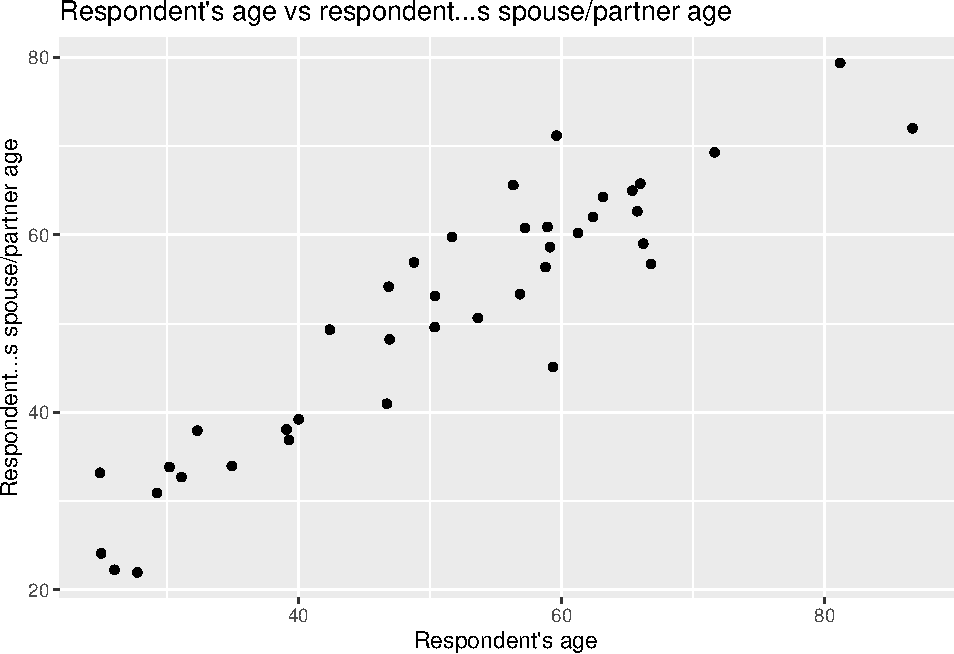
\includegraphics[width=1\linewidth]{lab-workbook_files/figure-latex/unnamed-chunk-85-1} \end{flushleft}

As you can see, even with this minimal example using 40 observations, there is a clear trend. From the plot, it seems intuitive to draw a line that describes this general trend. Imagine a friend will draw this line for you. You will have to tell them some basic references on how to do it. You can, for example, specify a start point and and end point in the plot. Alternatively, which is what we will do below, you can specify a start point and a value that describes the slope of the line. For now, our friend is \texttt{ggplot}. You have to pass these two values (start point and slope) in the \texttt{geom\_abline()} function to draw a line which describes these points.

\begin{Shaded}
\begin{Highlighting}[]
\FunctionTok{ggplot}\NormalTok{(nilt\_sample, }\FunctionTok{aes}\NormalTok{(}\AttributeTok{x =}\NormalTok{ rage, }\AttributeTok{y =}\NormalTok{ spage)) }\SpecialCharTok{+} 
  \FunctionTok{geom\_point}\NormalTok{() }\SpecialCharTok{+}
  \FunctionTok{geom\_abline}\NormalTok{(}\AttributeTok{slope =} \DecValTok{1}\NormalTok{, }\AttributeTok{intercept =} \DecValTok{0}\NormalTok{, }\AttributeTok{colour =} \StringTok{"red"}\NormalTok{) }\SpecialCharTok{+}
  \FunctionTok{labs}\NormalTok{(}\AttributeTok{title =} \StringTok{"Respondent\textquotesingle{}s age vs respondent’s spouse/partner age"}\NormalTok{, }
       \AttributeTok{x =} \StringTok{"Respondent\textquotesingle{}s age"}\NormalTok{, }\AttributeTok{y =} \StringTok{"Respondent’s spouse/partner age"}\NormalTok{ )}
\end{Highlighting}
\end{Shaded}

\begin{flushleft}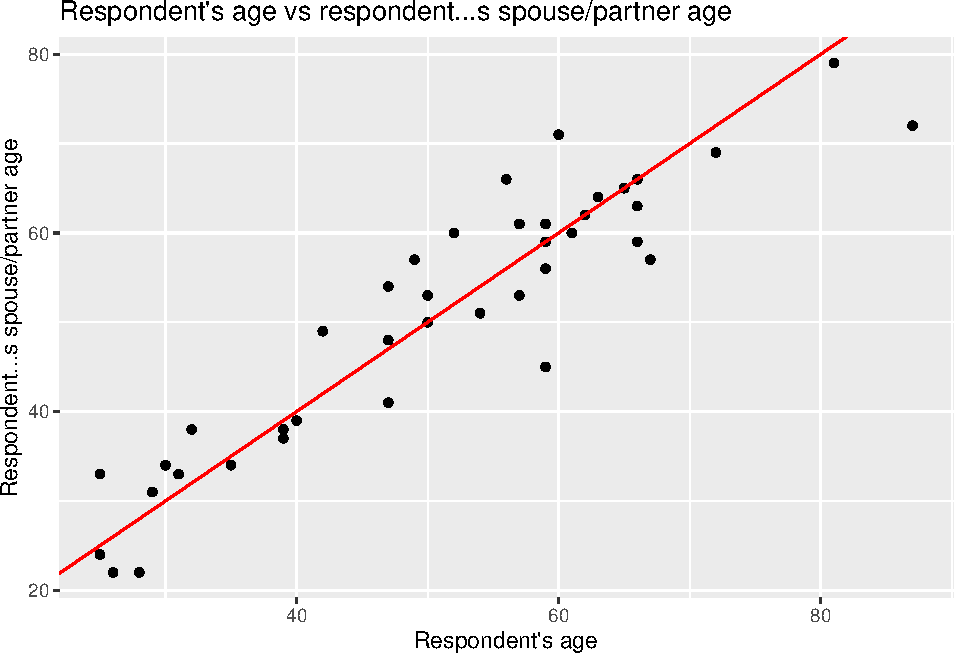
\includegraphics[width=1\linewidth]{lab-workbook_files/figure-latex/unnamed-chunk-86-1} \end{flushleft}

In the guess above, it is assumed that the age of the spouse/partner might be exactly the same as the respondent. To draw a line like this, we used 0 as the starting value in the \texttt{geom\_abline()} function. In statistics, this is known as the \emph{intercept} and it is often represented with a Greek letter and a zero sub-index as \(\beta_0\) (beta-naught) or with \(\alpha\) (alpha). The location of the intercept can be found along the vertical axis (in this case it is not visible). The second value we passed to describe the line is the \emph{slope}, which uses the X axis as the reference. The slope value is multiplied by the value of the X axis. Therefore, a slope of 0 is completely horizontal. In this example, a slope of 1 produces a line at 45º. The slope is often represented with the Greek letter beta and a sequential numeric sub-index like this: \(\beta_1\) (beta-one).

We will create some points in the data frame based on these two values, the start point and the steepness factor or, formally speaking, the intercept and the slope respectively. We will store the results in a column called \texttt{line1} and print the head of this data set.

\begin{Shaded}
\begin{Highlighting}[]
\CommentTok{\# create values for the guess line 1}
\NormalTok{nilt\_sample }\OtherTok{\textless{}{-}}\NormalTok{ nilt\_sample }\SpecialCharTok{\%\textgreater{}\%} 
  \FunctionTok{mutate}\NormalTok{(}\AttributeTok{line1 =} \DecValTok{0} \SpecialCharTok{+}\NormalTok{ rage }\SpecialCharTok{*} \DecValTok{1}\NormalTok{)}
\CommentTok{\# print results}
\FunctionTok{head}\NormalTok{(nilt\_sample)}
\end{Highlighting}
\end{Shaded}

\begin{verbatim}
## # A tibble: 6 x 3
##    rage spage     line1
##   <dbl> <dbl+lbl> <dbl>
## 1    40 39           40
## 2    54 51           54
## 3    66 59           66
## 4    60 71           60
## 5    35 34           35
## 6    67 57           67
\end{verbatim}

From the above, you can notice that the respondent's age \texttt{rage} and the column that we just created \texttt{line1}, are identical\ldots So, that is our guess for now. The partner's age is the same as the respondent's.

Is the line we just drew good enough to represent the general trend in the relationship above? To answer this question, we can measure the distance of each point of the plot to the line 1, as shown by the dashed segment in the plot below.

\begin{Shaded}
\begin{Highlighting}[]
\FunctionTok{ggplot}\NormalTok{(nilt\_sample, }\FunctionTok{aes}\NormalTok{(}\AttributeTok{x =}\NormalTok{ rage, }\AttributeTok{y =}\NormalTok{ spage)) }\SpecialCharTok{+} 
  \FunctionTok{geom\_point}\NormalTok{() }\SpecialCharTok{+}
  \FunctionTok{geom\_abline}\NormalTok{(}\AttributeTok{slope =} \DecValTok{1}\NormalTok{, }\AttributeTok{intercept =} \DecValTok{0}\NormalTok{, }\AttributeTok{colour =} \StringTok{"red"}\NormalTok{) }\SpecialCharTok{+}
  \FunctionTok{geom\_segment}\NormalTok{(}\FunctionTok{aes}\NormalTok{(}\AttributeTok{xend =}\NormalTok{ rage, }\AttributeTok{yend =}\NormalTok{ line1), }\AttributeTok{linetype =} \StringTok{"dashed"}\NormalTok{) }\SpecialCharTok{+}
   \FunctionTok{labs}\NormalTok{(}\AttributeTok{title =} \StringTok{"Respondent\textquotesingle{}s age vs respondent’s spouse/partner age"}\NormalTok{, }
       \AttributeTok{x =} \StringTok{"Respondent\textquotesingle{}s age"}\NormalTok{, }\AttributeTok{y =} \StringTok{"Respondent’s spouse/partner age"}\NormalTok{ )}
\end{Highlighting}
\end{Shaded}

\begin{flushleft}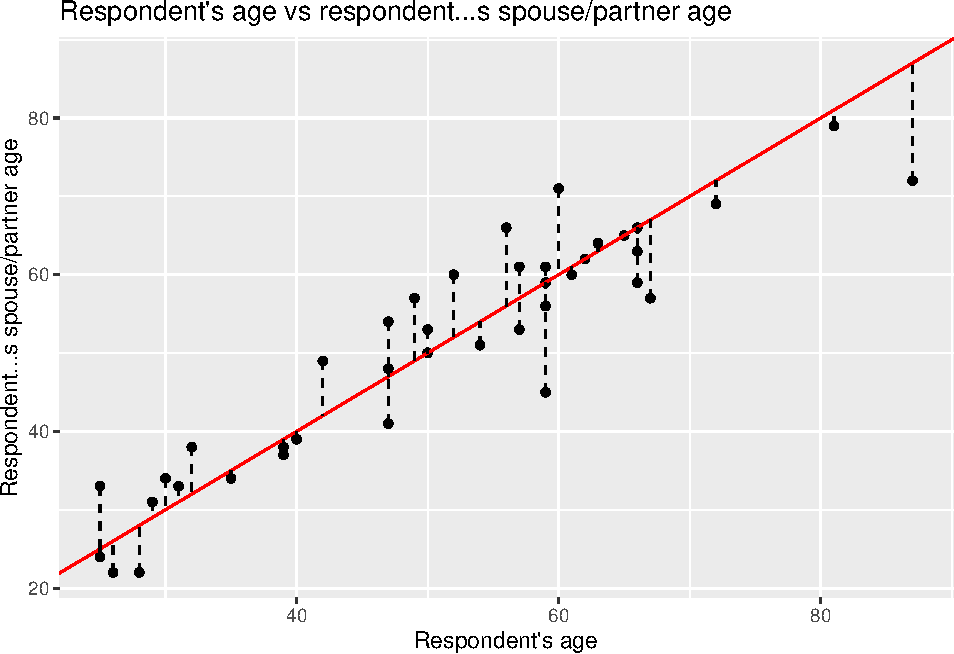
\includegraphics[width=1\linewidth]{lab-workbook_files/figure-latex/unnamed-chunk-88-1} \end{flushleft}

This distance difference is known as the residual or the error and it is often expressed with the Greek letter \(\epsilon\) (epsilon). Numerically, we can calculate this by computing the difference between the known value (the observed) and the \emph{guessed} number. Formally, the guessed number is called the expected value (also known as predicted/estimated value). Normally, the expected values in statistics are represented by putting a hat like this \(\hat{}\) on the letters. Since the independent variable is usually located on the Y axis, the expected value is differentiated from the observed values by putting the hat on the Y like this: \(\hat{y}\) (y-hat).

Let's estimate the residuals for each of the observations by subtracting \(\hat{y}_i\) from \(y_i\) (\texttt{spage} - \texttt{line1}) and store it in a column called \texttt{residuals}. Print the head of the data set after.

\begin{Shaded}
\begin{Highlighting}[]
\CommentTok{\# estimate residuals}
\NormalTok{nilt\_sample }\OtherTok{\textless{}{-}}\NormalTok{ nilt\_sample }\SpecialCharTok{\%\textgreater{}\%} 
  \FunctionTok{mutate}\NormalTok{(}\AttributeTok{residuals =}\NormalTok{ spage }\SpecialCharTok{{-}}\NormalTok{ line1)}
\CommentTok{\# print first 6 values}
\FunctionTok{head}\NormalTok{(nilt\_sample)}
\end{Highlighting}
\end{Shaded}

\begin{verbatim}
## # A tibble: 6 x 4
##    rage spage     line1 residuals
##   <dbl> <dbl+lbl> <dbl>     <dbl>
## 1    40 39           40        -1
## 2    54 51           54        -3
## 3    66 59           66        -7
## 4    60 71           60        11
## 5    35 34           35        -1
## 6    67 57           67       -10
\end{verbatim}

Coming back to the question, is my line good enough? We could sum all these residuals as an overall measure to know how good my line is. From the previous plot, we see that some of the expected ages exceed the actual values and others are below. This produces negative and positive residuals. If we simply sum them, they would compensate each other and this would not tell us much about the overall magnitude of the difference. To overcome this, we can multiply the differences by themselves (to make all numbers positive) and then sum them all together. This is known as the \emph{sum of squared residuals} (SSR) and we can use this as the criterion to measure how good my line is with respect to the overall trend of the points.

For line 1, we can easily calculate the SSR as follows:

\begin{Shaded}
\begin{Highlighting}[]
\FunctionTok{sum}\NormalTok{((nilt\_sample}\SpecialCharTok{$}\NormalTok{residuals) }\SpecialCharTok{\^{}} \DecValTok{2}\NormalTok{)}
\end{Highlighting}
\end{Shaded}

\begin{verbatim}
## [1] 1325
\end{verbatim}

The sum of squared residuals for line 1 is 1,325.

We can try different lines to find the combination of intercept and slope that produces the smallest error (SSR). To our luck, we can find the best values using a well established technique called \emph{Ordinary Least Squares} (OLS). This technique finds the optimal solution by the principle of maxima and minima. We do not need to know the details for now. The important thing is that this procedure guarantees to find a line that produces the smallest possible error (SSR).

In \texttt{R}, it is very simple to fit a linear model and we do not need to go through each of the steps above \emph{manually} nor to memorise all the steps. To do this, simply use the function \texttt{lm()}, save the result in an object called \texttt{m1} and print it.

\begin{Shaded}
\begin{Highlighting}[]
\NormalTok{m1 }\OtherTok{\textless{}{-}} \FunctionTok{lm}\NormalTok{(spage }\SpecialCharTok{\textasciitilde{}}\NormalTok{ rage, nilt\_sample)}
\NormalTok{m1}
\end{Highlighting}
\end{Shaded}

\begin{verbatim}
## 
## Call:
## lm(formula = spage ~ rage, data = nilt_sample)
## 
## Coefficients:
## (Intercept)         rage  
##       6.299        0.875
\end{verbatim}

So, this is the optimal intercept \(\beta_0\) and slope \(\beta_1\) that produces the least sum of the square. Let's see what the SSR is compared to my arbitrary guess above:

\begin{Shaded}
\begin{Highlighting}[]
\FunctionTok{sum}\NormalTok{(}\FunctionTok{residuals}\NormalTok{(m1) }\SpecialCharTok{\^{}} \DecValTok{2}\NormalTok{)}
\end{Highlighting}
\end{Shaded}

\begin{verbatim}
## [1] 1175.209
\end{verbatim}

Yes, this is better than before (because the value is smaller)!

Let's plot the line we guessed and the optimal line together:

\begin{Shaded}
\begin{Highlighting}[]
\FunctionTok{ggplot}\NormalTok{(nilt\_sample, }\FunctionTok{aes}\NormalTok{(}\AttributeTok{x =}\NormalTok{ rage, }\AttributeTok{y =}\NormalTok{ spage)) }\SpecialCharTok{+} 
  \FunctionTok{geom\_point}\NormalTok{() }\SpecialCharTok{+}
  \FunctionTok{geom\_abline}\NormalTok{(}\AttributeTok{slope =} \DecValTok{1}\NormalTok{, }\AttributeTok{intercept =} \DecValTok{0}\NormalTok{, }\AttributeTok{colour =} \StringTok{"red"}\NormalTok{) }\SpecialCharTok{+}
  \FunctionTok{geom\_smooth}\NormalTok{(}\AttributeTok{method =} \StringTok{"lm"}\NormalTok{, }\AttributeTok{se =} \ConstantTok{FALSE}\NormalTok{) }\SpecialCharTok{+}
   \FunctionTok{labs}\NormalTok{(}\AttributeTok{title =} \StringTok{"Respondent\textquotesingle{}s age vs respondent’s spouse/partner age"}\NormalTok{, }
       \AttributeTok{x =} \StringTok{"Respondent\textquotesingle{}s age"}\NormalTok{, }\AttributeTok{y =} \StringTok{"Respondent’s spouse/partner age"}\NormalTok{ )}
\end{Highlighting}
\end{Shaded}

\begin{flushleft}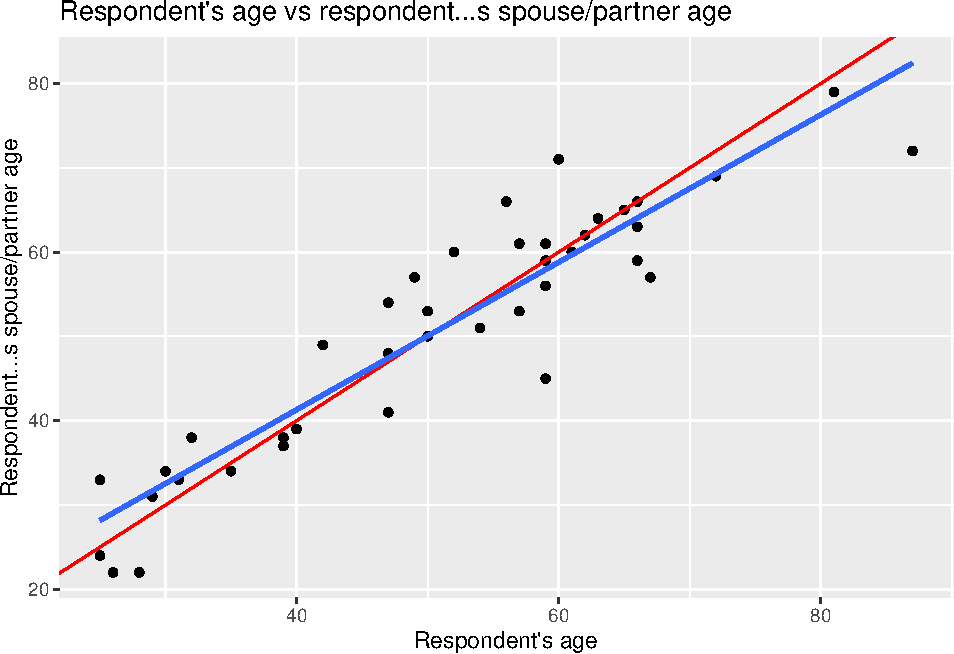
\includegraphics[width=1\linewidth]{lab-workbook_files/figure-latex/unnamed-chunk-93-1} \end{flushleft}

The blue is the optimal solution, whereas the red was just an arbitrary guess. We can see that the optimal is more balanced than the red in relation to the observed data points.

\hypertarget{formal-specification}{%
\subsection{Formal specification}\label{formal-specification}}

Now you are ready for the the formal specification of the linear model. After the introduction above, it is easy to take the pieces apart. In essence, the simple linear model is telling us that the dependent value \(y\) is defined by a line that intersects the vertical axis at \(\beta_0\), plus the multiplication of the slope \(\beta_1\) by the value of \(x_1\), plus some residual \(\epsilon\). The second part of the equation is just telling us that the residuals are normally distributed (that is when a histogram of the residuals follows a bell-shaped curve).

\[
\begin{align}
y = \beta_0 + \beta_1 * x_1 + \epsilon, && \epsilon ~ N(0, \sigma)  
\end{align}
\]

You do not need to memorize this equation, but being familiar to this type of notation will help you to expand your skills in quantitative research.

\hypertarget{fitting-linear-regression-in-r}{%
\section{Fitting linear regression in R}\label{fitting-linear-regression-in-r}}

\hypertarget{r-syntax}{%
\subsection{R syntax}\label{r-syntax}}

We already fitted our first linear model using the \texttt{lm()} above, which of course stands for \emph{linear model}, but we did not discuss the specifications needed in this function. The first argument takes the dependent variable, then, we use tilde \texttt{\textasciitilde{}} to express that this is \emph{followed by} the independent variable. Then, we specify the data set separated by a comma, as shown below (this is just a conceptual example, it does not actually run!):

\begin{Shaded}
\begin{Highlighting}[]
\FunctionTok{lm}\NormalTok{(dependent\_variable }\SpecialCharTok{\textasciitilde{}}\NormalTok{ independent\_variable, data)}
\end{Highlighting}
\end{Shaded}

\hypertarget{running-a-simple-linear-regression}{%
\subsection{Running a simple linear regression}\label{running-a-simple-linear-regression}}

Now, let's try with the full data set. First, we will fit a linear model using the same variables as the example above but including all the observations (remember that before we were working only with a small random sample). The first argument is the respondent's spouse/partner age \texttt{spage}, followed by the respondent's age \texttt{rage}. Let's assign the model to an object called \texttt{m2} and print it after.

\begin{Shaded}
\begin{Highlighting}[]
\NormalTok{m2 }\OtherTok{\textless{}{-}} \FunctionTok{lm}\NormalTok{(spage }\SpecialCharTok{\textasciitilde{}}\NormalTok{ rage, nilt)}
\NormalTok{m2}
\end{Highlighting}
\end{Shaded}

\begin{verbatim}
## 
## Call:
## lm(formula = spage ~ rage, data = nilt)
## 
## Coefficients:
## (Intercept)         rage  
##      3.7039       0.9287
\end{verbatim}

The output first displays the formula employed to estimate the model. Then, it show us the estimated values for the intercept and the slope for the age of the respondent, these estimated values are called coefficients. In this model, the coefficients differ from the ones in the example above (m1). This is because we now have more information to fit this line. Despite the difference, we see that the relationship is still in the same direction (positive). In fact, the value of the slope \(\beta_1\) did not change much if you look at it carefully (0.87 vs 0.92).

\hypertarget{interpreting-results}{%
\subsection{Interpreting results}\label{interpreting-results}}

But what are the slope and intercept telling us? The first thing to note is that the slope is positive, which means that the relationship between the respondent age and their partner are in the same direction. When the age of the respondent goes up, the age of their partner is expected to go up as well.

In our model, the intercept does not have a meaningful interpretation on its own, it would not be logical to say that when the respondent's age is 0 their partner would be expected to be 3.70 years old. Interpretations should be made only within the range of the values used to fit the model (the youngest age in this data set is 18). The slope can be interpreted as following: For every year older the respondent is, the partner's age is expected to change by 0.92. In other words, the respondents are expected to have a partner who is 0.92 times years older than themselves. This means that their partners are expected to be slightly younger.

In this case, the units of the dependent variable are the same as the independent (age vs age) which make it easy to interpret. In reality, there might be more factors that potentially affect how people select their partners (e.g.~genders, education, race/ethnicity, etc.). For now, we are keeping things simple using only these two variables.

Let's practice with another example. What if we are interested in income? We can use personal income \texttt{persinc2} as the dependent variable and the number of hours worked a week \texttt{rhourswk} as the independent variable. We'll assign the result to an object called \texttt{m3}.

\begin{Shaded}
\begin{Highlighting}[]
\NormalTok{m3 }\OtherTok{\textless{}{-}} \FunctionTok{lm}\NormalTok{(persinc2 }\SpecialCharTok{\textasciitilde{}}\NormalTok{ rhourswk, }\AttributeTok{data =}\NormalTok{ nilt)}
\NormalTok{m3}
\end{Highlighting}
\end{Shaded}

\begin{verbatim}
## 
## Call:
## lm(formula = persinc2 ~ rhourswk, data = nilt)
## 
## Coefficients:
## (Intercept)     rhourswk  
##      5170.4        463.2
\end{verbatim}

This time, the coefficients look quite different. The results are telling us that for every additional hour worked a week a respondent is expected to earn £463.2 more a year than other respondent. Note that the input units are not the same in the interpretation. The dependent variable is in pounds earned a year and the independent is in hours worked a week. Does this mean that someone who works 0 hours a week is expected to earn £5170.4 a year (given the fitted model \(\hat{persinc2} = 5170.4 + 0*463.2\)) or that someone who works 110 hours a week (impossible!) is expected to earn £56K a year? We should only make reasonable interpretations of the coefficients within the range analysed.

Finally, an important thing to know when interpreting linear models using cross sectional data (data collected in a single time point only) is: \textbf{\emph{correlation does not imply causation}}. Variables are often correlated with other non-observed variables which may cause the effects observed on the independent variable in reality. This is why we cannot always be sure that X is causing the observed changes on Y.

\hypertarget{model-evaluation}{%
\section{Model evaluation}\label{model-evaluation}}

In the next section, we suggest you to focus on the interpretation of the results of the linear model. You do not need to reproduce the code.

\hypertarget{model-summary}{%
\subsection{Model summary}\label{model-summary}}

So far, we have talked about the basics of the linear model. If we print a summary of the model, we can obtain more information to evaluate it.

\begin{Shaded}
\begin{Highlighting}[]
\FunctionTok{summary}\NormalTok{(m2)}
\end{Highlighting}
\end{Shaded}

\begin{verbatim}
## 
## Call:
## lm(formula = spage ~ rage, data = nilt)
## 
## Residuals:
##     Min      1Q  Median      3Q     Max 
## -33.211  -2.494   0.075   2.505  17.578 
## 
## Coefficients:
##             Estimate Std. Error t value Pr(>|t|)    
## (Intercept)  3.70389    0.66566   5.564    4e-08 ***
## rage         0.92869    0.01283  72.386   <2e-16 ***
## ---
## Signif. codes:  0 '***' 0.001 '**' 0.01 '*' 0.05 '.' 0.1 ' ' 1
## 
## Residual standard error: 4.898 on 589 degrees of freedom
##   (613 observations deleted due to missingness)
## Multiple R-squared:  0.8989, Adjusted R-squared:  0.8988 
## F-statistic:  5240 on 1 and 589 DF,  p-value: < 2.2e-16
\end{verbatim}

There are a lot of numbers from the result. Let's break down the information into different pieces: first the call, second the residuals, third the coefficients, and fourth the goodness-of-fit measures, as shown below:

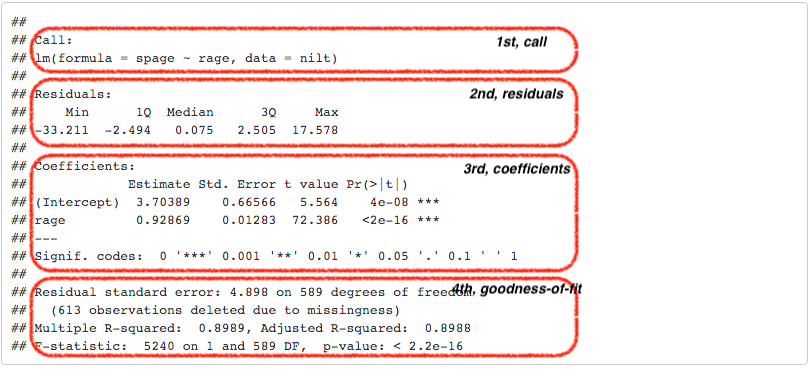
\includegraphics{./images/r_studio_lab6_model_summary.png}
The first part, \textbf{Call}, is simply printing the variables that were used to produce the models.

The second part, the \textbf{Residuals}, provides a small summary of the residuals by quartile, including minimum and maximum residual values. Remember the second part of the formal specification of the model? Well, this is where we can see in practice the distribution of the residuals. If we look at the first and third quartile, we can see that that 50\% of the predicted values by the model are \(\pm\) 2.5 years old away form the observed partner's age\ldots not that bad.

The third part is about the \textbf{coefficients}. This time, the summary provides more information about the intercept and the slope than just the estimated coefficients as before. Usually, we focus on the independent variables in this section, \texttt{rage} in our case. The second column, standard error, tell us how large the error of the slope is, which is small for our variable. The third and fourth columns provide measures about the statistical significance of the relationship between the dependent and independent variable. The most commonly reported is the p-value (the fourth column). When these values contains many digits, R reports the result in scientific notation. In our result the p-value is \texttt{\textless{}2e-16} (the real equivalent number is \textless0.0000000000000002, if you want to know more about scientific notation click \href{https://www.calculatorsoup.com/calculators/math/scientific-notation-converter.php\#:~:text=The\%20proper\%20format\%20for\%20scientific,equivalent\%20to\%20the\%20original\%20number.}{here}). As a general agreed principle, \textbf{if the p-value is equal or less than 0.05 (\(p\) ≤ 0.05), we can reject the null hypothesis, and say that the relationship between the dependent variable and the independent is significant.} In our case, the p-value is far lower than 0.05. So, we can say that the relationship between the respondent's spouse/partner age and the respondent's age is significant. In fact, R includes codes for each coefficient to help us to identify the significance. In our result, we got three stars/asterisks. This is because the value is less than 0.001. R assigns two stars if the p-value is less than 0.01, and one star if it is lower than 0.05.

In the fourth area, we have various goodness-of-fit measures. Overall, these measures tell us how well the model represents our data. For now, let's focus on the \emph{adjusted r-squared} and the sample size. The r-squared is a value that goes from 0 to 1. 0 means that model is not explaining any of the variance, whereas 1 would mean a perfect model. In social sciences we do not see high values often. The adjusted r-squared can be understood as the percentage variance that the model is able to explain. In the example above, the model explains 89.88\% percent of the total variance. This is a good fit, but this is because we are modelling a quite ``obvious'' relationship. The r-squared does not represent how good or bad our work is. You may wonder why we do not report the sum of squared residuals (SSR), as we just learned. This is because the scale of the SSR is in the units used to fit the model, which would make it difficult to compare our model with other models that use different units or different variables. Conversely, the adjusted r-squared is expressed in relative terms which makes it a more suitable measure to compare with other models. An important thing to note is that the output is telling us that this model excluded 613 observations which were missing in our dataset. This is because we do not have the age of the respondent's partner in 613 of the rows. This missingness may be because the respondent do not have a partner, refused to provide the information, etc.

In academic papers in the social sciences, usually the measures reported are the coefficients, p-values, the adjusted r-squared, and the size of the sample used to fit the model (number of observations).

\hypertarget{further-checks}{%
\subsection{Further checks}\label{further-checks}}

The linear model, as many other techniques in statistics, relies on assumptions. These refer to characteristics of the data that are taken for granted to generate the estimates. It is the task of the modeller/analyst to make sure the data used follows these assumptions. One simple yet important check is to examine the distribution of the residuals, which ought to follow a normal distribution.

Does the residuals follow a normal distribution in \texttt{m1}? We can go further and plot a histogram to graphically evaluate it. Use the function \texttt{residuals()} to extract the residuals from our object \texttt{m2}, and then plot a histogram with the r-base function \texttt{hist()}.

\begin{Shaded}
\begin{Highlighting}[]
\FunctionTok{hist}\NormalTok{(}\FunctionTok{residuals}\NormalTok{(m2), }\AttributeTok{breaks =} \DecValTok{20}\NormalTok{)}
\end{Highlighting}
\end{Shaded}

\begin{flushleft}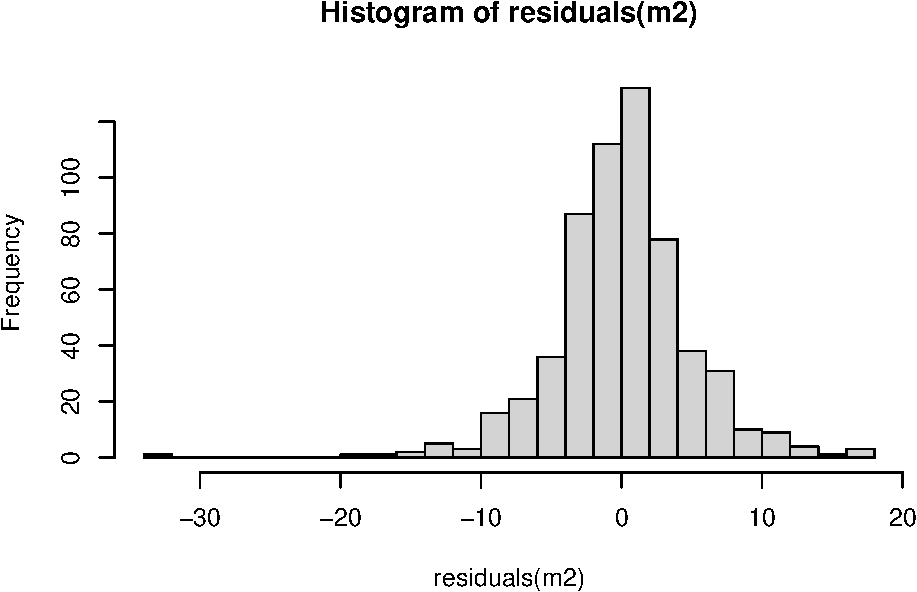
\includegraphics[width=1\linewidth]{lab-workbook_files/figure-latex/unnamed-chunk-98-1} \end{flushleft}

Overall, it seems that the residuals follow the normal distribution reasonably well, with the exception of the negative value to the left of the plot. Very often when there is a strange distribution or different to the normal is because one of the assumptions is violated. If that is the case we cannot trust the coefficient estimates. In the next lab we will talk more about the assumptions of the linear model. For now, we will leave it here and get some practice.

\hypertarget{lab-activities}{%
\section{Lab activities}\label{lab-activities}}

In the \texttt{linear\_model\_intro.R} script, use the \texttt{nilt} dataset in to:

\begin{enumerate}
\def\labelenumi{\arabic{enumi}.}
\tightlist
\item
  Plot a scatter plot using \texttt{ggplot}. In the aesthetics, locate \texttt{rhourswk} in the X axis, and \texttt{persinc2} in the Y axis. In the \texttt{geom\_point()} jitter the points by specifying the \texttt{position\ =\ \textquotesingle{}jitter\textquotesingle{}}. Also, include the best fit line using the \texttt{geom\_smooth()} function, and specify the \texttt{method\ =\ \textquotesingle{}lm\textquotesingle{}} inside.
\item
  Print the summary of \texttt{m3} using the \texttt{summary()} function.
\item
  Is the the relationship of hours worked a week significant?
\item
  What is the adjusted r-squared? How would you interpret it?
\item
  What is the sample size to fit the model?
\item
  What is the expected income in pounds a year for a respondent who works 30 hours a week according to coefficients of this model?
\item
  Plot a histogram of the residuals of \texttt{m3} using the \texttt{residuals()} function inside \texttt{hist()}. Do the residuals look normally distributed (as in a bell-shaped curve)?
\item
  Discuss your answers with your neighbour or tutor.
\end{enumerate}

\hypertarget{multi-lm}{%
\chapter{Multivariate linear model}\label{multi-lm}}

\hypertarget{introduction-2}{%
\section{Introduction}\label{introduction-2}}

In the last lab we mentioned that one of the advantages of linear regression is that we can include more than one independent (explanatory) variable to evaluate their relationship with the dependent variable. This technique is known as multivariate linear regression. In practice, few studies in quantitative social research rely only on simple linear models. This is because often in reality there is more than one variable associated to a social phenomenon. This is why it is important to familiarise yourself with the multivariate linear model.

\hypertarget{multivariate-model}{%
\section{Multivariate model}\label{multivariate-model}}

The multivariate linear model is based on the same principles as the simple linear model. It is worth remembering that this model is appropriate only when we have a numeric (interval/ratio) dependent variable. As a rule-of-thumb, a variable can be treated as numeric when you have at least 7 ordered categories (Fogarty, 2019). As mentioned before, we can use any type of independent variables, such as ordinal, categorical and numeric. More than one and a combination of these can be analysed simultaneously.

\hypertarget{paralell-slopes}{%
\subsection{Paralell slopes}\label{paralell-slopes}}

We will follow-up with the example we used before introducing the simple linear model to further illustrate the advantages of using more than one variable. To do so, please set your RStudio environment as follows:

\begin{enumerate}
\def\labelenumi{\arabic{enumi}.}
\tightlist
\item
  Go to your `Quants lab group' in \href{https://rstudio.cloud/}{RStudio Cloud};
\item
  Open your own `NILT2' project from your `Quants lab group';
\item
  Once in the project, create a new R Script file (a simple R Script, NOT an \texttt{.Rmd} file).
\item
  Save the script document as `multivariate\_linear\_model'.
\end{enumerate}

Reproduce the code below, by copying, pasting and running it from your new script.

First, install the \texttt{moderndive}package.

\begin{Shaded}
\begin{Highlighting}[]
\FunctionTok{install.packages}\NormalTok{(}\StringTok{"moderndive"}\NormalTok{)}
\end{Highlighting}
\end{Shaded}

Load the \texttt{tidyverse} and \texttt{moderndive} libraries (\texttt{tidyverse} was pre-installed for you before, you do not need to re-install it in this project) and read the \texttt{nilt\_r\_object.rds} file which is stored in the `data' folder and contains the NILT survey.

\begin{Shaded}
\begin{Highlighting}[]
\DocumentationTok{\#\# Load the packages}
\FunctionTok{library}\NormalTok{(tidyverse)}
\FunctionTok{library}\NormalTok{(moderndive)}

\CommentTok{\# Read the data from the .rds file}
\NormalTok{nilt }\OtherTok{\textless{}{-}} \FunctionTok{readRDS}\NormalTok{(}\StringTok{"data/nilt\_r\_object.rds"}\NormalTok{)}
\end{Highlighting}
\end{Shaded}

Once again, create a minimal random sample for the following example using the code below:

\begin{Shaded}
\begin{Highlighting}[]
\CommentTok{\# select a small random sample}
\FunctionTok{set.seed}\NormalTok{(}\DecValTok{3}\NormalTok{)}
\CommentTok{\# Filter where partner\textquotesingle{}s age is not NA and take a random sample of 40}
\NormalTok{nilt\_sample }\OtherTok{\textless{}{-}} \FunctionTok{filter}\NormalTok{(nilt, }\SpecialCharTok{!}\FunctionTok{is.na}\NormalTok{(spage)) }\SpecialCharTok{\%\textgreater{}\%} \FunctionTok{sample\_n}\NormalTok{(}\DecValTok{40}\NormalTok{)}
\CommentTok{\# Select only respondent\textquotesingle{}s age and spouse/partner\textquotesingle{}s age}
\NormalTok{nilt\_sample }\OtherTok{\textless{}{-}} \FunctionTok{select}\NormalTok{(nilt\_sample, rage, spage, rsex)}
\end{Highlighting}
\end{Shaded}

As a follow-up, we will draw a scatter plot using \texttt{ggplot} specifying the age of the respondent \texttt{rage} on the X axis and the respondent's partner/spouse age \texttt{spage} on the Y axis. This time, we will add sex \texttt{rsex} as a third variable defining the \texttt{color} argument.

\begin{Shaded}
\begin{Highlighting}[]
\CommentTok{\# plot}
\FunctionTok{ggplot}\NormalTok{(nilt\_sample,  }\FunctionTok{aes}\NormalTok{(}\AttributeTok{x =}\NormalTok{ rage, }\AttributeTok{y =}\NormalTok{ spage, }\AttributeTok{color =}\NormalTok{ rsex)) }\SpecialCharTok{+} 
  \FunctionTok{geom\_point}\NormalTok{(}\AttributeTok{position =} \StringTok{"jitter"}\NormalTok{) }\SpecialCharTok{+}
  \FunctionTok{labs}\NormalTok{(}\AttributeTok{title =} \StringTok{"Respondent\textquotesingle{}s age vs respondent’s spouse/partner age"}\NormalTok{, }
       \AttributeTok{x =} \StringTok{"Respondent\textquotesingle{}s age"}\NormalTok{, }\AttributeTok{y =} \StringTok{"Respondent’s spouse/partner age"}\NormalTok{ )}
\end{Highlighting}
\end{Shaded}

\begin{flushleft}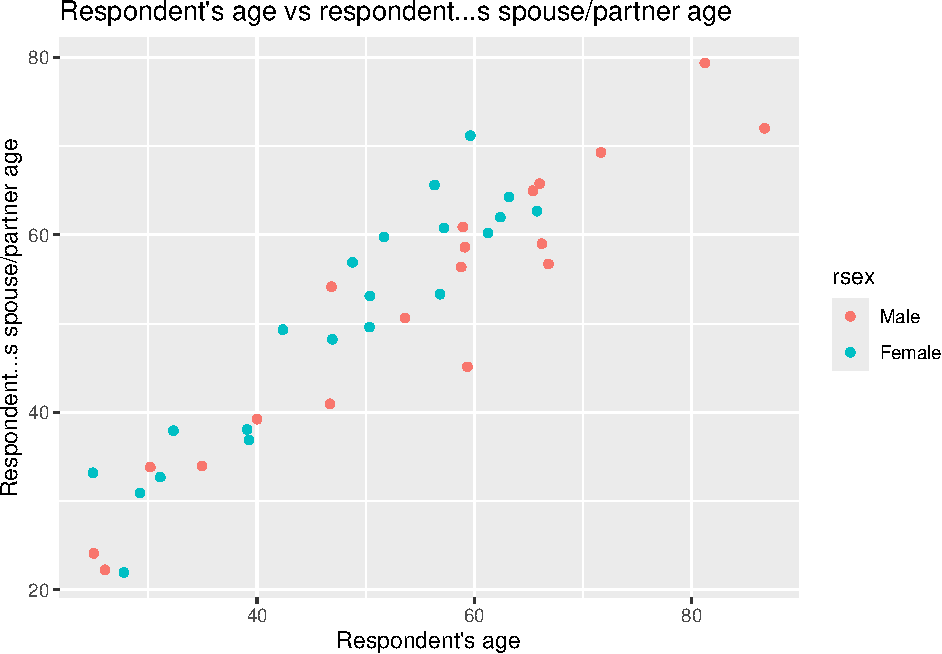
\includegraphics[width=1\linewidth]{lab-workbook_files/figure-latex/unnamed-chunk-102-1} \end{flushleft}

What do you observe in the plot above? \ldots{}

The first thing to note is that females and males go in the same direction. When the respondent's age increases the age of the partner increases as well. An interesting thing is that females tend to be located higher with respect to the Y axis compared to the male dots.

Therefore, we can imagine that not only the age of the respondent is involved in the decision on how people choose their partner, but also the respondents' sex. We can draw two lines, one for male and the other for female respondents, instead of only a general one as we did in the previous lab. To do this we will use the \texttt{ggplot} function in combination with the \texttt{geom\_parallel\_slopes} function from the \texttt{moderndive} package:

\begin{Shaded}
\begin{Highlighting}[]
\CommentTok{\# plot}
\FunctionTok{ggplot}\NormalTok{(nilt\_sample,  }\FunctionTok{aes}\NormalTok{(}\AttributeTok{x =}\NormalTok{ rage, }\AttributeTok{y =}\NormalTok{ spage, }\AttributeTok{color =}\NormalTok{ rsex)) }\SpecialCharTok{+} 
  \FunctionTok{geom\_point}\NormalTok{(}\AttributeTok{position =} \StringTok{"jitter"}\NormalTok{) }\SpecialCharTok{+}
  \FunctionTok{geom\_parallel\_slopes}\NormalTok{(}\AttributeTok{se =} \ConstantTok{FALSE}\NormalTok{) }\SpecialCharTok{+}
  \FunctionTok{labs}\NormalTok{(}\AttributeTok{title =} \StringTok{"Respondent\textquotesingle{}s age vs respondent’s spouse/partner age"}\NormalTok{, }
       \AttributeTok{x =} \StringTok{"Respondent\textquotesingle{}s age"}\NormalTok{, }\AttributeTok{y =} \StringTok{"Respondent’s spouse/partner age"}\NormalTok{ )}
\end{Highlighting}
\end{Shaded}

\begin{flushleft}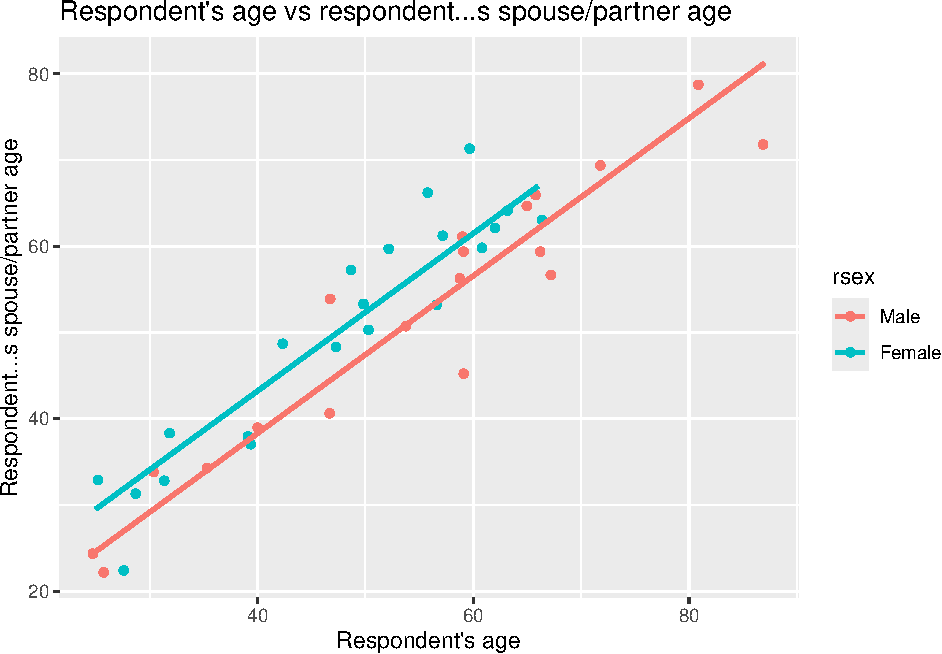
\includegraphics[width=1\linewidth]{lab-workbook_files/figure-latex/unnamed-chunk-103-1} \end{flushleft}

Well, our suspicion that the points representing female respondents were generally above the male ones is turning out to be true. What we have in the plot above are the optimal parallel lines that describe our points the best for each group. The interpretation of our visualizations so far is:

\begin{enumerate}
\def\labelenumi{\arabic{enumi}.}
\tightlist
\item
  both males and females partner's age is positively associated with respondent's age.
\item
  This association is different for males and females. Overall, females choose older partners compared to males.
\end{enumerate}

But what is the magnitude of these relationships? We can easily extend the simple linear model by adding \texttt{rsex} as a second explanatory variable as follows:

\begin{Shaded}
\begin{Highlighting}[]
\NormalTok{m1 }\OtherTok{\textless{}{-}} \FunctionTok{lm}\NormalTok{(spage }\SpecialCharTok{\textasciitilde{}}\NormalTok{ rage }\SpecialCharTok{+}\NormalTok{ rsex, nilt\_sample)}
\NormalTok{m1}
\end{Highlighting}
\end{Shaded}

\begin{verbatim}
## 
## Call:
## lm(formula = spage ~ rage + rsex, data = nilt_sample)
## 
## Coefficients:
## (Intercept)         rage   rsexFemale  
##      1.7383       0.9138       4.9190
\end{verbatim}

From the output, we see that there is one intercept \(\beta_0\), one slope coefficient \(\beta_1\) for the numeric variable \texttt{rage}, and another coefficient \(\beta_2\) for the categorical variable. If you observe closer, the output appended only one of the two categories for \texttt{rsex}. This is because categorical variables take one of the categories as the reference. The variable that is not shown is the reference, `Male', in this case.

Being more precise with our previous interpretation, we can say there is a positive relationship between both males and female participants' age and their partner's age by a factor of 0.91 for every additional year in age. Also, female respondent's partners are expected to be 4.9 years older compared to male respondents.

Before we move on, it is worth mentioning that the criterion to fit the coefficient is the same as in the linear model. This procedure guarantees to produce the smallest possible sum of squared residuals (SSR) using the ordinary least square method (OLS). We can check if the SSR was reduced by adding this extra variable by computing the SSR as we did before:

\begin{Shaded}
\begin{Highlighting}[]
\FunctionTok{sum}\NormalTok{(}\FunctionTok{residuals}\NormalTok{(m1) }\SpecialCharTok{\^{}} \DecValTok{2}\NormalTok{)}
\end{Highlighting}
\end{Shaded}

\begin{verbatim}
## [1] 948.263
\end{verbatim}

Yes, it improved! Before, it was about 1,175, as we saw in the last lab workbook.

\hypertarget{multivariate-model-specification}{%
\subsection{Multivariate model specification}\label{multivariate-model-specification}}

After the introduction of the simple linear model, the formal definition of the multivariate linear model should not look that scary, right? In essence, this equation tells us how \(\hat{y}\) is described/explained by other variables.

\[
\begin{aligned}
\hat{y} = \hat{\beta_0} + \hat{\beta_1}*x_1 + \hat{\beta_2}*x_2 + ... +  \hat{\epsilon}, && \epsilon ~ N(0, \sigma)  
\end{aligned}
\]

We can break down the equation above in smaller pieces as follows:

\begin{itemize}
\tightlist
\item
  \(\hat{y}\) is the dependent variable, which is explained by
\item
  \(\hat{\beta_0}\) the intercept, plus
\item
  \(\hat{\beta_1}\) the slope coefficient for the first independent variable times the value of \(x_1\) variable 1, plus
\item
  \(\hat{\beta_2}\) the slope coefficient for the second independent variable times the value of \(x_2\), plus
\item
  \(...\) any number of independent variables, plus
\item
  \(\hat{\epsilon}\) the error/residual term.
\item
  \(\epsilon ~ N(0, \sigma)\) this bit tell us that the residuals are normally distributed.
\end{itemize}

\hypertarget{r-syntax-for-the-multivariate-linear-model}{%
\section{R syntax for the multivariate linear model}\label{r-syntax-for-the-multivariate-linear-model}}

(You don't need to reproduce the code of this section in your script).

The general syntax in R is as follows:

\begin{Shaded}
\begin{Highlighting}[]
\FunctionTok{lm}\NormalTok{(formula, data)}
\end{Highlighting}
\end{Shaded}

Where the formula is given by a dependent variable which is followed by \texttt{\textasciitilde{}} one or more independent variables joined by a plus sign \texttt{+}:

\begin{Shaded}
\begin{Highlighting}[]
\NormalTok{dependent\_variable }\SpecialCharTok{\textasciitilde{}}\NormalTok{ independent\_variable1 }\SpecialCharTok{+}\NormalTok{ independent\_variable2 ...}
\end{Highlighting}
\end{Shaded}

In the previous section, we used a small random sample of 40 people only. Now, let's fit a multivariate linear model using all the observations in the \texttt{nilt} dataset. In addition to the respondent age \texttt{rage} and \texttt{rsex}, we might be interested to know whether the type of place where they live (e.g.~big city, village, farm/country, etc.) \texttt{placeliv} plays a role in how people choose their partner.

First, we need to coerce the \texttt{placeliv} variable as factor. And we will have a quick look at a table of this variable to have an idea of how respondents are distributed and see how the factor levels are ordered.

\begin{Shaded}
\begin{Highlighting}[]
\CommentTok{\# Coerce to factor}
\NormalTok{nilt }\OtherTok{\textless{}{-}}\NormalTok{ nilt }\SpecialCharTok{\%\textgreater{}\%} 
  \FunctionTok{mutate}\NormalTok{(}\AttributeTok{placeliv =} \FunctionTok{as\_factor}\NormalTok{(placeliv))}
\CommentTok{\# Create table}
\FunctionTok{table}\NormalTok{(nilt}\SpecialCharTok{$}\NormalTok{placeliv)}
\end{Highlighting}
\end{Shaded}

\begin{verbatim}
## 
##                              Dont know                          ...a big city 
##                                      0                                    168 
## the suburbs or outskirts of a big city                   a small city or town 
##                                    233                                    477 
##                      a country village          a farm or home in the country 
##                                    176                                    146
\end{verbatim}

We see that most of the respondents live in `a small city or town'. Also, note that the category `Dont know' contains 0 observations. Let's use the function \texttt{droplevels()} to remove the unused category in our variables. This also means that the first level in this variable will be `a big city'. Then, we will fit the model and store it in an object called \texttt{m2}.

\begin{Shaded}
\begin{Highlighting}[]
\CommentTok{\# remove unused levels}
\NormalTok{nilt }\OtherTok{\textless{}{-}} \FunctionTok{droplevels}\NormalTok{(nilt)}
\CommentTok{\# boxplot}
\NormalTok{m2 }\OtherTok{\textless{}{-}} \FunctionTok{lm}\NormalTok{(spage }\SpecialCharTok{\textasciitilde{}}\NormalTok{ rage }\SpecialCharTok{+}\NormalTok{ rsex }\SpecialCharTok{+}\NormalTok{ placeliv, nilt)}
\NormalTok{m2}
\end{Highlighting}
\end{Shaded}

\begin{verbatim}
## 
## Call:
## lm(formula = spage ~ rage + rsex + placeliv, data = nilt)
## 
## Coefficients:
##                                    (Intercept)  
##                                        1.34251  
##                                           rage  
##                                        0.94147  
##                                     rsexFemale  
##                                        3.79426  
## placelivthe suburbs or outskirts of a big city  
##                                        0.02099  
##                   placeliva small city or town  
##                                       -0.71196  
##                      placeliva country village  
##                                        0.25645  
##          placeliva farm or home in the country  
##                                       -0.01280
\end{verbatim}

From the result:

\begin{enumerate}
\def\labelenumi{\arabic{enumi}.}
\tightlist
\item
  We confirm the positive relationship between the respondent's age and their partner by a factor of 0.94.
\item
  The difference in years by sex now is smaller. We see that the age of a female respondent's partner is expected to be 3.8 years older compared to males.
\item
  As before, we see that the result appended the name of the categories to the \texttt{placeliv} variables. This is because it is comparing each of the categories with the category of reference, in this case, `a big city'. The interpretation must be in comparative terms. For instance, the age of the respondent's partner in `the suburbs or outskirts of a big city' is expected to be 0.02 years older than the partner of someone living in a `a big city'. Overall, the coefficients do not differ much as a function of the type of place of where they live. The largest expected difference is for people living in `a small city or town', where partner's age is expected to be -0.7 years old compared to those living in `a big city'.
\end{enumerate}

In general, our model can be expressed as:

\[ \hat{spage}_i = \hat{\beta_0} + \hat{\beta_1}*rage_i + \hat{\beta_2}*rsex_i + \hat{\beta_3} *  placeliv_i \]
So, if we wanted to know the expected age of the partner of a 40 years old female who lives in a small city or town, we can use and apply the formula above:

\begin{Shaded}
\begin{Highlighting}[]
\FloatTok{1.34} \SpecialCharTok{+} \FloatTok{0.94}\SpecialCharTok{*}\DecValTok{40} \SpecialCharTok{+} \FloatTok{3.80}\SpecialCharTok{*}\DecValTok{1} \SpecialCharTok{+} \SpecialCharTok{{-}}\FloatTok{0.7}\SpecialCharTok{*}\DecValTok{1}
\end{Highlighting}
\end{Shaded}

\begin{verbatim}
## [1] 42.04
\end{verbatim}

The expected age of a 40 year old female's partner is, therefore, 41.7 years old.

\hypertarget{model-evaluation-1}{%
\subsection{Model evaluation}\label{model-evaluation-1}}

We can obtain more details from our model using the \texttt{summary()} function.

\begin{Shaded}
\begin{Highlighting}[]
\FunctionTok{summary}\NormalTok{(m2)}
\end{Highlighting}
\end{Shaded}

\begin{verbatim}
## 
## Call:
## lm(formula = spage ~ rage + rsex + placeliv, data = nilt)
## 
## Residuals:
##     Min      1Q  Median      3Q     Max 
## -34.737  -2.176  -0.139   2.214  19.530 
## 
## Coefficients:
##                                                Estimate Std. Error t value
## (Intercept)                                     1.34251    0.86727   1.548
## rage                                            0.94147    0.01202  78.311
## rsexFemale                                      3.79426    0.37761  10.048
## placelivthe suburbs or outskirts of a big city  0.02099    0.72637   0.029
## placeliva small city or town                   -0.71196    0.65391  -1.089
## placeliva country village                       0.25645    0.75903   0.338
## placeliva farm or home in the country          -0.01280    0.75787  -0.017
##                                                Pr(>|t|)    
## (Intercept)                                       0.122    
## rage                                             <2e-16 ***
## rsexFemale                                       <2e-16 ***
## placelivthe suburbs or outskirts of a big city    0.977    
## placeliva small city or town                      0.277    
## placeliva country village                         0.736    
## placeliva farm or home in the country             0.987    
## ---
## Signif. codes:  0 '***' 0.001 '**' 0.01 '*' 0.05 '.' 0.1 ' ' 1
## 
## Residual standard error: 4.524 on 583 degrees of freedom
##   (614 observations deleted due to missingness)
## Multiple R-squared:  0.9143, Adjusted R-squared:  0.9134 
## F-statistic:  1037 on 6 and 583 DF,  p-value: < 2.2e-16
\end{verbatim}

From the summary, we note that the 1st and 3rd quartile of residuals are symmetric (-2.18 to 2.21). This means that 50\% of the estimated/predicted ages are approximately \(\pm\) 2.2 years away from the observed partner's age. Though, the minimum and the maximum residuals are not symmetric, this could be due to some extreme observed values. We can have a look to a histogram of the residuals to have a clearer idea.

\begin{Shaded}
\begin{Highlighting}[]
\FunctionTok{hist}\NormalTok{(m2}\SpecialCharTok{$}\NormalTok{residuals)}
\end{Highlighting}
\end{Shaded}

\begin{flushleft}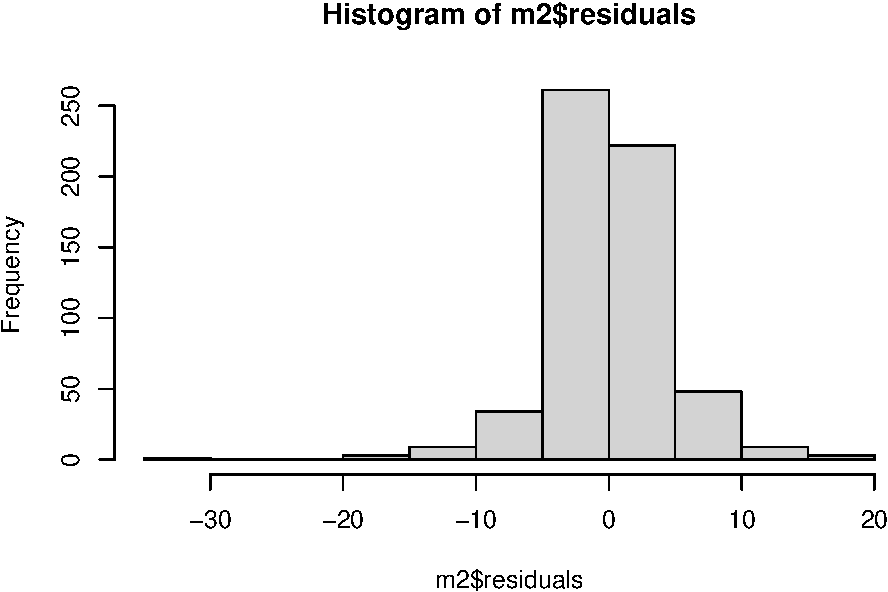
\includegraphics[width=1\linewidth]{lab-workbook_files/figure-latex/unnamed-chunk-112-1} \end{flushleft}

Overall they seem normally distributed with the exception of the negative value to the left.

Secondly, from the summary we can see that respondent age \texttt{rage} and respondent sex \texttt{rsex} have a significant association with the dependent variable (indicated by the p-value \textless{} 0.001). You can confirm this in the fourth column of the coefficients (`Pr(\textgreater\textbar t\textbar)'). Also, the std. error for the coefficients of this variables is small. However, the std. error for the categories of the place of where they live \texttt{placeliv} is large when compared to the estimated coefficients in the first column. In fact, when we look at the fourth column we see that the p-values are much larger than 0.05, which means that there is not a significant relationship between any of the type of places where they live and the partner's respondent age. What this means is that the place where people live does not play a role in the age of the respondent's partner.

Third, this time we see that the multiple R-squared is slightly different from the adjusted R-squared. This is because the adjusted considers the number of independent variables included in the model. This is why the adjusted r-squared is preferred for multivariate models. This shows our model explains 91.34\% of the variance of the respondent's partner age.

Lastly, it is important to note that even though we use the full \texttt{nilt} data set, 614 of the observations were not considered in the analysis. This is because we do not have information for these respondents. Probably some do not have a partner or preferred not to say their sex, for example.

\hypertarget{assumptions}{%
\section{Assumptions}\label{assumptions}}

You need to know that these estimates are backed by well-established patterns studied in probability and statistics. Therefore, the linear model, as many other statistical techniques, provides reliable estimates if the data follows certain characteristics. These are known as assumptions. We will not go into detail with these. However, it is important that you have them in mind when you evaluate your results and also evaluate others.

There are many assumption for the linear regression model, but we will introduce four of the most commonly assessed (Boston University School of Public Health, 2016):

\begin{itemize}
\tightlist
\item
  Linearity: The relationship between X and the mean of Y is linear.
\item
  Homoscedasticity: The variance of residual is the same for any value of X.
\item
  Independence: Observations are independent of each other.
\item
  Normality: For any fixed value of X, Y is normally distributed.
\end{itemize}

A first step to identify potential violations of the points above is to assess the distribution of the residuals by looking to the quartiles, mean and histogram. There are many other specific tests and techniques that can help us to know whether we met the assumptions and more importantly that can help to correct them.

For the moment, we will leave it here. The important thing is to be aware of the existence of these potential problems and to be transparent with the results you produce. For now, I would suggest you to acknowledge the limitations of your assumptions checks.

\hypertarget{lab-activities-1}{%
\section{Lab activities}\label{lab-activities-1}}

Set an R Markdown document in your `NILT2' project as following:

\begin{enumerate}
\def\labelenumi{\arabic{enumi}.}
\tightlist
\item
  Create a new \texttt{Rmd} file, type `Multivariate linear model' in `Tile' section and your name in the `Author' box. Leave the `Default Output Format' as \texttt{HTML}.
\item
  Save the Rmd document as `Multivariate\_lab'.
\item
  Erase all the contents in the Rmd default example with the exception of the first bit (that contains the YAML) and the first R chunk (which contains the default chunk options), that is all from line 12 and on.
\end{enumerate}

Using the \texttt{nilt} object do the following by inserting a new chunk for each bullet points below (remember to write the comments and observations for the results as simple text outside the chunks):

\begin{enumerate}
\def\labelenumi{\arabic{enumi}.}
\tightlist
\item
  Load the packages, and the data that you will need in your file using the code below:
\end{enumerate}

\begin{Shaded}
\begin{Highlighting}[]
\DocumentationTok{\#\# Load the packages}
\FunctionTok{library}\NormalTok{(tidyverse)}
\FunctionTok{library}\NormalTok{(moderndive)}
\CommentTok{\# Read the data from the .rds file}
\NormalTok{nilt }\OtherTok{\textless{}{-}} \FunctionTok{readRDS}\NormalTok{(}\StringTok{"data/nilt\_r\_object.rds"}\NormalTok{)}
\end{Highlighting}
\end{Shaded}

\begin{enumerate}
\def\labelenumi{\arabic{enumi}.}
\setcounter{enumi}{1}
\tightlist
\item
  Print a table for the highest level of qualification \texttt{highqual} using the \texttt{table()} function.
\item
  Generate a scatter plot using \texttt{ggplot}. Within \texttt{aes()}, locate the number of hours worked a week \texttt{rhourswk} on the X axis and the personal income \texttt{persinc2} on the Y axis, and specify the \texttt{color} of the dots by the highest level of qualification \texttt{highqual}. Use the \texttt{geom\_point()} function and `jitter' the points using the argument \texttt{position}. Add the parallel slopes using the \texttt{geom\_parallel\_slopes()} function and set the standard error \texttt{se} to \texttt{FALSE}. What is your interpretation of the plot? Write down your comments to introduce the plot.
\item
  Fit a linear model model using the \texttt{lm()} function to analyse the personal income \texttt{persinc2} using the number of works worked a week \texttt{rhourswk}, the highest level of qualification \texttt{highqual}, and the age of the respondent \texttt{rage} as independent variables. Store the model in an object called \texttt{m4} and print the summary.
\item
  Comment on the results of the model by mentioning which of the variables is significant and their respective p-value, the adjusted r-squared of the model, and the number of observations used to fit the model.
\item
  Plot a histogram of the residuals for model \texttt{m4}. Do they look normally distributed? Can we trust our estimates or would you advise to carry out further actions to verify the adequate interpretation of this model?
\item
  Discuss your answers with your neighbour or tutor.
\end{enumerate}

\hypertarget{ug-quants-summative-assessment-interpreting-quantitative-findings-report}{%
\chapter{UG Quants summative assessment: Interpreting Quantitative Findings Report}\label{ug-quants-summative-assessment-interpreting-quantitative-findings-report}}

\hypertarget{introduction-3}{%
\section{Introduction}\label{introduction-3}}

This is our final practical session. Thank you for tuning in and all your hard work! Today, we will discuss some practical aspects of the summative assessment \emph{Interpreting Quantitative Findings Report}. You will actually start working on the assignment today by creating a template you can use to write your report in RStudio. Also, you will get familiar with the structure and the contents of the template. Remember, this is the perfect time to clarify as many questions as possible. Your tutor will be more than happy to help!

Before proceeding, please take about 10 minutes to read the instructions for the assignment available in Moodle.

\hypertarget{create-your-research-report-template-from-github}{%
\section{Create your research report template from GitHub}\label{create-your-research-report-template-from-github}}

We've created a GitHub repository which contains an RStudio project and all the essentials you need to start writing your report. There are two options for you. One is writing in \textbf{RStudio Cloud}, as we have been doing all along this course. Alternatively, you can also use the \textbf{RStudio Desktop} version (this requires having \texttt{R} and RStudio installed locally on your device). The result will be the same and the process is very similar. So, the choice is totally up to you and what your preference is. Here, we explain how to start your own project for both options.

For this session, try only \emph{one} of these. Don't worry about which one you choose now, you can change your mind later. If you can't make up your mind, then try the \textbf{RStudio Cloud} route first, as it means you can work on your assignment on any devices, regardless of the computational power of your device, but it does mean you need to work on the assignment online using a web browser. If online connection is an issue for you, then choose the \textbf{RStudio Desktop} route.

\hypertarget{rstudio-cloud-version}{%
\subsection{RStudio Cloud version}\label{rstudio-cloud-version}}

If you wish to write your project using RStudio Cloud, please follow the next steps:

\begin{enumerate}
\def\labelenumi{\arabic{enumi}.}
\tightlist
\item
  Access \href{https://rstudio.cloud/}{RStudio Cloud} as usual.
\item
  Make sure you are in your Quants lab group (not in `Your Workspace').
\item
  Click on the `New Project' button and select `New Project from Git Repository'.
  \textbackslash begin\{figure\}
\end{enumerate}

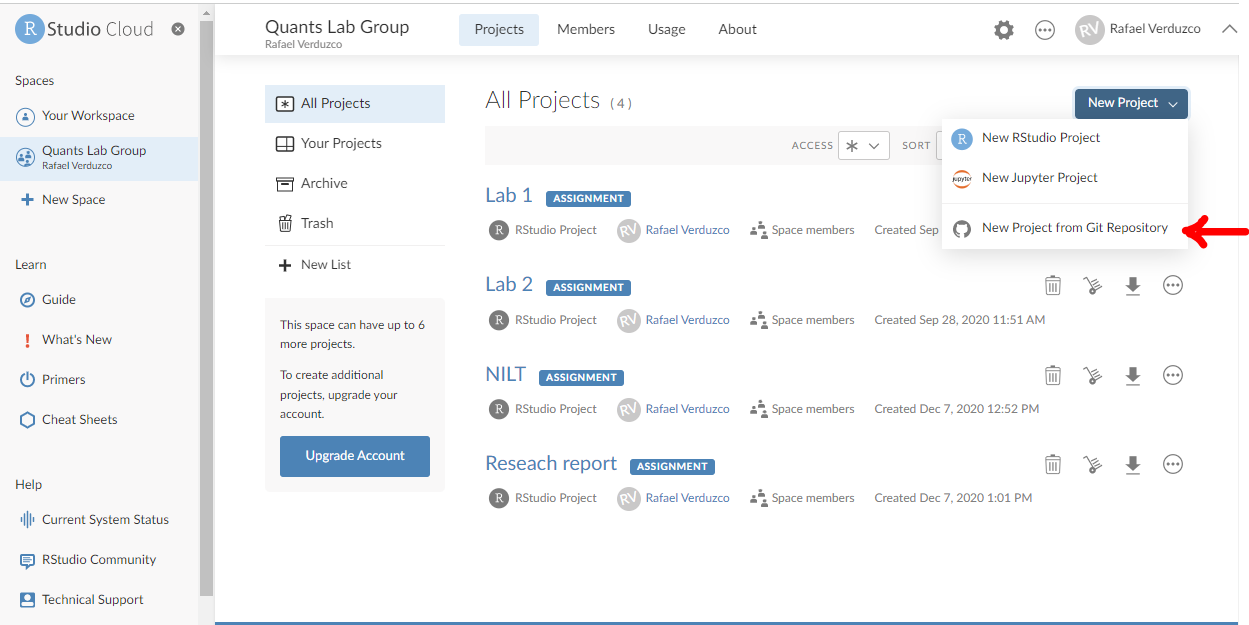
\includegraphics[width=1\linewidth]{./images/research_rep_2} \hfill{}

\caption{New project from GitHub.}

\label{fig:unnamed-chunk-114}
\textbackslash end\{figure\}
4. Paste the following URL in the box and click `OK': \url{https://github.com/rafavdz/UGQuant-assignment2}.
5. You are all set! Just click on the project to access the contents.

\hypertarget{rstudio-desktop-version}{%
\subsection{RStudio Desktop version}\label{rstudio-desktop-version}}

If alternately you decide to write your assessment using the RStudio Desktop version, consider the following steps:

\begin{enumerate}
\def\labelenumi{\arabic{enumi}.}
\tightlist
\item
  Access the following GitHub repository copying and pasting the following URL in your browser: \url{https://github.com/rafavdz/UGQuant-assignment2}.
\item
  Click on the `Code' button and select the `Download ZIP' option, as shown below.
  \textbackslash begin\{figure\}
\end{enumerate}

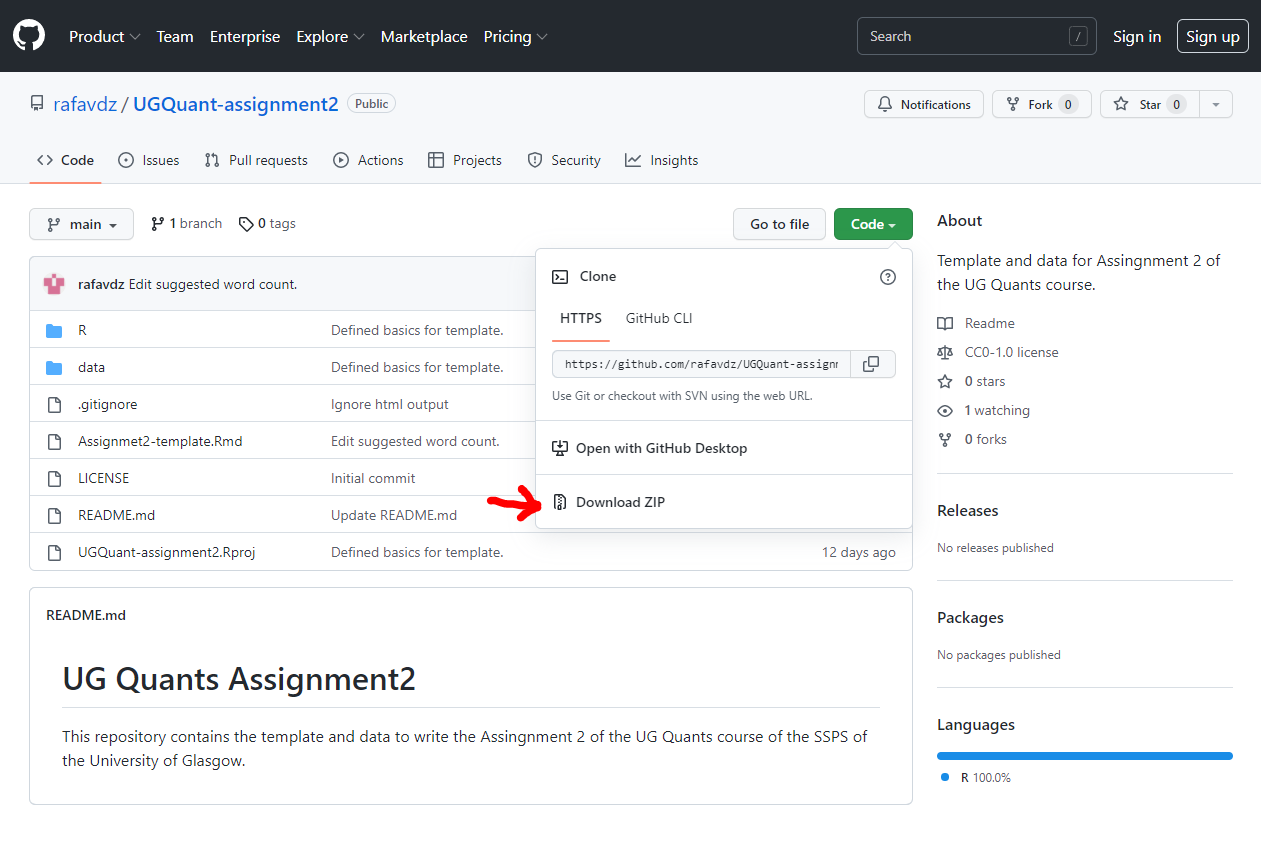
\includegraphics[width=1\linewidth]{./images/research_rep_4} \hfill{}

\caption{Downlowad ZIP from GitHub.}

\label{fig:unnamed-chunk-115}
\textbackslash end\{figure\}
3. Go to your local downloads folder, right click on the \texttt{UGQuant-assignment2-main.zip} and choose the `Extract all' option (here, you can also chose the folder where you want to store the RStudio project and write your assignment).
4. Click on the `Extract' button.
5. As you can see, this folder contains an RStudio project. Open the \texttt{UGQuant-assignment2.Rproj} which will initialize a new RStudio session.

\hypertarget{about-the-research-report-template}{%
\section{About the research report template}\label{about-the-research-report-template}}

Once in your \textbf{UGQuant-assignment2} project, open the \texttt{Assignmet2-template.Rmd} file in Pane 4 under the `Files' tab, as shown below.

\begin{figure}

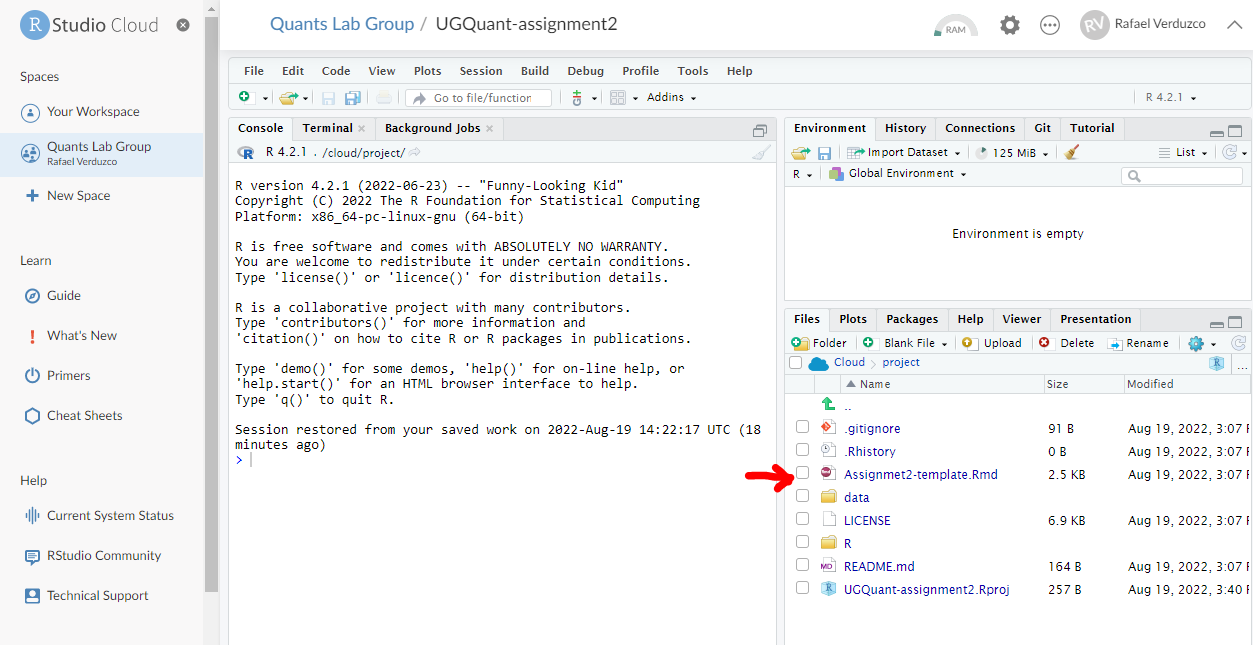
\includegraphics[width=1\linewidth]{./images/research_rep_3} \hfill{}

\caption{Template.}\label{fig:unnamed-chunk-116}
\end{figure}

This template contains the following:

\begin{itemize}
\tightlist
\item
  Suggested structure of the report.
\item
  Suggested word count for each section.
\item
  The code necessary to run and present the results of a multivariate linear regression.
\end{itemize}

In essence, this is the basic structure to start writing your assignment. Of course, you can add, edit, and customize as much as you consider appropriate. Remember, this is just a generic suggestion and you should still address all the points to the best of your abilities. \textbf{Remember: There are no hard and fast rules to say what's right or wrong.} You are the one who can determine and justify why you did what you did. There are also many ways to write and approach this assignment, so make choices based on your own interest(s) and disciplinary background. It is truly your time to shine! The course handbook also gives important pointers on how your report will be assessed, offering some guiding questions to tackle the report--don't skip this crucial step.

\hypertarget{activity-1-3}{%
\section{Activity 1}\label{activity-1-3}}

\begin{enumerate}
\def\labelenumi{\arabic{enumi}.}
\tightlist
\item
  In the template, fill in the `author' and `date' space in the YAML at the top of the file with your student number and appropriate information using quotation marks.
\item
  Knit the \texttt{Rmd} file as \texttt{html} (RStudio will ask to install some packages, click `Yes').
\item
  In the output, look at the results of the table under the `Results' section and identify the \emph{dependent} and the \emph{independent} variables. You can learn about the meaning of these variables in the NILT documentation (\href{https://www.ark.ac.uk/teaching/NILT2012TeachingResources.pdf}{click here to access the documentation}).
\item
  Identify the variables that are significant in this model and the direction of the relationship.
\item
  Discuss your interpretations with your neighbour or tutor. You can refer back to \protect\hyperlink{simple-lm}{Lab 8} and \protect\hyperlink{multi-lm}{Lab 9} to refresh your memory.
\end{enumerate}

\hypertarget{activity-2-3}{%
\section{Activity 2}\label{activity-2-3}}

\begin{enumerate}
\def\labelenumi{\arabic{enumi}.}
\tightlist
\item
  Write one introductory paragraph in the `Introduction' section of the template according to the guidance provided and your preliminary insights.
\item
  Knit the document again.
\end{enumerate}

\hypertarget{conclusion}{%
\section{Conclusion}\label{conclusion}}

You are on the right track now!

We hope that by getting familiar with this setting, you will easily succeed in writing your research report using all the knowledge and skills acquired during this course. Take this session to ask questions about the assignment or the course in general as much as possible. This is the right time to have specialized one-to-one support from your tutors.

We wish you the best of luck! Get in touch with your tutors via email or, even better, post any questions you have about the assignment on your lab group discussion forum on Moodle, if you don't know where to start or get stuck. Don't suffer in silence. Remember your Tutors, lab group mates, and the teaching and admin team are here for you. Also don't forget coding is \emph{all} about \textbf{trial and error}, so it's completely normal to write / copy and paste some code, then get an error message, and basically for your code to not work. Keep chipping at it, which sometimes can take hours (if not days), until you can get it to work. That's a normal process even for professional data scientists and quantitative researchers! So do persevere and don't panic if you don't get it to work right away, because troubleshooting your code is part of the work, in addition to making your own choices in the analysis and reporting. For the code, the error message you get often gives you clues about, well, where the error is. So read the error message carefully, it might be you haven't loaded the package required to run the code (remember to do this every time you open RStudio) or you might have missed a parentheses, or you might have not capitalised a word in the R syntax when you need to. Double check the R cheatsheets or previous sections in the lab workbook to ensure you have specified R syntax/arguments correctly. Again, trial and error is your friend, unlike writing an essay/doing an exam.

Good luck and have fun! You got this.

\hypertarget{answers}{%
\chapter*{Workbook suggested answers}\label{answers}}
\addcontentsline{toc}{chapter}{Workbook suggested answers}

\hypertarget{introduction-4}{%
\section{Introduction}\label{introduction-4}}

This chapter presents the suggested \texttt{R} code to answer the workbook activities and exercises throughout the course labs in Quantitative Research Methods for Social Sciences. This covers from Lab 3 to Lab 9.

Before looking at the answers, try asking your tutor for help. Also, we strongly recommend web resources, such as \url{https://stackoverflow.com/} or \url{https://community.rstudio.com/}. By solving the issues, you will learn a lot! ;)

\hypertarget{lab-3.-data-wrangling}{%
\section{Lab 3. Data wrangling}\label{lab-3.-data-wrangling}}

\begin{Shaded}
\begin{Highlighting}[]
\DocumentationTok{\#\# Load the packages}
\FunctionTok{library}\NormalTok{(tidyverse)}

\CommentTok{\# Read the data from the .rds file}
\NormalTok{clean\_data }\OtherTok{\textless{}{-}} \FunctionTok{readRDS}\NormalTok{(}\StringTok{"data/nilt\_r\_object.rds"}\NormalTok{)}
\CommentTok{\# Glimpse clean\_data}
\FunctionTok{glimpse}\NormalTok{(clean\_data)}

\CommentTok{\# Glimpse the nilt data}
\FunctionTok{glimpse}\NormalTok{(nilt)}
\end{Highlighting}
\end{Shaded}

\hypertarget{lab-4.-exploratory-data-analysis}{%
\section{Lab 4. Exploratory data analysis}\label{lab-4.-exploratory-data-analysis}}

Preamble code

\begin{Shaded}
\begin{Highlighting}[]
\DocumentationTok{\#\# Load the packages}
\FunctionTok{library}\NormalTok{(tidyverse)}
\CommentTok{\# Read the data from the .rds file}
\NormalTok{nilt }\OtherTok{\textless{}{-}} \FunctionTok{readRDS}\NormalTok{(}\StringTok{"data/nilt\_r\_object.rds"}\NormalTok{)}
\end{Highlighting}
\end{Shaded}

\begin{Shaded}
\begin{Highlighting}[]
\CommentTok{\#Subset}
\NormalTok{nilt\_subset }\OtherTok{\textless{}{-}} \FunctionTok{select}\NormalTok{(nilt, rsex, rage, highqual, religcat, uninatid,  ruhappy, rhourswk, persinc2)}
\end{Highlighting}
\end{Shaded}

\hypertarget{activity-1-4}{%
\subsection{Activity \#1}\label{activity-1-4}}

From your R Studio Cloud script, do the following activities using the data stored in the \texttt{nilt\_subset} object:

\begin{itemize}
\tightlist
\item
  Create a One-Way contingency table for \texttt{uninatid} in the \texttt{nilt\_subset} dataset using the \texttt{sumtable()} function;
\end{itemize}

\begin{Shaded}
\begin{Highlighting}[]
\CommentTok{\# Load the vtable package to create summary tables}
\FunctionTok{library}\NormalTok{(vtable)}
\CommentTok{\# Create table}
\FunctionTok{sumtable}\NormalTok{(nilt\_subset, }\AttributeTok{vars =} \FunctionTok{c}\NormalTok{(}\StringTok{\textquotesingle{}uninatid\textquotesingle{}}\NormalTok{))}
\end{Highlighting}
\end{Shaded}

\begin{table}

\caption{\label{tab:unnamed-chunk-120}Summary Statistics}
\centering
\begin{tabular}[t]{lll}
\toprule
Variable & N & Percent\\
\midrule
uninatid & 1183 & \\
... Unionist & 348 & 29\%\\
... Nationalist & 255 & 22\%\\
... Neither & 580 & 49\%\\
\bottomrule
\end{tabular}
\end{table}

\begin{itemize}
\tightlist
\item
  Using the variables \texttt{religcat} and \texttt{uninatid}, generate a Two-Way contingency table;
\end{itemize}

\begin{Shaded}
\begin{Highlighting}[]
\FunctionTok{sumtable}\NormalTok{(nilt\_subset, }\AttributeTok{vars =} \FunctionTok{c}\NormalTok{(}\StringTok{\textquotesingle{}religcat\textquotesingle{}}\NormalTok{), }\AttributeTok{group =} \StringTok{\textquotesingle{}uninatid\textquotesingle{}}\NormalTok{)}
\end{Highlighting}
\end{Shaded}

\begin{table}

\caption{\label{tab:unnamed-chunk-121}Summary Statistics}
\centering
\begin{tabular}[t]{lllllll}
\toprule
\multicolumn{1}{c}{uninatid} & \multicolumn{2}{c}{Unionist} & \multicolumn{2}{c}{Nationalist} & \multicolumn{2}{c}{Neither} \\
\cmidrule(l{3pt}r{3pt}){1-1} \cmidrule(l{3pt}r{3pt}){2-3} \cmidrule(l{3pt}r{3pt}){4-5} \cmidrule(l{3pt}r{3pt}){6-7}
Variable & N & Percent & N & Percent & N & Percent\\
\midrule
religcat & 341 &  & 255 &  & 558 & \\
... Catholic & 2 & 1\% & 245 & 96\% & 238 & 43\%\\
... Protestant & 305 & 89\% & 5 & 2\% & 180 & 32\%\\
... No religion & 34 & 10\% & 5 & 2\% & 140 & 25\%\\
\bottomrule
\end{tabular}
\end{table}

\hypertarget{activity-2-4}{%
\subsection{Activity \#2}\label{activity-2-4}}

Using the data in the \texttt{nilt\_subset} object, complete the following activities.

\begin{itemize}
\tightlist
\item
  Using the \texttt{hist()} function plot a histogram of personal income \texttt{persinc2}. From the NILT documentation this variable refers to annual personal income in £ before taxes and other deductions;
\end{itemize}

\begin{Shaded}
\begin{Highlighting}[]
\FunctionTok{hist}\NormalTok{(nilt\_subset}\SpecialCharTok{$}\NormalTok{persinc2)}
\end{Highlighting}
\end{Shaded}

\begin{flushleft}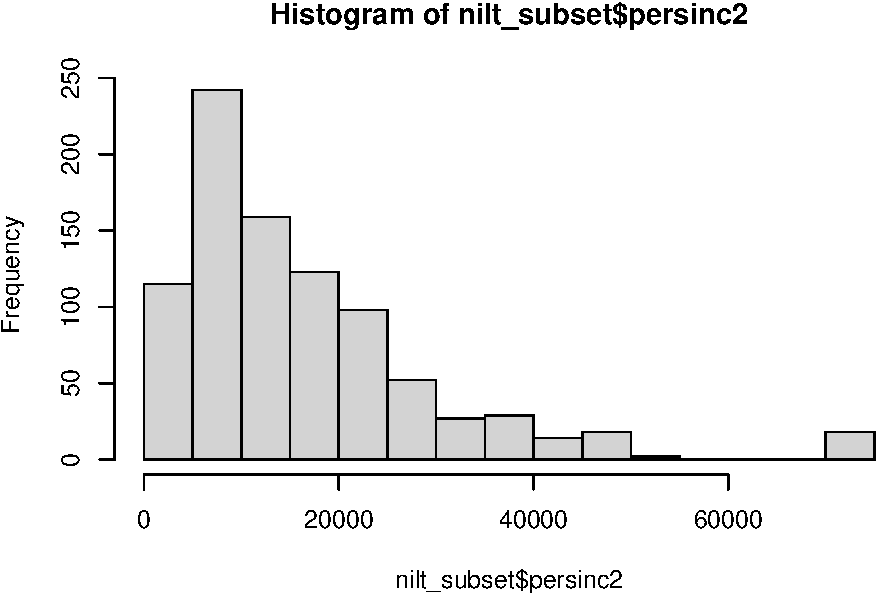
\includegraphics[width=1\linewidth]{lab-workbook_files/figure-latex/unnamed-chunk-122-1} \end{flushleft}

\begin{itemize}
\tightlist
\item
  Create a summary of the personal income \texttt{persinc2} variable, using the \texttt{sumtable()} function.
\end{itemize}

\begin{Shaded}
\begin{Highlighting}[]
\FunctionTok{sumtable}\NormalTok{(nilt\_subset, }\AttributeTok{vars =} \FunctionTok{c}\NormalTok{(}\StringTok{\textquotesingle{}persinc2\textquotesingle{}}\NormalTok{))}
\end{Highlighting}
\end{Shaded}

\begin{table}

\caption{\label{tab:unnamed-chunk-123}Summary Statistics}
\centering
\begin{tabular}[t]{llllllll}
\toprule
Variable & N & Mean & Std. Dev. & Min & Pctl. 25 & Pctl. 75 & Max\\
\midrule
persinc2 & 897 & 16395 & 13466 & 260 & 6760 & 22100 & 75000\\
\bottomrule
\end{tabular}
\end{table}

\begin{itemize}
\tightlist
\item
  Compute the mean and standard deviation of the personal income \texttt{persinc2}, grouped by happiness \texttt{ruhappy}.
\end{itemize}

\begin{Shaded}
\begin{Highlighting}[]
\FunctionTok{sumtable}\NormalTok{(nilt\_subset, }\AttributeTok{vars =} \FunctionTok{c}\NormalTok{(}\StringTok{\textquotesingle{}persinc2\textquotesingle{}}\NormalTok{), }\AttributeTok{group =} \StringTok{\textquotesingle{}ruhappy\textquotesingle{}}\NormalTok{)}
\end{Highlighting}
\end{Shaded}

\begin{table}

\caption{\label{tab:unnamed-chunk-124}Summary Statistics}
\centering
\begin{tabular}[t]{llllllllllllllll}
\toprule
\multicolumn{1}{c}{ruhappy} & \multicolumn{3}{c}{Very happy} & \multicolumn{3}{c}{Fairly happy} & \multicolumn{3}{c}{Not very happy} & \multicolumn{3}{c}{Not at all happy} & \multicolumn{3}{c}{Can't choose} \\
\cmidrule(l{3pt}r{3pt}){1-1} \cmidrule(l{3pt}r{3pt}){2-4} \cmidrule(l{3pt}r{3pt}){5-7} \cmidrule(l{3pt}r{3pt}){8-10} \cmidrule(l{3pt}r{3pt}){11-13} \cmidrule(l{3pt}r{3pt}){14-16}
Variable & N & Mean & SD & N & Mean & SD & N & Mean & SD & N & Mean & SD & N & Mean & SD\\
\midrule
persinc2 & 305 & 17569 & 13429 & 500 & 16262 & 14015 & 62 & 13445 & 9754 & 9 & 12451 & 11501 & 15 & 11457 & 6113\\
\bottomrule
\end{tabular}
\end{table}

\hypertarget{lab-6.-visual-exploratory-analysis}{%
\section{Lab 6. Visual exploratory analysis}\label{lab-6.-visual-exploratory-analysis}}

Preamble code

\begin{Shaded}
\begin{Highlighting}[]
\DocumentationTok{\#\# Load the packages}
\FunctionTok{library}\NormalTok{(tidyverse)}

\CommentTok{\# Load the data from the .rds file we created in the last lab}
\NormalTok{nilt }\OtherTok{\textless{}{-}} \FunctionTok{readRDS}\NormalTok{(}\StringTok{"data/nilt\_r\_object.rds"}\NormalTok{)}
\CommentTok{\#Create subset}
\NormalTok{nilt\_subset }\OtherTok{\textless{}{-}} \FunctionTok{select}\NormalTok{(nilt, rsex, rage, highqual, religcat, uninatid,  ruhappy, rhourswk, persinc2)}
\end{Highlighting}
\end{Shaded}

\hypertarget{excercices}{%
\subsection{Excercices}\label{excercices}}

Using the \texttt{nilt\_subset} object, complete the tasks below in the Rmd file `Lab\_4', which you created earlier. Insert a new chunk for each of these activities and include brief comments as text in the Rmd document to introduce the plots and discuss the results (tip ---leave an empty line between your text and the next chunk to separate the description and the plots):

\begin{itemize}
\tightlist
\item
  Create a first-level header to start a section called ``Categorical analysis'';
\end{itemize}

\begin{Shaded}
\begin{Highlighting}[]
\DocumentationTok{\#\# Categorical analysis}
\end{Highlighting}
\end{Shaded}

\begin{itemize}
\tightlist
\item
  Create a simple bar plot using the \texttt{geom\_bar()} geometry to visualize the political affiliation reported by the respondents using the variable \texttt{uninatid};
\end{itemize}

\begin{Shaded}
\begin{Highlighting}[]
\FunctionTok{ggplot}\NormalTok{(nilt\_subset, }\FunctionTok{aes}\NormalTok{(}\AttributeTok{x=}\NormalTok{uninatid)) }\SpecialCharTok{+}
  \FunctionTok{geom\_bar}\NormalTok{() }\SpecialCharTok{+}
  \FunctionTok{labs}\NormalTok{(}\AttributeTok{title =} \StringTok{"Political afiliation"}\NormalTok{, }\AttributeTok{x=} \StringTok{"Party"}\NormalTok{)}
\end{Highlighting}
\end{Shaded}

\begin{flushleft}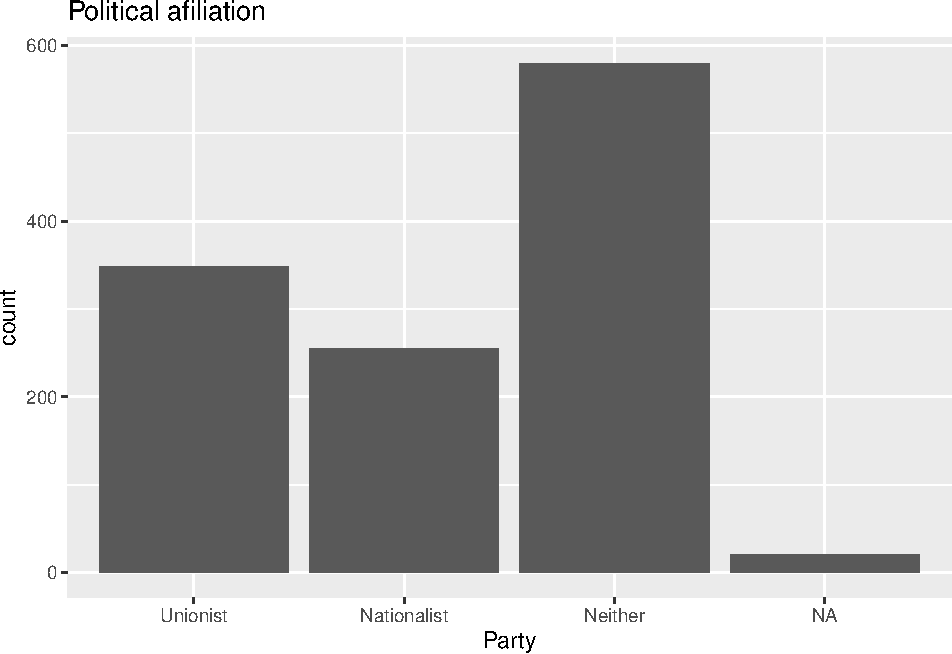
\includegraphics[width=1\linewidth]{lab-workbook_files/figure-latex/unnamed-chunk-127-1} \end{flushleft}

\begin{itemize}
\tightlist
\item
  Based on the plot above, create a `stacked bar plot' to visualize the political affiliation by religion, using the \texttt{uninatid} and \texttt{religcat} variables;
\end{itemize}

\begin{Shaded}
\begin{Highlighting}[]
\FunctionTok{ggplot}\NormalTok{(nilt\_subset, }\FunctionTok{aes}\NormalTok{(}\AttributeTok{x=}\NormalTok{uninatid, }\AttributeTok{fill =}\NormalTok{ religcat)) }\SpecialCharTok{+}
  \FunctionTok{geom\_bar}\NormalTok{() }\SpecialCharTok{+}
  \FunctionTok{labs}\NormalTok{(}\AttributeTok{title =} \StringTok{"Political afiliation by religion"}\NormalTok{, }
       \AttributeTok{x=} \StringTok{"Party"}\NormalTok{, }\AttributeTok{fill =} \StringTok{"Religion"}\NormalTok{)}
\end{Highlighting}
\end{Shaded}

\begin{flushleft}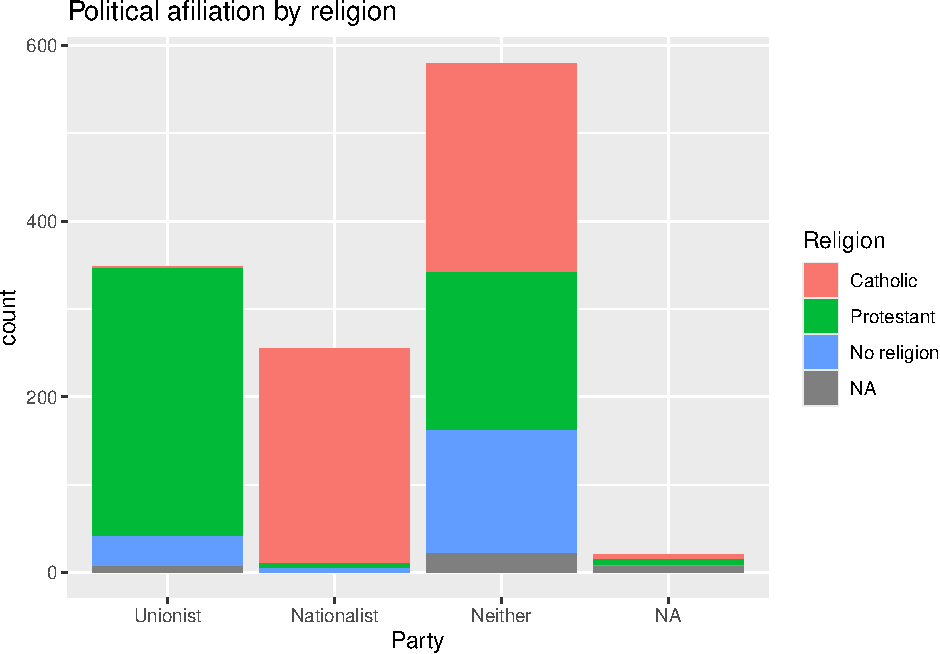
\includegraphics[width=1\linewidth]{lab-workbook_files/figure-latex/unnamed-chunk-128-1} \end{flushleft}

\begin{itemize}
\tightlist
\item
  Create a new first-level header to start a section called ``Numeric analysis'';
\end{itemize}

\begin{Shaded}
\begin{Highlighting}[]
\DocumentationTok{\#\# Numeric analysis}
\end{Highlighting}
\end{Shaded}

\begin{itemize}
\tightlist
\item
  Create a scatter plot about the relationship between personal income \texttt{persinc2} on the Y axis and number of hours worked a week \texttt{rhourswk} on the X axis;
\end{itemize}

\begin{Shaded}
\begin{Highlighting}[]
\FunctionTok{ggplot}\NormalTok{(nilt\_subset, }\FunctionTok{aes}\NormalTok{(}\AttributeTok{x=}\NormalTok{ rhourswk, }\AttributeTok{y=}\NormalTok{persinc2)) }\SpecialCharTok{+}
  \FunctionTok{geom\_point}\NormalTok{() }\SpecialCharTok{+}
  \FunctionTok{labs}\NormalTok{(}\AttributeTok{title=} \StringTok{\textquotesingle{}Income and number of hours worked a week\textquotesingle{}}\NormalTok{,}
       \AttributeTok{x =} \StringTok{\textquotesingle{}Number of hours worked a week\textquotesingle{}}\NormalTok{, }\AttributeTok{y=} \StringTok{\textquotesingle{}Personal income (£ a year)\textquotesingle{}}\NormalTok{ )}
\end{Highlighting}
\end{Shaded}

\begin{flushleft}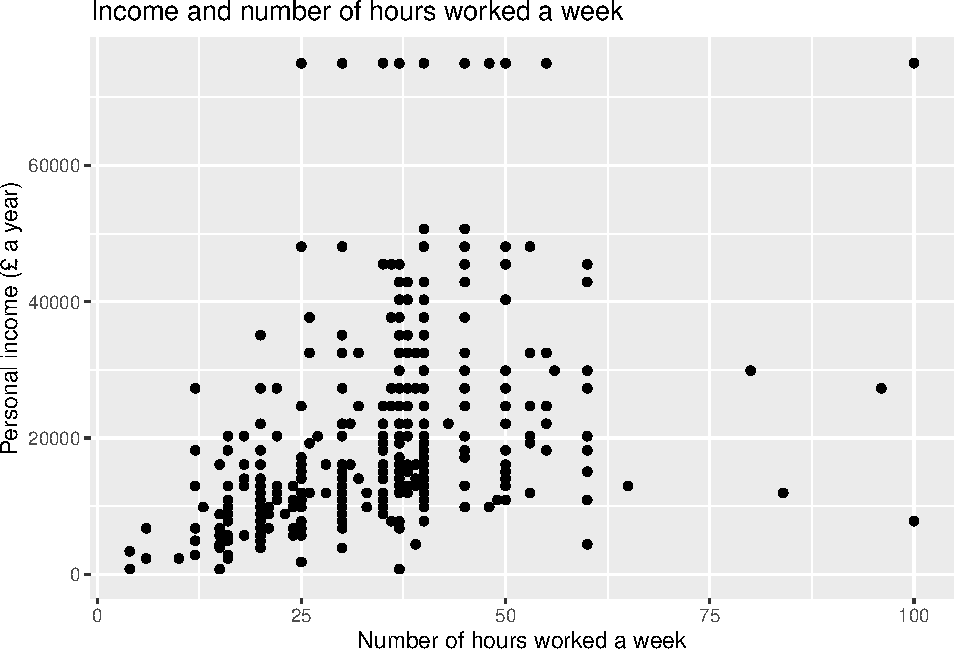
\includegraphics[width=1\linewidth]{lab-workbook_files/figure-latex/unnamed-chunk-130-1} \end{flushleft}

\begin{itemize}
\tightlist
\item
  Finally, create a box plot to visualize personal income \texttt{persinc2} on the Y axis and self-reported level of happiness \texttt{ruhappy} on the x axis\ldots{} Interesting result, Isn't it? Talk to your lab group-mates and tutors about your results on Zoom (live) or your Lab Group on Teams (online anytime);
\end{itemize}

\begin{Shaded}
\begin{Highlighting}[]
\FunctionTok{ggplot}\NormalTok{(nilt\_subset, }\FunctionTok{aes}\NormalTok{(}\AttributeTok{x=}\NormalTok{ ruhappy, }\AttributeTok{y=}\NormalTok{persinc2)) }\SpecialCharTok{+}
  \FunctionTok{geom\_boxplot}\NormalTok{() }\SpecialCharTok{+}
  \FunctionTok{labs}\NormalTok{(}\AttributeTok{title=} \StringTok{\textquotesingle{}Personal income and happiness\textquotesingle{}}\NormalTok{, }
       \AttributeTok{x=}\StringTok{\textquotesingle{}Hapiness level\textquotesingle{}}\NormalTok{, }\AttributeTok{y=}\StringTok{\textquotesingle{}Personal income (£ a year)\textquotesingle{}}\NormalTok{)}
\end{Highlighting}
\end{Shaded}

\begin{flushleft}\includegraphics[width=1\linewidth]{lab-workbook_files/figure-latex/unnamed-chunk-131-1} \end{flushleft}

\begin{itemize}
\tightlist
\item
  Briefly comment each of the plots as text in your Rmd file;
\item
  Knit the .Rmd document as HTML or PDF. The knitted file will be saved automatically in your project. You can come back to the Rmd file to make changes if needed and knit it again as many times as you wish.
\end{itemize}

\hypertarget{lab-7.-correlation}{%
\section{Lab 7. Correlation}\label{lab-7.-correlation}}

\begin{Shaded}
\begin{Highlighting}[]
\DocumentationTok{\#\# Load the packages}
\FunctionTok{library}\NormalTok{(tidyverse)}
\CommentTok{\# Load the data from the .rds file we created in lab 3}
\NormalTok{nilt }\OtherTok{\textless{}{-}} \FunctionTok{readRDS}\NormalTok{(}\StringTok{"data/nilt\_r\_object.rds"}\NormalTok{)}
\end{Highlighting}
\end{Shaded}

\begin{Shaded}
\begin{Highlighting}[]
\CommentTok{\# Age of respondent’s spouse/partner}
\NormalTok{nilt}\SpecialCharTok{$}\NormalTok{spage }\OtherTok{\textless{}{-}} \FunctionTok{as.numeric}\NormalTok{(nilt}\SpecialCharTok{$}\NormalTok{spage)}
\CommentTok{\# Migration}
\NormalTok{nilt }\OtherTok{\textless{}{-}} \FunctionTok{mutate\_at}\NormalTok{(nilt, }\FunctionTok{vars}\NormalTok{(mil10yrs, miecono, micultur), as.numeric)}
\end{Highlighting}
\end{Shaded}

\begin{Shaded}
\begin{Highlighting}[]
\CommentTok{\# overall perception towards migrants}
\NormalTok{nilt }\OtherTok{\textless{}{-}} \FunctionTok{rowwise}\NormalTok{(nilt) }\SpecialCharTok{\%\textgreater{}\%} 
  \CommentTok{\# sum values}
  \FunctionTok{mutate}\NormalTok{(}\AttributeTok{mig\_per =} \FunctionTok{sum}\NormalTok{(mil10yrs, miecono, micultur, }\AttributeTok{na.rm =}\NormalTok{ T )) }\SpecialCharTok{\%\textgreater{}\%} 
  \FunctionTok{ungroup}\NormalTok{() }\SpecialCharTok{\%\textgreater{}\%} 
  \CommentTok{\# assign NA to values that sum 0}
  \FunctionTok{mutate}\NormalTok{(}\AttributeTok{mig\_per =}  \FunctionTok{na\_if}\NormalTok{(mig\_per, }\DecValTok{0}\NormalTok{))}
\end{Highlighting}
\end{Shaded}

\hypertarget{activity-1-5}{%
\subsection{Activity 1}\label{activity-1-5}}

Using the \texttt{nilt} data object, visualize the relationship of the following variables by creating a new chunk. Run the chunk individually and comment on what you observe from the result as text in the Rmd file (remember to leave an empty line between your text and the chunk).

\begin{itemize}
\tightlist
\item
  Create a scatter plot to visualize the correlation between the respondent's overall opinion in relation to migration \texttt{mig\_per} and the respondent's age \texttt{rage}. Remember that we just created the \texttt{mig\_per} variable by summing three variables which were in a 0-10 scale (the higher the value, the better the person's perception is). In \texttt{aes()}, specify \texttt{rage} on the X axis and \texttt{mig\_per} on the Y axis. Use the \texttt{ggplot()} function and \texttt{geom\_point()}. Also, include a straight line describing the points using the \texttt{geom\_smooth()} function. Within this function, set the \texttt{method} argument to \texttt{\textquotesingle{}lm\textquotesingle{}}.
\end{itemize}

\begin{Shaded}
\begin{Highlighting}[]
\FunctionTok{ggplot}\NormalTok{(nilt, }\FunctionTok{aes}\NormalTok{(}\AttributeTok{x=}\NormalTok{rage, mig\_per)) }\SpecialCharTok{+}
  \FunctionTok{geom\_point}\NormalTok{() }\SpecialCharTok{+}
  \FunctionTok{geom\_smooth}\NormalTok{(}\AttributeTok{method =} \StringTok{\textquotesingle{}lm\textquotesingle{}}\NormalTok{) }\SpecialCharTok{+}
  \FunctionTok{labs}\NormalTok{(}\AttributeTok{title =} \StringTok{\textquotesingle{}Perception of migration vs age\textquotesingle{}}\NormalTok{,}
       \AttributeTok{x=} \StringTok{\textquotesingle{}Respondent age\textquotesingle{}}\NormalTok{, }\AttributeTok{y=} \StringTok{\textquotesingle{}Perception of migration (0{-}30)\textquotesingle{}}\NormalTok{)}
\end{Highlighting}
\end{Shaded}

\begin{flushleft}\includegraphics[width=1\linewidth]{lab-workbook_files/figure-latex/unnamed-chunk-135-1} \end{flushleft}

\begin{itemize}
\tightlist
\item
  What type of relationship do you observe? Comment the overall result of the plot and whether this is in line with your previous expectation.
\end{itemize}

\hypertarget{lab-8.-linear-model.-simple-linear-regression}{%
\section{Lab 8. Linear model. Simple linear regression}\label{lab-8.-linear-model.-simple-linear-regression}}

\begin{Shaded}
\begin{Highlighting}[]
\DocumentationTok{\#\# Load the packages}
\FunctionTok{library}\NormalTok{(tidyverse)}
\CommentTok{\# Read the data from the .rds file}
\NormalTok{nilt }\OtherTok{\textless{}{-}} \FunctionTok{readRDS}\NormalTok{(}\StringTok{"data/nilt\_r\_object.rds"}\NormalTok{)}
\end{Highlighting}
\end{Shaded}

\begin{Shaded}
\begin{Highlighting}[]
\NormalTok{m3 }\OtherTok{\textless{}{-}} \FunctionTok{lm}\NormalTok{(persinc2 }\SpecialCharTok{\textasciitilde{}}\NormalTok{ rhourswk, }\AttributeTok{data =}\NormalTok{ nilt)}
\end{Highlighting}
\end{Shaded}

\hypertarget{lab-activities-2}{%
\subsection{Lab activities}\label{lab-activities-2}}

Use the \texttt{nilt} data set object in your \texttt{linear\_model\_intro} file to:

\begin{enumerate}
\def\labelenumi{\arabic{enumi}.}
\tightlist
\item
  Plot a scatter plot using \texttt{ggplot}. In the aesthetics, locate \texttt{rhourswk} in the X axis, and \texttt{persinc2} in the Y axis. In the \texttt{geom\_point()}, jitter the points by specifying the \texttt{position\ =\ \textquotesingle{}jitter\textquotesingle{}}. Also, include the best fit line using the \texttt{geom\_smooth()} function, and specify the \texttt{method\ =\ \textquotesingle{}lm\textquotesingle{}} inside.
\end{enumerate}

\begin{Shaded}
\begin{Highlighting}[]
\FunctionTok{ggplot}\NormalTok{(nilt, }\FunctionTok{aes}\NormalTok{(}\AttributeTok{x=}\NormalTok{ rhourswk, }\AttributeTok{y=}\NormalTok{ persinc2)) }\SpecialCharTok{+}
  \FunctionTok{geom\_point}\NormalTok{(}\AttributeTok{position =} \StringTok{\textquotesingle{}jitter\textquotesingle{}}\NormalTok{) }\SpecialCharTok{+}
  \FunctionTok{geom\_smooth}\NormalTok{(}\AttributeTok{method =} \StringTok{\textquotesingle{}lm\textquotesingle{}}\NormalTok{)}
\end{Highlighting}
\end{Shaded}

\begin{flushleft}\includegraphics[width=1\linewidth]{lab-workbook_files/figure-latex/unnamed-chunk-138-1} \end{flushleft}

\begin{enumerate}
\def\labelenumi{\arabic{enumi}.}
\setcounter{enumi}{1}
\tightlist
\item
  Print the summary of \texttt{m3} using the \texttt{summary()} function.
\end{enumerate}

\begin{Shaded}
\begin{Highlighting}[]
\FunctionTok{summary}\NormalTok{(m3)}
\end{Highlighting}
\end{Shaded}

\begin{verbatim}
## 
## Call:
## lm(formula = persinc2 ~ rhourswk, data = nilt)
## 
## Residuals:
##    Min     1Q Median     3Q    Max 
## -43694  -8148  -3070   4990  58249 
## 
## Coefficients:
##             Estimate Std. Error t value Pr(>|t|)    
## (Intercept)   5170.4     1966.2    2.63  0.00884 ** 
## rhourswk       463.2       52.4    8.84  < 2e-16 ***
## ---
## Signif. codes:  0 '***' 0.001 '**' 0.01 '*' 0.05 '.' 0.1 ' ' 1
## 
## Residual standard error: 13860 on 455 degrees of freedom
##   (747 observations deleted due to missingness)
## Multiple R-squared:  0.1466, Adjusted R-squared:  0.1447 
## F-statistic: 78.15 on 1 and 455 DF,  p-value: < 2.2e-16
\end{verbatim}

\begin{enumerate}
\def\labelenumi{\arabic{enumi}.}
\setcounter{enumi}{2}
\tightlist
\item
  Is the the relationship of hours worked a week significant?
  Re: Yes. The p-value (fourth column of the `Coefficients' table) is lower than 0.05.
\item
  What is the adjusted r-squared? How would you interpret it?
  Re: the adjusted R-squared is 0.14. This can be interpreted in terms of percentage, e.g.~14\% of the variance in personal income can be explained by the number of hours worked a week.
\item
  What is the sample size to fit the model?
  Re: The total number of observations in the data set is 1,204 and the model summary says that 747 observations were deleted due to missingness. Therefore, the sample size is 457 (1204-747).
\item
  What is the expected income in pounds a year for a respondent who works 30 hours a week according to coefficients of this model?
\end{enumerate}

\begin{Shaded}
\begin{Highlighting}[]
\FloatTok{5170.4} \SpecialCharTok{+} \FloatTok{463.2} \SpecialCharTok{*} \DecValTok{30}
\end{Highlighting}
\end{Shaded}

\begin{verbatim}
## [1] 19066.4
\end{verbatim}

\begin{enumerate}
\def\labelenumi{\arabic{enumi}.}
\setcounter{enumi}{6}
\tightlist
\item
  Plot a histogram of the residuals of \texttt{m3} using the \texttt{residuals()} function inside \texttt{hist()}. Do the residuals look normally distributed (as in a bell-shaped curve)?
\end{enumerate}

\begin{Shaded}
\begin{Highlighting}[]
\FunctionTok{hist}\NormalTok{(}\FunctionTok{residuals}\NormalTok{(m3))}
\end{Highlighting}
\end{Shaded}

\begin{flushleft}\includegraphics[width=1\linewidth]{lab-workbook_files/figure-latex/unnamed-chunk-141-1} \end{flushleft}

Overall, the residuals look normally distributed with the exception of the values to the right-hand side of the plot (between 40000 and 60000).

\hypertarget{lab-9.-multivariate-linear-model}{%
\section{Lab 9. Multivariate linear model}\label{lab-9.-multivariate-linear-model}}

\hypertarget{lab-activities-3}{%
\subsection{Lab activities}\label{lab-activities-3}}

\begin{enumerate}
\def\labelenumi{\arabic{enumi}.}
\tightlist
\item
  Load the packages, and the data that you will need in your file using the code below:
\end{enumerate}

\begin{Shaded}
\begin{Highlighting}[]
\DocumentationTok{\#\# Load the packages}
\FunctionTok{library}\NormalTok{(moderndive)}
\FunctionTok{library}\NormalTok{(tidyverse)}
\CommentTok{\# Read the data from the .rds file}
\NormalTok{nilt }\OtherTok{\textless{}{-}} \FunctionTok{readRDS}\NormalTok{(}\StringTok{"data/nilt\_r\_object.rds"}\NormalTok{)}
\end{Highlighting}
\end{Shaded}

\begin{enumerate}
\def\labelenumi{\arabic{enumi}.}
\setcounter{enumi}{1}
\tightlist
\item
  Print a table for the highest level of qualification \texttt{highqual} using the \texttt{table()} function.
\end{enumerate}

\begin{Shaded}
\begin{Highlighting}[]
\FunctionTok{table}\NormalTok{(nilt}\SpecialCharTok{$}\NormalTok{highqual)}
\end{Highlighting}
\end{Shaded}

\begin{verbatim}
## 
## Degree level or higher       Higher education   GCE A level or equiv 
##                    230                    102                    243 
##      GCSE A-C or equiv      GCSE D-G or equiv      No qualifications 
##                    185                     82                    281 
##   Other, level unknown           Unclassified 
##                     27                     54
\end{verbatim}

\begin{enumerate}
\def\labelenumi{\arabic{enumi}.}
\setcounter{enumi}{2}
\tightlist
\item
  Generate a scatter plot using \texttt{ggplot}. Within \texttt{aes()}, locate the number of hours worked a week \texttt{rhourswk} on the X axis and the personal income \texttt{persinc2} on the Y axis, and specify the \texttt{color} of the dots by the highest level of qualification \texttt{highqual}. Use the \texttt{geom\_point()} function and `jitter' the points using the argument \texttt{position}. Add the parallel slopes using the \texttt{geom\_parallel\_slopes()} function and set the standard error \texttt{se} to \texttt{FALSE}. What is your interpretation of the plot? Write down your comments to introduce the plot.
\end{enumerate}

\begin{Shaded}
\begin{Highlighting}[]
\FunctionTok{ggplot}\NormalTok{(nilt, }\FunctionTok{aes}\NormalTok{(}\AttributeTok{x =}\NormalTok{ rhourswk, }\AttributeTok{y=}\NormalTok{ persinc2, }\AttributeTok{color =}\NormalTok{ highqual)) }\SpecialCharTok{+}
  \FunctionTok{geom\_point}\NormalTok{(}\AttributeTok{position =} \StringTok{\textquotesingle{}jitter\textquotesingle{}}\NormalTok{) }\SpecialCharTok{+}
\NormalTok{  moderndive}\SpecialCharTok{::}\FunctionTok{geom\_parallel\_slopes}\NormalTok{(}\AttributeTok{se =} \ConstantTok{FALSE}\NormalTok{) }\SpecialCharTok{+}
  \FunctionTok{labs}\NormalTok{(}\AttributeTok{title =} \StringTok{"Personal income"}\NormalTok{,}
       \AttributeTok{subtitle =} \StringTok{\textquotesingle{}Personal income and number of hours worked a week by education level\textquotesingle{}}\NormalTok{,}
       \AttributeTok{x=} \StringTok{\textquotesingle{}Number of hours worked a week\textquotesingle{}}\NormalTok{, }\AttributeTok{y=} \StringTok{\textquotesingle{}Personal income (£ a year)\textquotesingle{}}\NormalTok{, }
       \AttributeTok{color =} \StringTok{\textquotesingle{}Highest education level\textquotesingle{}}\NormalTok{)}
\end{Highlighting}
\end{Shaded}

\begin{flushleft}\includegraphics[width=1\linewidth]{lab-workbook_files/figure-latex/unnamed-chunk-144-1} \end{flushleft}

\begin{enumerate}
\def\labelenumi{\arabic{enumi}.}
\setcounter{enumi}{3}
\tightlist
\item
  Fit a linear model model using the \texttt{lm()} function to analyse the personal income \texttt{persinc2} using the number of works worked a week \texttt{rhourswk}, the highest level of qualification \texttt{highqual}, and the age of the respondent \texttt{rage} as independent variables. Store the model in an object called \texttt{m4} and print the summary.
\end{enumerate}

\begin{Shaded}
\begin{Highlighting}[]
\NormalTok{m4 }\OtherTok{\textless{}{-}} \FunctionTok{lm}\NormalTok{(persinc2 }\SpecialCharTok{\textasciitilde{}}\NormalTok{ rhourswk }\SpecialCharTok{+}\NormalTok{ rage }\SpecialCharTok{+}\NormalTok{ highqual, nilt)}
\FunctionTok{summary}\NormalTok{(m4)}
\end{Highlighting}
\end{Shaded}

\begin{verbatim}
## 
## Call:
## lm(formula = persinc2 ~ rhourswk + rage + highqual, data = nilt)
## 
## Residuals:
##    Min     1Q Median     3Q    Max 
## -36228  -6425  -1411   4635  54749 
## 
## Coefficients:
##                               Estimate Std. Error t value Pr(>|t|)    
## (Intercept)                    3904.64    2714.25   1.439    0.151    
## rhourswk                        444.79      45.32   9.814  < 2e-16 ***
## rage                            236.59      48.47   4.881 1.47e-06 ***
## highqualHigher education      -8164.91    1939.50  -4.210 3.09e-05 ***
## highqualGCE A level or equiv -12439.26    1563.42  -7.956 1.47e-14 ***
## highqualGCSE A-C or equiv    -13037.47    1703.07  -7.655 1.20e-13 ***
## highqualGCSE D-G or equiv    -11622.07    2665.38  -4.360 1.61e-05 ***
## highqualNo qualifications    -12968.10    2339.78  -5.542 5.11e-08 ***
## highqualOther, level unknown  15445.70    3334.75   4.632 4.76e-06 ***
## highqualUnclassified         -12399.58    2786.16  -4.450 1.08e-05 ***
## ---
## Signif. codes:  0 '***' 0.001 '**' 0.01 '*' 0.05 '.' 0.1 ' ' 1
## 
## Residual standard error: 11830 on 447 degrees of freedom
##   (747 observations deleted due to missingness)
## Multiple R-squared:  0.3887, Adjusted R-squared:  0.3764 
## F-statistic: 31.58 on 9 and 447 DF,  p-value: < 2.2e-16
\end{verbatim}

\begin{enumerate}
\def\labelenumi{\arabic{enumi}.}
\setcounter{enumi}{4}
\tightlist
\item
  Comment on the results of the model by mentioning which of the variables is significant and their respective p-value, the adjusted r-squared of the model, and the number of observations used to fit the model.
  Re: All the independent variables including the number of hours worked a week, age, and all the categories of highest qualification level compared to `Degree or higher' are significant to predict personal income in the model `m4', considering that the p-value is lower than 0.05. We can confirm this from the fourth column of the `Coefficients' table. The adjusted R-squared of the model is 0.37. This means that 37.6\% of the variance in personal income can be explained by these variables. The size of the sample used to fit this model is 457, considering that the `nilt' data set contains 1204 observations but 747 were deleted due to missingness (1204 - 747).
\item
  Plot a histogram of the residuals for model \texttt{m4}. Do they look normally distributed? Can we trust our estimates or would you advise to carry out further actions to verify the adequate interpretation of this model?
\end{enumerate}

\begin{Shaded}
\begin{Highlighting}[]
\FunctionTok{hist}\NormalTok{(}\FunctionTok{residuals}\NormalTok{(m4))}
\end{Highlighting}
\end{Shaded}

\begin{flushleft}\includegraphics[width=1\linewidth]{lab-workbook_files/figure-latex/unnamed-chunk-146-1} \end{flushleft}

The distribution of the residuals in `m4' look overall normally distributed. However, the distribution is not perfectly symmetric. Therefore, we would advice to conduct further checks to test the linear model assumptions.

  \bibliography{book.bib,packages.bib}

\end{document}
